% Options for packages loaded elsewhere
\PassOptionsToPackage{unicode}{hyperref}
\PassOptionsToPackage{hyphens}{url}
\PassOptionsToPackage{dvipsnames,svgnames,x11names}{xcolor}
%
\documentclass[
  letterpaper,
  DIV=11,
  numbers=noendperiod]{scrreprt}

\usepackage{amsmath,amssymb}
\usepackage{iftex}
\ifPDFTeX
  \usepackage[T1]{fontenc}
  \usepackage[utf8]{inputenc}
  \usepackage{textcomp} % provide euro and other symbols
\else % if luatex or xetex
  \usepackage{unicode-math}
  \defaultfontfeatures{Scale=MatchLowercase}
  \defaultfontfeatures[\rmfamily]{Ligatures=TeX,Scale=1}
\fi
\usepackage{lmodern}
\ifPDFTeX\else  
    % xetex/luatex font selection
\fi
% Use upquote if available, for straight quotes in verbatim environments
\IfFileExists{upquote.sty}{\usepackage{upquote}}{}
\IfFileExists{microtype.sty}{% use microtype if available
  \usepackage[]{microtype}
  \UseMicrotypeSet[protrusion]{basicmath} % disable protrusion for tt fonts
}{}
\makeatletter
\@ifundefined{KOMAClassName}{% if non-KOMA class
  \IfFileExists{parskip.sty}{%
    \usepackage{parskip}
  }{% else
    \setlength{\parindent}{0pt}
    \setlength{\parskip}{6pt plus 2pt minus 1pt}}
}{% if KOMA class
  \KOMAoptions{parskip=half}}
\makeatother
\usepackage{xcolor}
\usepackage{svg}
\setlength{\emergencystretch}{3em} % prevent overfull lines
\setcounter{secnumdepth}{5}
% Make \paragraph and \subparagraph free-standing
\ifx\paragraph\undefined\else
  \let\oldparagraph\paragraph
  \renewcommand{\paragraph}[1]{\oldparagraph{#1}\mbox{}}
\fi
\ifx\subparagraph\undefined\else
  \let\oldsubparagraph\subparagraph
  \renewcommand{\subparagraph}[1]{\oldsubparagraph{#1}\mbox{}}
\fi

\usepackage{color}
\usepackage{fancyvrb}
\newcommand{\VerbBar}{|}
\newcommand{\VERB}{\Verb[commandchars=\\\{\}]}
\DefineVerbatimEnvironment{Highlighting}{Verbatim}{commandchars=\\\{\}}
% Add ',fontsize=\small' for more characters per line
\usepackage{framed}
\definecolor{shadecolor}{RGB}{241,243,245}
\newenvironment{Shaded}{\begin{snugshade}}{\end{snugshade}}
\newcommand{\AlertTok}[1]{\textcolor[rgb]{0.68,0.00,0.00}{#1}}
\newcommand{\AnnotationTok}[1]{\textcolor[rgb]{0.37,0.37,0.37}{#1}}
\newcommand{\AttributeTok}[1]{\textcolor[rgb]{0.40,0.45,0.13}{#1}}
\newcommand{\BaseNTok}[1]{\textcolor[rgb]{0.68,0.00,0.00}{#1}}
\newcommand{\BuiltInTok}[1]{\textcolor[rgb]{0.00,0.23,0.31}{#1}}
\newcommand{\CharTok}[1]{\textcolor[rgb]{0.13,0.47,0.30}{#1}}
\newcommand{\CommentTok}[1]{\textcolor[rgb]{0.37,0.37,0.37}{#1}}
\newcommand{\CommentVarTok}[1]{\textcolor[rgb]{0.37,0.37,0.37}{\textit{#1}}}
\newcommand{\ConstantTok}[1]{\textcolor[rgb]{0.56,0.35,0.01}{#1}}
\newcommand{\ControlFlowTok}[1]{\textcolor[rgb]{0.00,0.23,0.31}{#1}}
\newcommand{\DataTypeTok}[1]{\textcolor[rgb]{0.68,0.00,0.00}{#1}}
\newcommand{\DecValTok}[1]{\textcolor[rgb]{0.68,0.00,0.00}{#1}}
\newcommand{\DocumentationTok}[1]{\textcolor[rgb]{0.37,0.37,0.37}{\textit{#1}}}
\newcommand{\ErrorTok}[1]{\textcolor[rgb]{0.68,0.00,0.00}{#1}}
\newcommand{\ExtensionTok}[1]{\textcolor[rgb]{0.00,0.23,0.31}{#1}}
\newcommand{\FloatTok}[1]{\textcolor[rgb]{0.68,0.00,0.00}{#1}}
\newcommand{\FunctionTok}[1]{\textcolor[rgb]{0.28,0.35,0.67}{#1}}
\newcommand{\ImportTok}[1]{\textcolor[rgb]{0.00,0.46,0.62}{#1}}
\newcommand{\InformationTok}[1]{\textcolor[rgb]{0.37,0.37,0.37}{#1}}
\newcommand{\KeywordTok}[1]{\textcolor[rgb]{0.00,0.23,0.31}{#1}}
\newcommand{\NormalTok}[1]{\textcolor[rgb]{0.00,0.23,0.31}{#1}}
\newcommand{\OperatorTok}[1]{\textcolor[rgb]{0.37,0.37,0.37}{#1}}
\newcommand{\OtherTok}[1]{\textcolor[rgb]{0.00,0.23,0.31}{#1}}
\newcommand{\PreprocessorTok}[1]{\textcolor[rgb]{0.68,0.00,0.00}{#1}}
\newcommand{\RegionMarkerTok}[1]{\textcolor[rgb]{0.00,0.23,0.31}{#1}}
\newcommand{\SpecialCharTok}[1]{\textcolor[rgb]{0.37,0.37,0.37}{#1}}
\newcommand{\SpecialStringTok}[1]{\textcolor[rgb]{0.13,0.47,0.30}{#1}}
\newcommand{\StringTok}[1]{\textcolor[rgb]{0.13,0.47,0.30}{#1}}
\newcommand{\VariableTok}[1]{\textcolor[rgb]{0.07,0.07,0.07}{#1}}
\newcommand{\VerbatimStringTok}[1]{\textcolor[rgb]{0.13,0.47,0.30}{#1}}
\newcommand{\WarningTok}[1]{\textcolor[rgb]{0.37,0.37,0.37}{\textit{#1}}}

\providecommand{\tightlist}{%
  \setlength{\itemsep}{0pt}\setlength{\parskip}{0pt}}\usepackage{longtable,booktabs,array}
\usepackage{calc} % for calculating minipage widths
% Correct order of tables after \paragraph or \subparagraph
\usepackage{etoolbox}
\makeatletter
\patchcmd\longtable{\par}{\if@noskipsec\mbox{}\fi\par}{}{}
\makeatother
% Allow footnotes in longtable head/foot
\IfFileExists{footnotehyper.sty}{\usepackage{footnotehyper}}{\usepackage{footnote}}
\makesavenoteenv{longtable}
\usepackage{graphicx}
\makeatletter
\def\maxwidth{\ifdim\Gin@nat@width>\linewidth\linewidth\else\Gin@nat@width\fi}
\def\maxheight{\ifdim\Gin@nat@height>\textheight\textheight\else\Gin@nat@height\fi}
\makeatother
% Scale images if necessary, so that they will not overflow the page
% margins by default, and it is still possible to overwrite the defaults
% using explicit options in \includegraphics[width, height, ...]{}
\setkeys{Gin}{width=\maxwidth,height=\maxheight,keepaspectratio}
% Set default figure placement to htbp
\makeatletter
\def\fps@figure{htbp}
\makeatother
% definitions for citeproc citations
\NewDocumentCommand\citeproctext{}{}
\NewDocumentCommand\citeproc{mm}{%
  \begingroup\def\citeproctext{#2}\cite{#1}\endgroup}
\makeatletter
 % allow citations to break across lines
 \let\@cite@ofmt\@firstofone
 % avoid brackets around text for \cite:
 \def\@biblabel#1{}
 \def\@cite#1#2{{#1\if@tempswa , #2\fi}}
\makeatother
\newlength{\cslhangindent}
\setlength{\cslhangindent}{1.5em}
\newlength{\csllabelwidth}
\setlength{\csllabelwidth}{3em}
\newenvironment{CSLReferences}[2] % #1 hanging-indent, #2 entry-spacing
 {\begin{list}{}{%
  \setlength{\itemindent}{0pt}
  \setlength{\leftmargin}{0pt}
  \setlength{\parsep}{0pt}
  % turn on hanging indent if param 1 is 1
  \ifodd #1
   \setlength{\leftmargin}{\cslhangindent}
   \setlength{\itemindent}{-1\cslhangindent}
  \fi
  % set entry spacing
  \setlength{\itemsep}{#2\baselineskip}}}
 {\end{list}}
\usepackage{calc}
\newcommand{\CSLBlock}[1]{\hfill\break\parbox[t]{\linewidth}{\strut\ignorespaces#1\strut}}
\newcommand{\CSLLeftMargin}[1]{\parbox[t]{\csllabelwidth}{\strut#1\strut}}
\newcommand{\CSLRightInline}[1]{\parbox[t]{\linewidth - \csllabelwidth}{\strut#1\strut}}
\newcommand{\CSLIndent}[1]{\hspace{\cslhangindent}#1}

\KOMAoption{captions}{tableheading}
\makeatletter
\@ifpackageloaded{tcolorbox}{}{\usepackage[skins,breakable]{tcolorbox}}
\@ifpackageloaded{fontawesome5}{}{\usepackage{fontawesome5}}
\definecolor{quarto-callout-color}{HTML}{909090}
\definecolor{quarto-callout-note-color}{HTML}{0758E5}
\definecolor{quarto-callout-important-color}{HTML}{CC1914}
\definecolor{quarto-callout-warning-color}{HTML}{EB9113}
\definecolor{quarto-callout-tip-color}{HTML}{00A047}
\definecolor{quarto-callout-caution-color}{HTML}{FC5300}
\definecolor{quarto-callout-color-frame}{HTML}{acacac}
\definecolor{quarto-callout-note-color-frame}{HTML}{4582ec}
\definecolor{quarto-callout-important-color-frame}{HTML}{d9534f}
\definecolor{quarto-callout-warning-color-frame}{HTML}{f0ad4e}
\definecolor{quarto-callout-tip-color-frame}{HTML}{02b875}
\definecolor{quarto-callout-caution-color-frame}{HTML}{fd7e14}
\makeatother
\makeatletter
\@ifpackageloaded{bookmark}{}{\usepackage{bookmark}}
\makeatother
\makeatletter
\@ifpackageloaded{caption}{}{\usepackage{caption}}
\AtBeginDocument{%
\ifdefined\contentsname
  \renewcommand*\contentsname{Table of contents}
\else
  \newcommand\contentsname{Table of contents}
\fi
\ifdefined\listfigurename
  \renewcommand*\listfigurename{List of Figures}
\else
  \newcommand\listfigurename{List of Figures}
\fi
\ifdefined\listtablename
  \renewcommand*\listtablename{List of Tables}
\else
  \newcommand\listtablename{List of Tables}
\fi
\ifdefined\figurename
  \renewcommand*\figurename{Figure}
\else
  \newcommand\figurename{Figure}
\fi
\ifdefined\tablename
  \renewcommand*\tablename{Table}
\else
  \newcommand\tablename{Table}
\fi
}
\@ifpackageloaded{float}{}{\usepackage{float}}
\floatstyle{ruled}
\@ifundefined{c@chapter}{\newfloat{codelisting}{h}{lop}}{\newfloat{codelisting}{h}{lop}[chapter]}
\floatname{codelisting}{Listing}
\newcommand*\listoflistings{\listof{codelisting}{List of Listings}}
\makeatother
\makeatletter
\makeatother
\makeatletter
\@ifpackageloaded{caption}{}{\usepackage{caption}}
\@ifpackageloaded{subcaption}{}{\usepackage{subcaption}}
\makeatother
\ifLuaTeX
  \usepackage{selnolig}  % disable illegal ligatures
\fi
\usepackage{bookmark}

\IfFileExists{xurl.sty}{\usepackage{xurl}}{} % add URL line breaks if available
\urlstyle{same} % disable monospaced font for URLs
\hypersetup{
  pdftitle={AstroParticles},
  pdfauthor={J. A. Aguilar},
  colorlinks=true,
  linkcolor={blue},
  filecolor={Maroon},
  citecolor={Blue},
  urlcolor={Blue},
  pdfcreator={LaTeX via pandoc}}

\title{AstroParticles}
\author{J. A. Aguilar}
\date{2024-01-31}

\begin{document}
\maketitle

\renewcommand*\contentsname{Table of contents}
{
\hypersetup{linkcolor=}
\setcounter{tocdepth}{2}
\tableofcontents
}
\bookmarksetup{startatroot}

\chapter*{Preface}\label{preface}
\addcontentsline{toc}{chapter}{Preface}

\markboth{Preface}{Preface}

This is a book on astroparticle physics created from markdown and
executable code in \texttt{python}.

\section*{Why Python?}\label{why-python}
\addcontentsline{toc}{section}{Why Python?}

\markright{Why Python?}

Although certainly is not a requirement to understand the physics
processes involved in astroparticle phenomena, it is beneficial to
resolve numerically some of the proposed problems in order to better
assimilate the concepts discussed during this course. The python
programming language is used as a tool for constructing these numerical
solutions. The advantage is that there exist complete mathematical
libraries (\texttt{numpy/scipy}) for python, astronomical and analysis
toolboxes (\texttt{astropy/healpy}), as well as powerful graphical
visualization frameworks (matplotlib), which make it possible to easily
construct problem solvers in a matter of minutes along with its
graphical output. The idea is also to familiarize with what has become
one of the most popular analysis tools in the high-energy physics as
well as in the astronomy communities. A long this week we will use the
following python modules related with astroparticle physics:

\begin{itemize}
\tightlist
\item
  \texttt{astropy}
\item
  \texttt{healpy}
\item
  \texttt{gammapy}
\item
  \texttt{crdb}
\end{itemize}

\textbf{References will be added}

\subsection*{Disclaimer and
Acknowledgments}\label{disclaimer-and-acknowledgments}
\addcontentsline{toc}{subsection}{Disclaimer and Acknowledgments}

These notes are far from original work. I limited myself to read the
literature on the subject, assimilate and also re-elaborate concepts
into what I hope is a coherent story, useful to give a feeling of how
wonderful our universe and Nature are. There is an endless list of
people that inspired these notes and many references. Particularly, we
acknowledge: T.K. Gaisser, F. Halzen, K. Hanson, Alexander Kappes,
Carlos de los Heros, Stefano Gabici, T. Montaruli, and a long etc.

\bookmarksetup{startatroot}

\chapter*{Basic Concents and
Notations}\label{basic-concents-and-notations}
\addcontentsline{toc}{chapter}{Basic Concents and Notations}

\markboth{Basic Concents and Notations}{Basic Concents and Notations}

\section*{The Computational
Framework}\label{the-computational-framework}
\addcontentsline{toc}{section}{The Computational Framework}

\markright{The Computational Framework}

In this part we are going to review the concepts that we will use in the
rest of the course. It will also serve to set up the conventions, units,
etc.

\subsection*{Natural Units}\label{natural-units}
\addcontentsline{toc}{subsection}{Natural Units}

In high energy physics and astro-particle physics it is very common to
use the natural units where \(\hbar = c = 1\). The correspondence
between natural units and physical units can be established by use of

\[\hbar = 6.58 \times 10^{-16} {\;\mathrm{ GeV}\cdot \mathrm{ ns}} = 1\;\Rightarrow 1\;\mathrm{ GeV} = 1.52 \times 10^{15}\;{\mathrm{ ns}^{-1}}\]

\[c = 30.0\;\mathrm{ cm/ns} = 1 \Rightarrow 30\;\mathrm{ cm} = 1\;\mathrm{ ns}\]

In these units there is then only one fundamental dimension:

\begin{itemize}
\tightlist
\item
  Energy and momentum, usually expressed in GeV
\item
  Time and space are GeV\(^{-1}\)
\end{itemize}

\subsection*{Tutorial I: Working with
units}\label{tutorial-i-working-with-units}
\addcontentsline{toc}{subsection}{Tutorial I: Working with units}

Along these notes you are going to find different tutorials in
\texttt{python} dealing with will help to develop your programing skills
in and solve some numerical problems. In this case we are going to see
an easy way to work with different units which is uing the module
\texttt{units} that exist for example in
\href{http://astropy.readthedocs.org/en/latest/units/}{\texttt{astropy}}:

\begin{Shaded}
\begin{Highlighting}[]
\ImportTok{import}\NormalTok{ astropy.units }\ImportTok{as}\NormalTok{ u}
\ImportTok{from}\NormalTok{ astropy }\ImportTok{import}\NormalTok{ constants }\ImportTok{as}\NormalTok{ const}

\NormalTok{M\_Earth }\OperatorTok{=} \FloatTok{5.97E24} \OperatorTok{*}\NormalTok{ u.kg}
\NormalTok{M\_Sun }\OperatorTok{=} \FloatTok{1.99E30} \OperatorTok{*}\NormalTok{ u.kg}
\NormalTok{M\_MW  }\OperatorTok{=} \FloatTok{1E12} \OperatorTok{*}\NormalTok{ M\_Sun}
\CommentTok{\#By adding the quantity u.kg you can print directly the mass in Kg}
\BuiltInTok{print}\NormalTok{ (}\SpecialStringTok{f"Mass Earth is: }\SpecialCharTok{\{}\NormalTok{M\_Earth}\SpecialCharTok{\}}\SpecialStringTok{"} \OperatorTok{\%}\NormalTok{M\_Earth)}
\end{Highlighting}
\end{Shaded}

\begin{verbatim}
Mass Earth is: 5.97e+24 kg
\end{verbatim}

Note that the variables defined above already have their units
\texttt{attached} to them, so when you make a \texttt{print} statement
it will provide as well the units as a string.

\begin{Shaded}
\begin{Highlighting}[]
\NormalTok{R\_Earth }\OperatorTok{=} \FloatTok{6.371E6} \OperatorTok{*}\NormalTok{ u.m }\CommentTok{\# meters}
\NormalTok{R\_Sun }\OperatorTok{=} \FloatTok{6.955E8} \OperatorTok{*}\NormalTok{ u.m }\CommentTok{\# meters}
\NormalTok{AU }\OperatorTok{=} \FloatTok{1.496E11} \OperatorTok{*}\NormalTok{ u.m }\CommentTok{\# meters}
\end{Highlighting}
\end{Shaded}

We the radius we can calculate the mean density of Earth and Sun. We
will show that units are preserved along calculations:

\begin{Shaded}
\begin{Highlighting}[]
\ImportTok{import}\NormalTok{ numpy }\ImportTok{as}\NormalTok{ np}
\NormalTok{vol\_sphere }\OperatorTok{=} \KeywordTok{lambda}\NormalTok{ r: }\DecValTok{4}\OperatorTok{*}\NormalTok{np.pi}\OperatorTok{/}\DecValTok{3}\OperatorTok{*}\NormalTok{r}\OperatorTok{**}\DecValTok{3}
\NormalTok{rho\_Sun }\OperatorTok{=}\NormalTok{ M\_Sun }\OperatorTok{/}\NormalTok{ vol\_sphere(R\_Sun)}
\NormalTok{rho\_Earth }\OperatorTok{=}\NormalTok{ M\_Earth }\OperatorTok{/}\NormalTok{ vol\_sphere(R\_Earth)}

\CommentTok{\#A unit can be changed calling the .to(u.unit) method}
\BuiltInTok{print}\NormalTok{(}\SpecialStringTok{f"Density of Earth: }\SpecialCharTok{\{}\NormalTok{rho\_Earth}\SpecialCharTok{.}\NormalTok{to(u.g}\OperatorTok{/}\NormalTok{u.cm}\OperatorTok{**}\DecValTok{3}\NormalTok{)}\SpecialCharTok{\}}\SpecialStringTok{"}\NormalTok{)}
\BuiltInTok{print}\NormalTok{ (}\SpecialStringTok{f"Density of Sun: }\SpecialCharTok{\{}\NormalTok{rho\_Sun}\SpecialCharTok{\}}\SpecialStringTok{"}\NormalTok{)}
\end{Highlighting}
\end{Shaded}

\begin{verbatim}
Density of Earth: 5.511412369286149 g / cm3
Density of Sun: 1412.1247475490454 kg / m3
\end{verbatim}

We can use this module to make different transformations of uings, for
example from light years to meters:

\begin{Shaded}
\begin{Highlighting}[]
\NormalTok{ly }\OperatorTok{=} \DecValTok{1} \OperatorTok{*}\NormalTok{ u.lyr}

\BuiltInTok{print}\NormalTok{ (}\SpecialStringTok{f"Number of seconds for light to travel from Sun to Earth: }\SpecialCharTok{\{}\FloatTok{1.}\OperatorTok{/}\NormalTok{const}\SpecialCharTok{.}\NormalTok{c}\SpecialCharTok{.}\NormalTok{to(u.AU}\OperatorTok{/}\NormalTok{u.s)}\SpecialCharTok{\}}\SpecialStringTok{"}\NormalTok{)}
\BuiltInTok{print}\NormalTok{ (}\SpecialStringTok{f"Meters in a light year: }\SpecialCharTok{\{}\NormalTok{ly}\SpecialCharTok{.}\NormalTok{to(u.m)}\SpecialCharTok{\}}\SpecialStringTok{"}\NormalTok{)}
\end{Highlighting}
\end{Shaded}

\begin{verbatim}
Number of seconds for light to travel from Sun to Earth: 499.0047838361565 s / AU
Meters in a light year: 9460730472580800.0 m
\end{verbatim}

Assuming that the Galaxy is roughly a disk 50 kpc in diameter and 500 pc
thick we can now calculate its density:

\begin{Shaded}
\begin{Highlighting}[]
\NormalTok{V\_Gal }\OperatorTok{=}\NormalTok{  np.pi }\OperatorTok{*}\NormalTok{ (}\DecValTok{25000}\OperatorTok{*}\NormalTok{u.pc)}\OperatorTok{**}\DecValTok{2} \OperatorTok{*} \DecValTok{500}\OperatorTok{*}\NormalTok{u.pc}

\BuiltInTok{print}\NormalTok{ (}\SpecialStringTok{f"Volume of the Milky Way is approximately: }\SpecialCharTok{\{}\NormalTok{V\_Gal}\SpecialCharTok{.}\NormalTok{to(u.m}\OperatorTok{**}\DecValTok{3}\NormalTok{)}\SpecialCharTok{\}}\SpecialStringTok{"}\NormalTok{)}
\NormalTok{M\_Gal }\OperatorTok{=} \FloatTok{1E12} \OperatorTok{*}\NormalTok{ M\_Sun}
\NormalTok{rho\_Gal }\OperatorTok{=}\NormalTok{ M\_Gal }\OperatorTok{/}\NormalTok{ V\_Gal}
\BuiltInTok{print}\NormalTok{ (}\SpecialStringTok{f"Average density of Milky Way is }\SpecialCharTok{\{}\NormalTok{rho\_Gal}\SpecialCharTok{.}\NormalTok{to(u.g}\OperatorTok{/}\NormalTok{u.cm}\OperatorTok{**}\DecValTok{3}\NormalTok{)}\SpecialCharTok{\}}\SpecialStringTok{"}\NormalTok{)}
\end{Highlighting}
\end{Shaded}

\begin{verbatim}
Volume of the Milky Way is approximately: 2.8843737204096367e+61 m3
Average density of Milky Way is 6.899244664167102e-23 g / cm3
\end{verbatim}

\subsection*{Larmor Radius and
Rigidity}\label{larmor-radius-and-rigidity}
\addcontentsline{toc}{subsection}{Larmor Radius and Rigidity}

Larmor radius, or gyroradius, \(r_L\), is the radius of the orbit of a
charged particle moving in a uniform, perpendicular magnetic field,
obtained by simply equating the Lorentz force with the centripetal
force/

It is defined as:
\[q v B = \frac{mv^2}{r_L} \rightarrow r_L = \frac{p}{ZeB}\]

where \(p\) has replaced \(mv\) in the classical limit. However, this
also holds for the relativistic generalization by considering \(p\) to
be the relativistic 3-momentum. There are several adaptations of this
formula, tuned to units natural to various scenarios. One such is

\[r_L \simeq  1 \;\mathrm{ kpc} \left(\frac{p}{10^{18}\;\mathrm{ eV}\cdot{c}}\right)\left(\frac{1}{Z}\right)\left(\frac{\mu\mathrm{ G}}{B}\right)\]

In cosmic ray physics, one often sees references in the literature to
the \textbf{rigidity} of a particle, defined as:

\[
R \equiv r_L B c = \frac{pc}{Ze}
\]

note that the rigidity, \(R\) has units of Volts.

\subsection*{Superposition model}\label{superposition-model}
\addcontentsline{toc}{subsection}{Superposition model}

Another concept that we will use frecuently in cosmic-ray physics is the
\emph{superpositoin model}. In the superposition model, a nucleus with
mass \(A\) and energy \(E(A)\) is considered as \(A\) independent
nucleons with energy \(E_0\). In a spallation process the energy per
nucleon is approximately cosnserved therefore:

\[A + p \rightarrow A_1 + A_2\]

\[\begin{alignedat}{2}
&E(A) &= &A E_0,\\
&E(A_1) &= &A_1 E_0,\\
&E(A_2) &= &A_2 E_0
\end{alignedat}\]

\subsection*{Cross sections, number density, lifetime, and interaction
lengths}\label{cross-sections-number-density-lifetime-and-interaction-lengths}
\addcontentsline{toc}{subsection}{Cross sections, number density,
lifetime, and interaction lengths}

The \textbf{cross-section} of a reaction is a very important parameter.
It can be considered as the effective area for a collision between a
target and a projectile. The cross-section of an interaction depends on
interaction force, the energy of the particle, etc\ldots{}

Cross-section is typically measured in surface, cm\(^2\) or ``barns'':

\[ 1 \mathrm{ barn} = 10^{-24} \mathrm{ cm}^2\]

The unit barn comes from the expression ``big as a barn'' as in the past
physisits saw with surprise that interactions were more frequent than
expected, and they thought the nucleus was in fact bigger than they
thought\ldots{} big as a barn.

If a flux of \emph{projectile} particles are crossing a volume of
\emph{target} particles with cross section \(\sigma_N\) then the
disapperance of flux will be proportional to the initial number, the
length travelled and number of target particles:

\[ \mathrm{ d} I = -I n \sigma_N \mathrm{ d} x \]

where \(n\) is the \textbf{number density}, ie, the number of particles
per volume unit:

\[ n = \frac{N}{V} \]

note that the number density is related with the mass density as:

\[n = \frac{N_A}{M} \rho_m = \frac{\rho_m}{m_N}\]

where \(N_A\) is the avogadro number, \(M\) is the total mass of a mol
and \(m_N\) is the mass of is the mass of a single particles N making up
the volume. Solving the equation above we have:

\[I = I_0 e^{-\frac{x}{n\sigma_N}}\]

where we can define:

\[\lambda = \frac{1}{n\sigma_N}\]

as the \textbf{interaction length}. Likewise if projectile particles are
travelling at speed \(v\), the length travelled can be expressed as
\(\mathrm{ d}x = v \mathrm{ d} t\) giving a similar expression with a
time constant:

\[\tau = \frac{1}{n v\sigma_N}\]

Known as the \textbf{lifetime}. If several processes are taking place,
we need to replace \(n\sigma_N\) as \(\sum n_i\sigma_i\), which gives:

\[\frac{1}{\tau_{total}} = \frac{1}{\tau_1} + \frac{1}{\tau_2} + ... + \frac{1}{\tau_n}\]

\section*{Coordinates and Time}\label{coordinates-and-time}
\addcontentsline{toc}{section}{Coordinates and Time}

\markright{Coordinates and Time}

In this section we are going to review a bit the geography around our
Galaxy as well as the different systems in which we can reference to
objects in the sky (coordinate systems) or events (time standards).

\subsection*{Milky Way}\label{milky-way}
\addcontentsline{toc}{subsection}{Milky Way}

The Sun is \textbf{7.6-8.7 kpc} from the Galactic Center where there
appears to be a supermassive black hole of \textbf{1 million solar
masses} (\(M_{\odot} = 1.99\times 10^{30}\) Kg) which coincides with a
radio source known as \textbf{Sagittarius A*}.

\begin{figure}[H]

{\centering \includesvg{index_files/mediabag/Galactic_centre_orbi.svg}

}

\caption{Source: Wikipedia}

\end{figure}%

The trayectories of stars around Str A* can be used to estimate the mass
of the black hole. It is the up to now, best prove of the existance of a
black hole. Although it is a galaxy with a black hole in their center,
the Milky Way is not considered to have an Active Galactic Nuclei due to
the low mass of the black hole. If we assume the Milky Way to have a
cylindrical shape it will have a radius of \textbf{30 kpc} and thickness
of \textbf{300 pc}. Its mass is estimated to be
\(5.8 \times 10^{11} M_{\odot}\).

\subsection*{Local Group}\label{local-group}
\addcontentsline{toc}{subsection}{Local Group}

The Milky Way is surrounded by 54 known satellite galaxies (most of them
dwarf galaxies) in a group known as the \textbf{Local Group} (A dwarf
galaxy has \(\sim\) billion stars compared to our Milky Ways 200-400
billion stars). The most notably are the Large Magellanic Cloud (50 kpc)
and the Small Magellanic Cloud (60 kpc). The LMC mass is
\(10^{10} M_{\odot}\). Next nearest full-fledged galaxy is Andromeda or
M31 (\(1.5\times 10^{12} M_{\odot}\)) at a distance of approximately
\textbf{780 kpc}. The group contains also other galaxies MW, M31, M33
(Triangulum Galaxy) and it has volume of diameter of about \textbf{3
Mpc}.

\begin{figure}[H]

{\centering \includegraphics{index_files/mediabag/5_Local_Galactic_Gro.png}

}

\caption{Source: Wikipedia}

\end{figure}%

\subsection*{Virgo Supercluster}\label{virgo-supercluster}
\addcontentsline{toc}{subsection}{Virgo Supercluster}

The Local Group is itself contained within the \emph{Virgo Supercluster}
or \emph{Local Supercluster} (LC) of galaxies extending out to about 33
Mpc. It has a total mass of \(10^{15}M_{\odot}\)

\subsection*{Time scales and time
standards}\label{time-scales-and-time-standards}
\addcontentsline{toc}{subsection}{Time scales and time standards}

There are several time standards or ways to specify time. A time
standard can affect the rate (ie, how long is a day) or reference or
point in time, or both. Some standards are:

\begin{itemize}
\item
  \href{http://en.wikipedia.org/wiki/Solar_time\#Mean_solar_time}{Mean
  solar time} There are two solar times, the aparent one (also called
  true one) which depends on latitude and the year and the Mean solar
  time which the time of \emph{mean} sun, the difference between the two
  is called the
  \href{http://en.wikipedia.org/wiki/Solar_time\#mediaviewer/File:Equation_of_time.svg}{equation
  of time}. The length of the mean solar day is slowly increasing due to
  the tidal acceleration of the Moon by the Earth and the corresponding
  slowing of Earth's rotation by the Moon.
\item
  \href{http://en.wikipedia.org/wiki/Universal_Time}{Universal Time
  (UT0, UT1)} Is a time scale based on the mean solar day, defined to be
  as uniform as possible despite variations in Earth's rotation
\item
  \href{http://en.wikipedia.org/wiki/International_Atomic_Time}{International
  Atomic Time} Is the primary international time standard from which
  other time standards, including UTC, are calculated. TAI is kept by
  the BIPM (International Bureau of Weights and Measures), and is based
  on the combined input of many atomic clocks around the world.
\item
  \href{http://en.wikipedia.org/wiki/Coordinated_Universal_Time}{Coordinated
  Universal Time (UTC)} is an atomic time scale designed to approximate
  Universal Time. UTC differs from TAI by an integral number of seconds.
  UTC is kept within 0.9 second of UT1 by the introduction of one-second
  steps to UTC. The difference with UT1 is known as DUT1.
\end{itemize}

\subsection*{Time representations: JD and
MJD}\label{time-representations-jd-and-mjd}
\addcontentsline{toc}{subsection}{Time representations: JD and MJD}

These are not technically standards (or scales), they are just
reprentations (formats) of the aforementioned standards typically used
in Astronomy:

\begin{itemize}
\item
  \href{http://en.wikipedia.org/wiki/Julian_day}{Julian Date} Is the
  count of days elapsed since Greenwich mean noon on 1 January 4713
  B.C., Julian proleptic calendar. Note that this day count conforms
  with the astronomical convention starting the day at noon, in contrast
  with the civil practice where the day starts with midnight (in popular
  use the belief is widespread that the day ends with midnight, but this
  is not the proper scientific use).
\item
  \href{http://en.wikipedia.org/wiki/Julian_day}{Modified Julian Date}
  Is defined as MJD = JD - 2400000.5. The half day is subtracted so that
  the day starts at midnight in conformance with civil time reckoning.
  There is a good reason for this modification and it has to do with how
  much precision one can represent in a double (IEEE 754) variable.
  Julian dates can be expressed in UT, TAI, TDT, etc. and so for precise
  applications the timescale should be specified, e.g.~MJD 49135.3824
  TAI.
\end{itemize}

\subsection*{Time in experiments}\label{time-in-experiments}
\addcontentsline{toc}{subsection}{Time in experiments}

Practically speaking, in experiments time comes from one or more of the
following sources:

\begin{itemize}
\item
  \textbf{Atomic clocks (Cs, Rb)} -They use the microwave signal that
  electrons in atoms emit when they change energy levels. These have
  very good short term performance but a Rb clock left by itself will
  wander by several ns per day. Cs clocks are perhaps better by a factor
  of 100x.
\item
  \textbf{GPS} - The GPS gives precision timing too. The system consists
  of the space segment of O(30) satellites each equipped with Caesium
  atomic clocks and each constantly getting corrections from the central
  control facility. GPS broadcasts navigation and time messages
  synchronized to this ultraprecise time from which the user segment can
  extract time and space coordinates accurate to O(10) ns and meters,
  respectively. GPS time is based on the 86400 second day. It indirectly
  accounts for leap years. There are \emph{no} leap seconds in GPS time.
\end{itemize}

\subsection*{\texorpdfstring{Tutorial II: Using Time standards in
\texttt{Astropy}}{Tutorial II: Using Time standards in Astropy}}\label{tutorial-ii-using-time-standards-in-astropy}
\addcontentsline{toc}{subsection}{Tutorial II: Using Time standards in
\texttt{Astropy}}

Time conversions and coordinate conversions are best left to well-tested
libraries. SLALIB is a famous set of Fortran libraries that do several
transformation. For python I will use \texttt{Astropy}. The
\href{http://www.astropy.org/}{Astropy Project} is a community effort to
develop a single core package for Astronomy in Python and foster
interoperability between Python astronomy packages. Is included by
default in the Anaconda distribution.

\begin{Shaded}
\begin{Highlighting}[]
\ImportTok{from}\NormalTok{ astropy.time }\ImportTok{import}\NormalTok{ Time}
\ImportTok{import}\NormalTok{ datetime}
\NormalTok{i }\OperatorTok{=}\NormalTok{ datetime.datetime.now()}
\BuiltInTok{print}\NormalTok{ (}\SpecialStringTok{f"Today\textquotesingle{}s date and time: }\SpecialCharTok{\{}\NormalTok{i}\SpecialCharTok{.}\NormalTok{isoformat()}\SpecialCharTok{\}}\SpecialStringTok{"}\NormalTok{)}
\NormalTok{times }\OperatorTok{=}\NormalTok{ [}\StringTok{\textquotesingle{}1999{-}01{-}01T00:00:00.123456789\textquotesingle{}}\NormalTok{, i.isoformat()]}
\NormalTok{t }\OperatorTok{=}\NormalTok{ Time(times, }\BuiltInTok{format}\OperatorTok{=}\StringTok{\textquotesingle{}isot\textquotesingle{}}\NormalTok{, scale}\OperatorTok{=}\StringTok{\textquotesingle{}utc\textquotesingle{}}\NormalTok{)}
\BuiltInTok{print}\NormalTok{(}\SpecialStringTok{f"Today\textquotesingle{}s julian date (UTC) is }\SpecialCharTok{\{}\NormalTok{t[}\DecValTok{1}\NormalTok{]}\SpecialCharTok{.}\NormalTok{jd}\SpecialCharTok{:.2f\}}\SpecialStringTok{"}\NormalTok{)}
\BuiltInTok{print}\NormalTok{(}\SpecialStringTok{f"Today\textquotesingle{}s modified julian date (UTC) is }\SpecialCharTok{\{}\NormalTok{t[}\DecValTok{1}\NormalTok{]}\SpecialCharTok{.}\NormalTok{mjd}\SpecialCharTok{:.2f\}}\SpecialStringTok{"}\NormalTok{)}

\NormalTok{dt }\OperatorTok{=}\NormalTok{ t[}\DecValTok{1}\NormalTok{] }\OperatorTok{{-}}\NormalTok{ t[}\DecValTok{0}\NormalTok{]}
\BuiltInTok{print}\NormalTok{(}\SpecialStringTok{f"The time difference in mjd is }\SpecialCharTok{\{}\NormalTok{dt}\SpecialCharTok{.}\NormalTok{value}\SpecialCharTok{:.2f\}}\SpecialStringTok{"}\NormalTok{)}
\BuiltInTok{print}\NormalTok{(}\SpecialStringTok{f"The time difference in seconds is }\SpecialCharTok{\{}\NormalTok{dt}\SpecialCharTok{.}\NormalTok{sec}\SpecialCharTok{:.2f\}}\SpecialStringTok{"}\NormalTok{)}
\end{Highlighting}
\end{Shaded}

\begin{verbatim}
Today's date and time: 2024-02-19T09:05:16.400404
Today's julian date (UTC) is 2460359.88
Today's modified julian date (UTC) is 60359.38
The time difference in mjd is 9180.38
The time difference in seconds is 793184721.28
\end{verbatim}

\subsection*{Coordinate System:}\label{coordinate-system}
\addcontentsline{toc}{subsection}{Coordinate System:}

Coordinate systems are used to map objects position in the sky. They can
divided into local coordiantes and celestial coordinate systems:

\subsubsection*{Local coordinates}\label{local-coordinates}
\addcontentsline{toc}{subsubsection}{Local coordinates}

These are those that depend on from where on Earth you observe, ie they
have the observer's local position as reference. For example the
horizontal coordinate system is expressed in terms of \textbf{altitude}
(or elevation or zenith) angle and \textbf{azimuth}. These coordinates
are not useful to inequivocally identify the position of an object in
the sky since celestials object local coordinates change with time.

\subsubsection*{Celestial coordinate
systems}\label{celestial-coordinate-systems}
\addcontentsline{toc}{subsubsection}{Celestial coordinate systems}

Those systems are independent of the observer's local position. Two of
the mostly used coordinates systems in astroparticle are:

\begin{itemize}
\tightlist
\item
  \textbf{Equatorial coordinates}: It's defined by an origin at the
  center of the Earth, a fundamental plane consisting of the projection
  of the Earth's equator onto the celestial sphere. Coordinates are give
  by \textbf{right ascension} and \textbf{declination}.
\end{itemize}

\begin{figure}[H]

{\centering \includegraphics{index_files/mediabag/images/eq_coordinates.pdf}

}

\caption{Equatorial coordinate system}

\end{figure}%

\begin{itemize}
\tightlist
\item
  \textbf{Galactic coordinates}: The \textbf{galactic longitude},
  \(\ell\) is the angular distance Eastward (counterclockwise looking
  down on the Galaxy from the GNP) from the Galactic Center and the
  \textbf{galactic latitude}, \(b\), is the angular distance outside of
  the plane of the Galaxy, positive up, negative down. Note that having
  a large galactic latitude is neither a necessary nor a sufficient
  condition for an object being extragalactic. This is how to get the
  image of the Galactic plane on the celestial sphere.
\end{itemize}

\subsection*{Tutorial II: Coordinate
transformations}\label{tutorial-ii-coordinate-transformations}
\addcontentsline{toc}{subsection}{Tutorial II: Coordinate
transformations}

Let's do some ``representation'' of the galactic plane. We generate some
random points using numpy following a 2-dimensional gaussian in the
\(\ell\): \(-\pi, +\pi\) and \(b\):\(-\pi/2, +\pi/2\) space. Now we are
going to use \texttt{matplotlib} to make plots, for that we are going to
call the magic command \texttt{\%matplotlib\ inline} to make the plots
appear inside the notebook:

\begin{Shaded}
\begin{Highlighting}[]
\OperatorTok{\%}\NormalTok{matplotlib inline}

\CommentTok{\#We call random.multivariate\_normal to generate randon normal points at 0}
\ImportTok{import}\NormalTok{ numpy }\ImportTok{as}\NormalTok{ np}
\ImportTok{import}\NormalTok{ matplotlib.pylab }\ImportTok{as}\NormalTok{ plt}
\CommentTok{\#Lets use the inline figure format as svg}
\OperatorTok{\%}\NormalTok{config InlineBackend.figure\_format }\OperatorTok{=} \StringTok{\textquotesingle{}svg\textquotesingle{}}

\NormalTok{disk }\OperatorTok{=}\NormalTok{ np.random.multivariate\_normal(mean}\OperatorTok{=}\NormalTok{[}\DecValTok{0}\NormalTok{,}\DecValTok{0}\NormalTok{], cov}\OperatorTok{=}\NormalTok{np.diag([}\DecValTok{1}\NormalTok{,}\FloatTok{0.001}\NormalTok{]), size}\OperatorTok{=}\DecValTok{5000}\NormalTok{)}
\CommentTok{\#disk is a list of pairs [l, b] in radians}
\BuiltInTok{print}\NormalTok{(disk[}\DecValTok{0}\NormalTok{:}\DecValTok{10}\NormalTok{])}
\NormalTok{f }\OperatorTok{=}\NormalTok{ plt.figure(figsize}\OperatorTok{=}\NormalTok{(}\DecValTok{7}\NormalTok{,}\DecValTok{5}\NormalTok{))}
\NormalTok{ax }\OperatorTok{=}\NormalTok{ plt.subplot(}\DecValTok{111}\NormalTok{, projection}\OperatorTok{=}\StringTok{\textquotesingle{}aitoff\textquotesingle{}}\NormalTok{)}
\CommentTok{\#There are several projections: Aitoff, Hammer, Lambert, MollWeide}
\NormalTok{ax.set\_title(}\StringTok{"Galactic}\CharTok{\textbackslash{}n}\StringTok{ Coordinates"}\NormalTok{)}
\NormalTok{ax.grid(}\VariableTok{True}\NormalTok{)}
\NormalTok{ll }\OperatorTok{=}\NormalTok{ disk[:,}\DecValTok{0}\NormalTok{]}
\NormalTok{bb }\OperatorTok{=}\NormalTok{ disk[:,}\DecValTok{1}\NormalTok{]}
\CommentTok{\#ax.set\_axis\_bgcolor("black")}
\CommentTok{\#ax.tick\_params(axis=\textquotesingle{}x\textquotesingle{}, colors=\textquotesingle{}white\textquotesingle{})}
\NormalTok{ax.plot(ll, bb, }\StringTok{\textquotesingle{}o\textquotesingle{}}\NormalTok{, markersize}\OperatorTok{=}\DecValTok{2}\NormalTok{, alpha}\OperatorTok{=}\FloatTok{0.3}\NormalTok{)}
\NormalTok{plt.show()}
\end{Highlighting}
\end{Shaded}

\begin{verbatim}
[[ 1.5184867   0.03480286]
 [ 0.49095145  0.03999916]
 [-0.86061892  0.01250579]
 [-1.52827705  0.00776106]
 [-0.14359233  0.04618865]
 [-0.47987025  0.01392071]
 [-1.04811721 -0.02841988]
 [ 0.16198015  0.0655148 ]
 [-0.39109519 -0.01653441]
 [-0.38302174 -0.0051408 ]]
\end{verbatim}

\begin{figure}[H]

{\centering 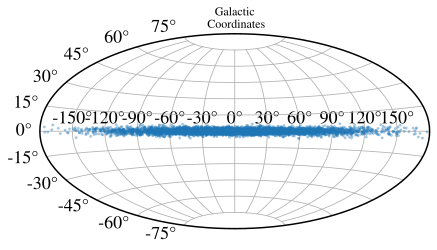
\includegraphics{index_files/mediabag/chap1_files/figure-pdf/gal-eq-output-2.pdf}

}

\caption{Galaxy in Galactic Coordiantes}

\end{figure}%

Now let's plot it in equatorial coordinates (right ascension,
declination).

\begin{Shaded}
\begin{Highlighting}[]
\ImportTok{from}\NormalTok{ astropy }\ImportTok{import}\NormalTok{ units }\ImportTok{as}\NormalTok{ u}
\ImportTok{from}\NormalTok{ astropy.coordinates }\ImportTok{import}\NormalTok{ SkyCoord}

\NormalTok{c\_gal }\OperatorTok{=}\NormalTok{ SkyCoord(l}\OperatorTok{=}\NormalTok{ll}\OperatorTok{*}\NormalTok{u.radian, b}\OperatorTok{=}\NormalTok{bb}\OperatorTok{*}\NormalTok{u.radian, frame}\OperatorTok{=}\StringTok{\textquotesingle{}galactic\textquotesingle{}}\NormalTok{)}
\NormalTok{c\_gal\_icrs }\OperatorTok{=}\NormalTok{ c\_gal.icrs}
\end{Highlighting}
\end{Shaded}

Because \texttt{matplotlib} needs the coordinates in radians and between
\(-\pi\) and \(\pi\), not 0 and \(2\pi\), we have to convert them.

\begin{Shaded}
\begin{Highlighting}[]
\NormalTok{ra\_rad }\OperatorTok{=}\NormalTok{ c\_gal\_icrs.ra.wrap\_at(}\DecValTok{180} \OperatorTok{*}\NormalTok{ u.deg).radian}
\NormalTok{dec\_rad }\OperatorTok{=}\NormalTok{ c\_gal\_icrs.dec.radian}

\NormalTok{plt.figure(figsize}\OperatorTok{=}\NormalTok{(}\DecValTok{7}\NormalTok{,}\DecValTok{5}\NormalTok{))}
\NormalTok{ax }\OperatorTok{=}\NormalTok{ plt.subplot(}\DecValTok{111}\NormalTok{, projection}\OperatorTok{=}\StringTok{"mollweide"}\NormalTok{)}
\NormalTok{ax.set\_title(}\StringTok{"Equatorial coordinates"}\NormalTok{)}
\NormalTok{plt.grid(}\VariableTok{True}\NormalTok{)}
\NormalTok{ax.plot(ra\_rad, dec\_rad, }\StringTok{\textquotesingle{}o\textquotesingle{}}\NormalTok{, markersize}\OperatorTok{=}\DecValTok{2}\NormalTok{, alpha}\OperatorTok{=}\FloatTok{0.3}\NormalTok{)}
\NormalTok{plt.show()}
\CommentTok{\#NOTE: Normally right ascension is plotted from right (0 deg.) to left (360 deg.)}
\end{Highlighting}
\end{Shaded}

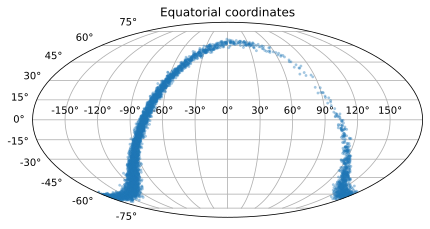
\includegraphics{index_files/mediabag/chap1_files/figure-pdf/cell-10-output-1.pdf}

\section*{Special Relativity}\label{special-relativity}
\addcontentsline{toc}{section}{Special Relativity}

\markright{Special Relativity}

\subsection*{Introduction}\label{introduction}
\addcontentsline{toc}{subsection}{Introduction}

Why is it important?

\[\gamma = \sqrt{\frac{1}{1-\beta^2}}\;, \beta = \frac{v}{c}\]

\begin{itemize}
\tightlist
\item
  Jets emitted by supermassive black holes have:
  \(\gamma \approx 30 \rightarrow \beta = 0.9984\)
\item
  Electrons spiraling in B-field lines of pulsars have:
  \(\gamma \sim 10^7\)
\item
  Lorentz factors of protons of \(10^{20}\) eV:
  \(\gamma = \frac{E}{m^0_p c^2} = \frac{10^{20}}{1\times 10^9} = 10^{11}\)
\end{itemize}

Two principles:

\begin{enumerate}
\def\labelenumi{\arabic{enumi}.}
\item
  \emph{The Principle of Relativity} -- The laws by which the states of
  physical systems undergo change are not affected, whether these
  changes of state be referred to the one or the other of two systems in
  uniform translatory motion relative to each other
\item
  \emph{The Principle of Invariant Light Speed}-- ``\ldots{} light is
  always propagated in empty space with a definite velocity {[}speed{]}
  c which is independent of the state of motion of the emitting body.''
\end{enumerate}

\subsection*{Lorentz Transformations}\label{lorentz-transformations}
\addcontentsline{toc}{subsection}{Lorentz Transformations}

As a simple case, consider a reference frame \emph{O} and and observer
in another frame \emph{O'} moving at constant speed \(\beta\) along the
\(x\) axis:

\begin{figure}[H]

{\centering \includesvg{index_files/mediabag/Frames_of_reference_.svg}

}

\caption{Source: Wikipedia}

\end{figure}%

A Lorentz transformation or \emph{boost} is the transformation from one
inertial reference frame to another. In general it is a \((4\times4)\)
matrix which encapsulates the system of equations describing the
transformation (in natural units).

\[\begin{aligned}
t' &= \gamma(t - \beta x) \\
x' &= \gamma(x - \beta t) \\
y' &= y \\
z' &= z
\end{aligned}\]

The matrix form of this transformation is

\[x'^\mu = {\Lambda^\mu}_\nu x^\nu, \; {\Lambda^\mu}_\nu =
\begin{pmatrix}
\gamma & -\beta\gamma & 0 & 0 \\
-\beta\gamma & \gamma & 0 & 0 \\
0 & 0 & 1 & 0 \\
0 & 0 & 0 & 1
\end{pmatrix}\]

This is just a particular case of a Lorentz transformation (there is
nothing special on the x-axis) and a variable invariant under a Lorentz
transformation is called \emph{Lorentz invariant or scalar}.

The line element \(\Delta s^2\) is a Lorentz invariant:

\[\Delta s^2 = \Delta t^2 - \Delta x^2 - \Delta y^2 -\Delta z^2 \]

This can be rewritten as the inner product of a 4-vector \(x^{\mu}\):

\[\Delta s^2 = x^2 \equiv x^\mu x_\mu = g_{\mu\nu} x^\mu x^\nu\]

where \emph{metric tensor} \(g_{\mu\nu}\) is:

\[g_{00} = + 1, g_{11} = g_{22} = g_{33} = - 1 , g_{\mu\nu} = 0, \;\mathrm{ for}\; \mu \neq\nu\]

is called the \textbf{Minkowski space}

\subsection*{Consequences of Lorentz
transformations}\label{consequences-of-lorentz-transformations}
\addcontentsline{toc}{subsection}{Consequences of Lorentz
transformations}

Lorentz transformation have the following (some of them really bizarre)
consequences:

\begin{itemize}
\tightlist
\item
  \textbf{Relativity of simultaneity.} \(\Delta t' = 0\) in \(O'\)
  doesn't imply \(\Delta t = 0\) in \(O\):
\end{itemize}

\[\Delta t' = \gamma(\Delta t - \beta \Delta x)\]

\begin{itemize}
\tightlist
\item
  \textbf{Time dilatation.} If \(\Delta x = 0\) i.e.~the ticks of one
  clock:
\end{itemize}

\[\Delta t' = \gamma \Delta t\]

\begin{itemize}
\item
  \textbf{Length contraction.} For events satisfying \(\Delta t' = 0\):

  \[\Delta x' = \frac{\Delta x}{\gamma}\]
\item
  \textbf{Equivalence of mass and energy.}
\end{itemize}

In 1905, Einstein gave his first derivation of the mass-energy
equivalence by studing, in different reference frames, the energy
balance of a body emiting electromagnetic radiation. You can replace
\emph{body} with a \emph{cat} and check a quick proof of the mass energy
equivalence in this video:

\begin{figure}

\centering{

\url{https://www.youtube.com/watch?v=hW7DW9NIO9M}

}

\caption{\label{fig-minute}Source: Minute Physics}

\end{figure}%

\section*{Relativistic kinematics}\label{relativistic-kinematics}
\addcontentsline{toc}{section}{Relativistic kinematics}

\markright{Relativistic kinematics}

\subsection*{Four-vectors}\label{four-vectors}
\addcontentsline{toc}{subsection}{Four-vectors}

We saw that position vectors in Minkowski space become 4-vectors with
zeroth component. \(x^0 = t\), identified with time. Likewise momentum
4-vector has \(p^0 = E\):

\[ {\mathbf P} = (E, \vec{p})\]

\[ {\mathbf X} = (t, \vec{x})\]

We saw that the inner product in Minkowski space is invariant under
Lorentz transformations. In this case, the Lorentz invariant is:

\[  s = p_\mu p^{\mu} = m_0^2 = E^2 -{\vec p\cdot \vec p} \rightarrow E^2 = {\vec p\cdot \vec p} +m_0^2\]

which is the \emph{relativistic energy-momentum relationship}.

\[ E = m = \gamma m_0\]

One can derive the expresions for relativistic 3-momentum and kinetic
energy:

\[|{\vec p}|= \beta E\]

\[E_{kin} \equiv E - m_0 = (\gamma -1) m_0\]

\subsection*{Transformation to the Center-of-Momentum Frame
(COM)}\label{transformation-to-the-center-of-momentum-frame-com}
\addcontentsline{toc}{subsection}{Transformation to the
Center-of-Momentum Frame (COM)}

As a concrete example of how 4-vectors aid real calculations, let's take
the classic case of a transformation to the center-of-momentum frame
(COM), that is, a coordinate frame where the total three-momentum
\(\vec p = 0\). In this case the invariant square of a system is equal
to the total COM energy square or:

\[\sqrt{s} = E_{COM}\]

In the case of a two-particle system with particles A and B with
energies \((E_A)\) and \((E_B)\), and 3-momenta \((\vec{p}_A)\) and
\((\vec{p}_B)\):

\[\begin{aligned}{2}
s = p^2 &= (E_A + E_B)^2 - (\vec{p}_A + \vec{p}_B)^2 \\
    &= m_A^2 + m_B^2 + 2E_AE_B - 2(\vec{p}_A \cdot \vec{p}_B)\\
    &= m_A^2 + m_B^2 + 2E_AE_B( 1 - \beta_A\beta_B\cos \theta)\\
    &= E_{COM}^2
\end{aligned}\]

where we used the fact that:
\[\vec{p}_A \cdot \vec{p}_B = |\vec{p}_A ||\vec{p}_B|\cos\theta\]

and

\[ |\vec{p}| = E\beta \]

The energy available for new particle creation is
\(\epsilon = E_{COM} - m_B - m_A\). If \(E_A \gg m_A\) and
\(E_B \gg m_B\) then

\[\epsilon^2 \approx 2 (E_A E_B - \vec{p}_A \vec{p}_B )\]

\subsection*{Fixed-target experiment}\label{fixed-target-experiment}
\addcontentsline{toc}{subsection}{Fixed-target experiment}

If the target particle B is at rest in the laboratory system (as is the
case in accelerator fixed-target experiments or UHE cosmic rays striking
nucleons in the atmosphere, or \ldots) then \((E_B = m_B)\) and
\((\vec{p}_B = 0)\). In this case,

\[E_{COM}^2 = m_A^2 + m_B^2 + 2E_Am_B
\]

which in the ultra-relativistic limit where energies are much higher
than the masses \((E \gg m)\) simplifies to

\[\epsilon = E_{COM} \simeq \sqrt{2m_BE_A}\]

Equivalently, the threshold energy of the beam particle A needed to
produce a particle of mass \((m_*)\) at rest in the boosted frame is:

\[E_{A,\mathrm{thresh}} = \frac{m_*^2}{2m_B}\]

\begin{tcolorbox}[enhanced jigsaw, colframe=quarto-callout-tip-color-frame, opacitybacktitle=0.6, left=2mm, leftrule=.75mm, opacityback=0, colbacktitle=quarto-callout-tip-color!10!white, breakable, bottomrule=.15mm, toprule=.15mm, colback=white, coltitle=black, bottomtitle=1mm, toptitle=1mm, titlerule=0mm, title=\textcolor{quarto-callout-tip-color}{\faLightbulb}\hspace{0.5em}{Example 1: Pion production}, arc=.35mm, rightrule=.15mm]

Considering the photoproduction of pion on a target proton at rest mass:
\[\gamma + p \rightarrow p + \pi^0\]

\[\begin{alignedat}{2}
 \sqrt{s} = \sqrt{m_p^2 + 2E_\gamma m_p} &\geq m_p + m_{\pi^0}\\
m_p^2 + 2 E_\gamma m_p &\geq m_p^2 + m^2_{\pi^0} + 2 m_p^2 m^2_{\pi^0}
\end{alignedat}\]

\[E_\gamma \geq m_{\pi^0} + \frac{m^2_{\pi^0}}{2 m_p} \approx 145 \mathrm{ \; MeV}\]

\end{tcolorbox}

\subsection*{Collider experiment}\label{collider-experiment}
\addcontentsline{toc}{subsection}{Collider experiment}

In the case of a collider experiment where beam particles A and B are
counter-circulating in an accelerator and collide head-on, then

\[{\vec p}_{A}\cdot{\vec p}_{B} = -|{\vec p}_{A}||{\vec p}_{B}|\]

and the equation of the 3-momenta \({\vec p}_A\) becomes

\[
s = E_{COM}^2 = m_A^2 + m_B^2 + 2(E_AE_B + |{\vec p}_{A}||{\vec p}_{B}|) \rightarrow \epsilon^2 \simeq 4E_AE_B
\]

in the relativistic limit where mass can be ignored. This in turn has
the consequence that in a collider experiment the energy available in
the COM to produce new particles rises linearly with beam energy when
\(E_A = E_B\).

Nevertheless, it is still the case that the COM energies probed by
astroparticles exceeds the LHC's reach by a factor of 10!

\begin{tcolorbox}[enhanced jigsaw, colframe=quarto-callout-tip-color-frame, opacitybacktitle=0.6, left=2mm, leftrule=.75mm, opacityback=0, colbacktitle=quarto-callout-tip-color!10!white, breakable, bottomrule=.15mm, toprule=.15mm, colback=white, coltitle=black, bottomtitle=1mm, toptitle=1mm, titlerule=0mm, title=\textcolor{quarto-callout-tip-color}{\faLightbulb}\hspace{0.5em}{Example 2: UHECR protons}, arc=.35mm, rightrule=.15mm]

Consider an UHECR proton at \(E_p = 10^{10}\;\mathrm{ GeV}\) interacting
with a proton (\(m_p = 1 \mathrm{ GeV}\)) at rest in the atmosphere,
what is the energy in the COM frame?

\[E_{COM} = \sqrt{2 m_p^2 + 2 E_p m_p} \simeq 142\;\; \mathrm{ TeV} \]

\end{tcolorbox}

\subsection*{Two-body decay in COM}\label{two-body-decay-in-com}
\addcontentsline{toc}{subsection}{Two-body decay in COM}

The COM is also useful to estimate the energy of two particles from the
decay of a particle with mass \(M\). If a particle A decays into \(m_1\)
and \(m_2\), we have that in the COM the particle A has
\({\vec p_A} = {\vec p_{COM}} = 0\). Then the invariant is given by:

\[ s = M^2 = (E_1 + E_2)^2 -  (\vec{p}_1 + \vec{p}_2)^2 \]

where \({\vec p_1} = -{\vec p_2}\). The energies in the COM are given
by:

\[ M^2 = (E_1 + E_2)^2 \rightarrow M = E_1 + E_2 \]

\[E_1^2 = p_1^2 + m_1^2\;\;\;\mathrm{ and}\;\; E_2^2 = p_2^2 + m_2^2\]

since \(|{\vec p_1}| = |{\vec p_2}|\) we can make the substraction:

\[E_1^2 - E_2^2 = m_1^2 - m_2^2 \rightarrow E_2^2 = E_1^2 - m_1^2 + m_2^2\]

sustituing \(E_2^2\) in \(M^2 = E_1^2 + E_2^2 + 2E_1 E_2\) and using
\(E_2 = M - E_1\) we have:

\[M^2 = E_1^2 + E_1^2 - m_1^2 + m_2^2 + 2E_1(M- E_1) \]
\[M^2 = 2E_1^2 - m_1^2 + m_2^2 - 2E_1^2 + 2E_1M\]

\[E_1 = \frac{1}{2M}(M^2 + m_1^2 - m_2^2)\]

likewise we can prove:

\[E_2 = \frac{1}{2M}(M^2 + m_2^2 - m_1^2)\]

and the momentum:

\[{|\vec p_1|^2} = E_1^2 - m_1^2 = \frac{1}{4M^2}(M^4 - 2M^2(m_1^2 + m_2^2) + (m_1^2 + m_2^2)^2) = {|\vec p_2|^2}\]

Energies and momentums are fixed, the only unknowns are the angles.

\section*{Cosmology}\label{cosmology}
\addcontentsline{toc}{section}{Cosmology}

\markright{Cosmology}

\subsection*{Red-shift}\label{red-shift}
\addcontentsline{toc}{subsection}{Red-shift}

Red-shift is the shift (towards red) in the electromagnetic spectrum and
is defined as:

\[z=\frac{\lambda_{obs} - \lambda_{emit}}{\lambda_{emit}}\]

If a source of the light is moving away from an observer, then redshift
(z \textgreater{} 0) occurs; if the source moves towards the observer,
then blueshift (z \textless{} 0) occurs. This is true for all
electromagnetic waves and is explained by the Doppler effect.
Consequently, this type of redshift is called the \emph{Doppler
redshift}.

\subsection*{Relativistic Redshift}\label{relativistic-redshift}
\addcontentsline{toc}{subsection}{Relativistic Redshift}

\begin{center}
\includegraphics{images/doppler0.png}
\end{center}

The wavefront moves with velocity \(c\), but at the same time the source
moves away with velocity \(v\). Afte a time \(t_s\) the source has
receded \(vt\). The crest of the wave emission is at
\(\lambda+v t_s=ct_s\). The period in the reference system of the source
is given by:

\[t_s = \frac{\lambda}{c-v} = \frac{c}{(c-v)f_s} = \frac{1}{(1-\beta)f_s},\]

Remember that when a reference \(O_s\) was moving at speed \(\beta\)
from a another reference \(O_{o}\), the time relation was:

\[\Delta t_s = \gamma(\Delta t_{o} - \beta \Delta x_{o})\]

Since \(\Delta x_{o} =0\) (we are just measuring when the crest of the
waves arrive), then the time observed \(t_{o}\) in the reference system
O is given:

\[t_o = \frac{t_s}{\gamma},\]

The corresponding observed frequency is
\[f_o = \frac{1}{t_o} = \gamma (1-\beta) f_s = \sqrt{\frac{1-\beta}{1+\beta}}\,f_s\]

The ratio

\[\frac{f_s}{f_o} = \sqrt{\frac{1+\beta}{1-\beta}}\]

is called the \emph{Doppler factor} of the source relative to the
observer.

The corresponding wavelengths are related by

\[\frac{\lambda_o}{\lambda_s} = \frac{f_s}{f_o} = \sqrt{\frac{1+\beta}{1-\beta}}\]

and the resulting redshift

\[z = \frac{\lambda_o - \lambda_s}{\lambda_s} = \frac{f_s - f_o}{f_o}\]

can be written as

\[z = \sqrt{\frac{1+\beta}{1-\beta}} - 1.\]

When interpreted as a relativistic Doppler shift from object receeding
at velocity \(\beta\), this is:

\[\lambda_o = \sqrt{\frac{1+\beta}{1-\beta}}\lambda_s \simeq (1+\beta)\lambda_s\]

In the non-relativistic limit (when \(v \ll c\)) this redshift can be
approximated by \(z \simeq \beta = \frac{v}{c}\) corresponding to the
classical Doppler effect.

\subsection*{Hubble expansion}\label{hubble-expansion}
\addcontentsline{toc}{subsection}{Hubble expansion}

When ploting their redshift (ie speed) as function of distance (measured
with the techniques we saw, parallax, etc.) in 1929 Hubble found a
correlation between redshift and radial distance from Earth:

\begin{center}
\includegraphics{images/unnamed.gif}
\end{center}

\[v = H_0 r, \; H_0 = 72\;\mathrm{ km/s/Mpc}\]

Note that \(H_0\) has only units of time\(^{-1}\) we explicitely write
the other dimensions to better understand its meaning.

But Doppler redshift does not depends on distance! So this not a doppler
redshift but a \textbf{Cosmological redshift}. In this case the redshift
is not due to relative velocities, the photons instead increase in
wavelength and redshift because the spacetime through which they are
traveling is expanding.

But we said that for midly relativistic objects (and galaxies are moving
at midly relativistic speeds) we can approximate \(z \approx \beta\) so
we \emph{can use \(z\) to estimate distances!}:

\[r \simeq \frac{c}{H_0}z \simeq 4000\;\mathrm{ Mpc}\cdot z\]

For small \(v\) over distance \(r\) the \textbf{velocity is proportional
to the distance}. Note that however this only holds only for \emph{small
redshifts!}.

For larger redshifts other relations with the distance need to be
invoked.

\subsubsection*{Age of the Universe (first
approximation)}\label{age-of-the-universe-first-approximation}
\addcontentsline{toc}{subsubsection}{Age of the Universe (first
approximation)}

If we assume that the rate of expansion (ie H) is essentially constant
(it is not!) the age of the Universe can be estimated by this relation:

\[\frac{d r}{dt} = H_0 r \rightarrow \int \frac{1}{r}dr =\int H_0 dt\]

\[ \mathrm{ In} r = H_0 t \rightarrow r = e^{H_0 t}\]

where Universe increases by a factor \(e\) every
\(t_{\mathrm{Hubble}} = \frac{1}{H_0} = 14\times 10^9\mathrm{ yr}\)
which is the \textbf{Hubble time}.

\subsubsection*{Are we expanding?}\label{are-we-expanding}
\addcontentsline{toc}{subsubsection}{Are we expanding?}

\begin{quote}
\href{https://www.youtube.com/watch?v=5U1-OmAICpU}{Brooklyn is not
expanding!} \emph{Annie Hall}
\end{quote}

\section*{Cosmological principle}\label{cosmological-principle}
\addcontentsline{toc}{section}{Cosmological principle}

\markright{Cosmological principle}

The \emph{cosmological principle} is the notion that the distribution of
matter in the Universe is \textbf{homogeneous} and \textbf{isotropic}
when viewed on a large enough scale.

\begin{itemize}
\tightlist
\item
  \textbf{Homogeneity} states that the distribution of matter is even in
  each epoch.
\item
  \textbf{Isotropy} states that there are no prefered directions in the
  distribution of matter in space.
\end{itemize}

\begin{center}
\includegraphics{index_files/mediabag/2df_slice_blue_big.gif}
\end{center}

The
\href{http://en.wikipedia.org/wiki/Observable_universe\#End_of_Greatness}{End
of Greatness} is an observational scale discovered at roughly 100 Mpc
where the lumpiness seen in the large-scale structure of the universe is
homogenized and isotropized, this together with the isotropy of the CMB
reinforced the idea of the \textbf{Cosmological Principle}.

However, in 2013 a new structure \textbf{3 Gpc} wide has been
discovered, the \href{http://arxiv.org/abs/1311.1104}{Hercules--Corona
Borealis Great Wall}, which puts doubt on the validity of the
cosmological principle\ldots{}

\subsection*{Friedmann--Lemaître-Robertson-Walker}\label{friedmannlemauxeetre-robertson-walker}
\addcontentsline{toc}{subsection}{Friedmann--Lemaître-Robertson-Walker}

Despite seing all galaxies receding, we are not at the center of the
Universe. The common interpretation of the expansion is that we are
living in a Universe that can be thought of lying on the surface of a
balloon. Distances between objects (points on the ballon) on this
manifold are expressed as:

\[r(t) = R(t)r_0\]

where \(R(t)\) is a scale factor, depending on the time, and \(r_0\) is
a \emph{comoving coordinate} without time dependence or current distance
if we assume \(R(0) = 1\), but sometimes its better to explicitelly use
a \emph{normalized} scale factor as \(a(t) = R(t)/R(0)\)

So we are looking for a Universe that is isotropic, homogeneous and it
is expanding. The metric that describes such a Universe is given by the
\textbf{Friedmann--Lemaître-Robertson-Walker} metric:

\[ds^2 = dt^2 - R(t)^2 d \Sigma(k)^2 \]
\[= dt^2 - a^2(t)R^2_0\left[\frac{dr^2}{1 - kr^2} + r^2(d\theta^2  + sin^2\theta d\phi^2)\right]\]

where \(d\Sigma(k)\) refers to the spatial 3-dimentional metric
depending on the curvature parameter \(k\) which takes the values +1, 0,
-1, and we used the normalized form of the scale factor
\(a(t) = R(t)/R_0\).

\begin{figure}[H]

{\centering \includegraphics{index_files/mediabag/universe-shape-1024x.jpg}

}

\caption{Source: quantum-bits.org}

\end{figure}%

The evolution of the scale parameter as in the case of wavelength (see
Exercises):

\[a(t) = \frac{1}{1+z}\]

\subsection*{Friedman equations}\label{friedman-equations}
\addcontentsline{toc}{subsection}{Friedman equations}

The dynamics's of the FLRW metric is governed by the Einstein's
equations. Einstein's original field equations are:

\[R_{\mu\nu} - \frac{1}{2}Rg_{\mu\nu} = 8 \pi GT_{\mu\nu}\]

In Newtonian gravity, the source is mass. In special relativity, is a
more general concept called the energy-momemtum tensor, which may be
modeled as a perfect fluid:

\[T_{\mu\nu} = (\rho + p)U_\mu U_\nu + pg_{\mu\nu}\]

were \(U_\mu\) is the fluid four-velocity amd \(\rho\) is an energy
density. The FLRW metric solution to the Einstein equations can be
reduced to the two \textbf{Friedmann equations}:

\[H^2 \equiv \left(\frac{\dot a}{a}\right)^{2} =  \frac{8\pi G}{3}\rho - \frac{kc^{2}}{a^2R^2_0} \]

and

\[\frac{\ddot a}{a} = -\frac{4\pi G}{3}(\rho + 3p)\]

\subsection*{Cosmological Constants}\label{cosmological-constants}
\addcontentsline{toc}{subsection}{Cosmological Constants}

Given the Friedmann equations we can calculate for any value of \(H\)
the critical density such as the geometry is flat (\(k=0\)):

\[\rho_{crit} = \frac{3H^2}{8\pi G}\]

It is convenient to measure the the total energy density in terms of
critical density by introducing the density parameters:

\[\Omega\equiv\frac{\rho}{\rho_{crit}} = \left(\frac{8\pi G}{3H^2}\right)\rho\]

In general the energy density will have contributions of distinct
components so whe can defined:

\[\Omega_i\equiv\frac{\rho_i}{\rho_{crit}} = \left(\frac{8\pi G}{3H^2}\right)\rho_i\]

where \(i\) stands for the different components of the energy density as
we will see later: matter (or dust), radiation, cosmological density,
curvature density.

For the special case of \(a(t_0) = 1\), ie, today, we have the formula:

\[H_0^2\Omega_0 = \frac{8\pi G}{3}\rho_0\]

\subsection*{The cosmological constant}\label{the-cosmological-constant}
\addcontentsline{toc}{subsection}{The cosmological constant}

Einstein was interested in finding \(\dot{a} = 0\) (ie static)
solutions. This can be achieved if \(k= + 1\) and \(\rho\) is
appropriately tuned. But \(\ddot a\) will not vanish in this case.
Einstein therefore modified his equations to:

\[R_{\mu\nu} - \frac{1}{2}Rg_{\mu\nu} + \Lambda g_{\mu\nu}= 8 \pi GT_{\mu\nu}\]

and with this modification the Friedmann equations are:

\[
\begin{aligned}
H^2  &=  \left(\frac{\dot a}{a} \right)^2 = \frac{8\pi G}{3}\rho + \frac{\Lambda}{3} - \frac{kc^{2}}{a^2R^2_0} \\
\frac{\ddot a}{a} &= -\frac{4\pi G}{3}(\rho + 3p) +  \frac{\Lambda}{3}
\end{aligned}
\]

The discovery by Hubble that the Universe is expanding eliminated the
empirical need for a static world. However, we believe that \(\Lambda\)
is actually nonzero, so Einstein was right after all. Assuming that
cosmological constant is due to the vacuum energy, most quantum field
theories predict a \(\Lambda\) that is 120 orders of magnitude larger
than the observational values! this is so-called \textbf{cosmological
constant problem}.

\subsection*{Evolution of the Cosmological
Constants}\label{evolution-of-the-cosmological-constants}
\addcontentsline{toc}{subsection}{Evolution of the Cosmological
Constants}

In general the energy density will have contributions of distinct
components which will evolve differently with the Universe expansion: *
Massive particles with negligible velocities are known in cosmology as
\emph{dust} or simply \emph{matter}. Their density scales as the number
density times their rest mass. Their number density scales as the
inverse of the volume while the rest mass is constant:
\(\rho_M \propto a^{-3}\) * Relativistic particles are known as
\emph{radiation} (although it is not only photons) and their energy
density is the number density times the particle energy, the latter is
proportional to \(a^{-1}\) (as they redshift with expansion) and so:
\(\rho_r \propto a^{-4}\) * Vacuum energy does not change as universe
expand so we can define a
\(\rho_\Lambda \equiv \frac{\Lambda}{8\pi G} \propto a^0\) * It is
useful to pretend that \(-ka^{-2}R_0^{-2}\) represents an effective
\emph{curvature energy density} defining
\(\rho_k \equiv -(3k/8\pi G R^2_0)a^{-2}\).

Given this evolution it is possible to write:

\[ H^2(t) = H^2_0 [\Omega^0_M(1+z)^3 + \Omega^0_r(1+z)^4 + \Omega^0_k(1+z)^2 +\Omega^0_\Lambda]\]

\subsection*{Observational results}\label{observational-results}
\addcontentsline{toc}{subsection}{Observational results}

\begin{itemize}
\item
  There are good reasons to believe that the energy density of radiation
  is much less than matter, as photon contrinute only to
  \(\Omega_r \sim 5 \times 10^{-5}\) mostly in the CMB. Therefore is
  useful to parametrize the universe today as
  \(\Omega_k = 1 - \Omega_M - \Omega_\Lambda\).
\item
  \textbf{Direct measures of the Hubble constant.}. The most reliable
  result on the Hubble constant comes from the
  \href{http://iopscience.iop.org/0004-637X/553/1/47}{Hubble Space
  Telecope Key Project}. They use the Cepheids to obtain distances to 31
  galaxies (They also use Type Ia Supernovae). A recent study with over
  600 Cepheids yielded the number
  \(H_0 = 73.8 \pm 2.4 \mathrm{\;km\;s^{-1}\; Mpc^{-1}}\). The indirect
  measurement from \emph{Planck} Collaboration gives somehow a lower
  value (this discrepancy as well as the comic distance-ladder method
  are under investigation).
\item
  \textbf{Supernovae.} Two major studies, the Supernova Cosmology
  Project and the High-\(z\) Supernova Search Team, found evidence for
  an accelerating Universe. When combined with the CMB data indicating
  flatness (ie
  \(\Omega_k = 0 \rightarrow \Omega_M + \Omega_\Lambda = 1\)), the
  best-fit values were \(\Omega_M \approx 0.3\) and
  \(\Omega_\Lambda \approx 0.7\))
\item
  \textbf{Cosmic Microwave Background.} See next section.
\end{itemize}

\subsection*{Cosmic Microwave
Background}\label{cosmic-microwave-background}
\addcontentsline{toc}{subsection}{Cosmic Microwave Background}

The cosmic microwave background (CMB) is electromagnetic radiation that
remains from the time when photons decoupled from matter shortly after
the recombination of electrons and protons into neutral hydrogen atoms.
Once photons decoupled from matter, they traveled freely through the
universe without interacting with matter. For an observer today this CMB
is observed as a distribution of temperatures (from black body
radiation) at on a two-dimensional sphere. This temperature
distribution, however, was shown to have anisotropies. If we denote
\(\Delta T (\theta, \phi)\) the temperature difference measured in the
direction
(\(\sin\theta \cos \theta, \sin\theta \sin\theta , \cos\theta\)) with
respect to \(T_0 =\) 2.725 K, the average temperature we can decompose
these anisotropies over the bases of spherical harmonics, the so called
\(Y_{\ell m} (\theta, \phi)\), the same way a we can decompose a
function in a curved space over sines and cosines by the Fourier
transform:

\[\frac{\Delta T}{T} = \sum_{\ell m} a_{\ell m} Y_{\ell m} (\theta, \phi)\]

This decomposition tell us the amount of anisotropy at a given the
multipole moment \(\ell\) or angular scale
\(\theta = \frac{180^{\circ}}{\ell}\)

\[C_\ell = \langle |a_{\ell m}|^2 \rangle\]

\begin{figure}[H]

{\centering \includegraphics{index_files/mediabag/Planck_power_spectru.jpg}

}

\caption{Source: ESA}

\end{figure}%

The power spectrum of the CMB represents the anisotropies of the CMB as
a function of the angular scale. The typical spectrum features a plateu
at large angular scales (small \(\ell\)) followed by some oscillatory
features (aka acoustic peaks or \emph{Doppler peak}). These peaks
represent the oscillation of photon-baryon fuild around the decoupling.
The first peak at \(\ell \sim 200\) probes the spatial geometry, while
the relative heights probe the baryon density. The position of the first
peak constrains the spatial geometry in a way consistent with a flat
Universe (\(\Omega_k \sim 0\))

\begin{tcolorbox}[enhanced jigsaw, colframe=quarto-callout-note-color-frame, opacitybacktitle=0.6, left=2mm, leftrule=.75mm, opacityback=0, colbacktitle=quarto-callout-note-color!10!white, breakable, bottomrule=.15mm, toprule=.15mm, colback=white, coltitle=black, bottomtitle=1mm, toptitle=1mm, titlerule=0mm, title=\textcolor{quarto-callout-note-color}{\faInfo}\hspace{0.5em}{Note}, arc=.35mm, rightrule=.15mm]

Build your own Universe
\href{https://lambda.gsfc.nasa.gov/education/cmb_plotter/}{here}

\end{tcolorbox}

\subsection*{Before Planck}\label{before-planck}
\addcontentsline{toc}{subsection}{Before Planck}

\begin{center}
\includegraphics{images/eso0419d.jpg}
\end{center}

\subsection*{After Planck}\label{after-planck}
\addcontentsline{toc}{subsection}{After Planck}

Planck showed that the amount of dark energy in the Universe is
appreciably less than we had previously thought, while the amount of
dark-and-normal matter is appreciably greater than we thought.

\begin{center}
\includegraphics{images/Lambda_Matter.jpg}
\end{center}

\subsection*{Cosmography}\label{cosmography}
\addcontentsline{toc}{subsection}{Cosmography}

Using the Huble equation we are going to derive some quantities related
to the measurement of the Universe.

\subsubsection*{Age of the Universe}\label{age-of-the-universe}
\addcontentsline{toc}{subsubsection}{Age of the Universe}

We have shown the evolution of the Hubble expansion as a function of the
redshift using the clousure parameters. We know that

\[H(z) = \frac{\dot a}{a} = -\left(\frac{\mathrm{ d}z/\mathrm{ d}t}{(1+z)}\right) \rightarrow \mathrm{ d}t = -\frac{\mathrm{ d}z}{(1+z)H(z)}\]

And so the age of the universe can be calculated as (where \(z=0\)
corresponds to today \(t_0\)):

\[\int_{0}^{t_0} \mathrm{ d} t = t_0 = \frac{1}{H_0} \int^\infty_0 \frac{\mathrm{ d}z}{E(z)}\]

where we defined the following function:

\[E(z)\equiv \sqrt{\Omega_M(1+z)^4 + \Omega_r(1+z)^5 + \Omega_k(1+z)^3 +\Omega_\Lambda(1+z)}\]

Assuming a flat Universe \(\Omega_k =0\) and ignoring the radiation
\(\Omega_r \ll \Omega_M\) the integral gets simplified to:

\[H_0 t_0 = \frac{1}{3\sqrt{1 - \Omega_M}}\mathrm{ In}\left(\frac{1+\sqrt{1 - \Omega_M}}{1 - \sqrt{1- \Omega_M}}\right)\]
where we used \(1 = \Omega_\Lambda + \Omega_M\)

For \(\Omega_M = 0.70\) and \(\Omega_\Lambda = (1 - \Omega_M) = 0.30\)
one finds \(H_0 t_0 = 0.964\) so that
\(t_0 \approx \frac{0.96}{H_0} = 13.5\) Gyr. Which is similar to the
assumption we did with a constant \(H_0\).

\subsubsection*{Comoving distance (Line of
Sight)}\label{comoving-distance-line-of-sight}
\addcontentsline{toc}{subsubsection}{Comoving distance (Line of Sight)}

The comoving distance between two nearby objects in the Universe is the
distance between them which remains constant with epoch if the two
objects are moving with the \emph{Hubble flow}. That an object follows
the \emph{Hubble flow} if there is no peculiar velocities, ie, the only
reason the 2 objects separate is due to the expansion of the Universe
and not because the have relative velocities among them. The comoving
distance has the expansion factored out and therefore remains constant
with epoch. You can think of it as the distance measured with a ruler
that also expands with the Universe. Using the same argument as above
with the age of the Universe we can multiplying by the speed of light we
can derive:

\[D_c(z) = \int_{t}^{t_0} c\mathrm{ d} t = \frac{c}{H_0} \int^z_0 \frac{\mathrm{ d}z^\prime}{E(z^\prime)}.\]

This is the comoving distance along the \emph{line of sight}. Ie, is the
comoving distance from a galaxy at redshift \(z\) from us. If we want to
estimate, let's say, the distance between 2 galaxies at the same
redshift but separated in angle \(\Delta \theta\), then the distance is
given by \(D_M \Delta \theta\) where \(D_M\) is the \emph{transverse
comoving distance}. For a flat Universe \(D_M = D_c\) but if the
curvature is not zero, the relationship depends on the trigonometric
functions \(\sinh\) (for a closed Universe) and \(\sin\) (for an open
Universe) to account for the curvature of spacetime.

\subsubsection*{Luminosity distances}\label{luminosity-distances}
\addcontentsline{toc}{subsubsection}{Luminosity distances}

The luminosity distance defined in cosmology is defined as the distace
in which an object with intrinsic luminosity \(L\) is observed with flux
\(f\), ie:

\[ f = \frac{L}{4\pi d_L^2}\]

This in terms of bolometric values, however sometimes we only observe a
given bandwidth in frequency, ie, we have to replace
\(f\rightarrow f(\nu_o)\) and \(L \rightarrow L(\nu_{e})\) where
\(\nu_o\) and \(\nu_e\) are the observed and emitted frequencies. Since
the luminosity is defined as energy delivered over interval of time, we
can approximate it as:

\[ L(\nu_e) = \frac{Nh\nu_e}{\Delta t_e},\]
\[ L(\nu_o) = \frac{Nh\nu_o}{\Delta t_o},\]

being \(N\) the number of photos. However the photons emitted are
redshifted and photons observed at \(\nu_o\) were emitted at
\((1+z)\nu_o\). The time intervals are also related by the expansion of
the Universe as:

\[\frac{\Delta t_e}{\Delta t_o} = \frac{1}{(1+z)}\]

So we have that the emitted luminosity and the observed luminosity are
related as:

\[L(\nu_o) = \frac{L(\nu_e)}{(1+z)^2}\]

The observed luminosity is smaller than the emitted luminosity. On the
other hand the relation between the observed flux and observed
luminosity is the same as in a non-expanding Universe. ie:

\[f(\nu_o) = \frac{L(\nu_o)}{4\pi D_c^2},\]

where \(D_c\) is the co-moving distance. Putting everything together we
have that:

\[f(\nu_o) = \frac{1}{(1+z)^2}\frac{L(\nu_e)}{4\pi D_c^2} = \frac{L(\nu_e)}{4\pi D_L^2}\]
so we have the relation between the luminosity distance and the
co-moving distance as:

\[D_L = D_c(1+z)\]

\subsection*{Tutorial III: Age of the
Universe}\label{tutorial-iii-age-of-the-universe}
\addcontentsline{toc}{subsection}{Tutorial III: Age of the Universe}

In the about the age of the Universe we calculated an analytical
solution for a given condition. No we are goign to use \texttt{python}
to numerically solve the look-back time for any given set of
cosmological parameters. For that we are going to rewrite the loopback
formula in terms of the scale factor \(a\) since we have the redshift
scale relation:

\[(1+z) = \frac{1}{a}\]

we can prove that:

\[\frac{\mathrm{ d}z}{1 +z} = -\frac{\mathrm{ d}a}{a}\]

Therefore the equation above that relates \(\mathrm{d}t\) with redshift
we can rewrite it at:

\[ \mathrm{ d}t = \frac{\mathrm{d}a}{H(a)a} \]

with

\[  H^2(a) = H^2_0 [\Omega^0_M a^{-3} + \Omega^0_r a^{-4} + \Omega^0_k a^{-2} +\Omega^0_\Lambda] \]

We need to numerically integrate the right hand side of the equation.
However, for some parameters this integration is circular, reaching a
\(a_{max}\) then the \(H^2(a_{max}) = 0\)

\begin{Shaded}
\begin{Highlighting}[]
\CommentTok{\#We take the current value of H0 from the astropy package}

\ImportTok{from}\NormalTok{ astropy.cosmology }\ImportTok{import}\NormalTok{ Planck13}
\NormalTok{H0 }\OperatorTok{=}\NormalTok{ Planck13.H(}\DecValTok{0}\NormalTok{).value}

\CommentTok{\#We define the friedman equation ignoring the radiation component omega\_r \textless{}\textless{}}
\KeywordTok{def}\NormalTok{ friedman(a, omega\_M, omega\_lambda):}
\NormalTok{    omega\_k }\OperatorTok{=} \DecValTok{1} \OperatorTok{{-}}\NormalTok{ omega\_M }\OperatorTok{{-}}\NormalTok{ omega\_lambda}
\NormalTok{    H2 }\OperatorTok{=}\NormalTok{ H0}\OperatorTok{**}\DecValTok{2} \OperatorTok{*}\NormalTok{ (omega\_M }\OperatorTok{*}\NormalTok{ a}\OperatorTok{**{-}}\DecValTok{3} \OperatorTok{+}\NormalTok{ omega\_k }\OperatorTok{*}\NormalTok{ a}\OperatorTok{**{-}}\DecValTok{2} \OperatorTok{+}\NormalTok{ omega\_lambda)}
    \ControlFlowTok{return}\NormalTok{ H2}

\ImportTok{import}\NormalTok{ scipy.integrate }\ImportTok{as}\NormalTok{ integrate}

\CommentTok{\#This is a simple integration, it does not take into account a possible Big Crunch}
\CommentTok{"""}
\CommentTok{def calculate\_times(omega\_m, omega\_lambda):}
\CommentTok{    t0 = integrate.quad(lambda x: 1/x * 1/np.sqrt(friedman(x,omega\_m, omega\_lambda)), 0, 1)[0]}
\CommentTok{    times = []}
\CommentTok{    scales = np.arange(0.1, 2, 0.01)}
\CommentTok{    for a in scales:}
\CommentTok{        time = integrate.quad(lambda x: 1/x * 1/np.sqrt(friedman(x,omega\_m, omega\_lambda)), 0, a)[0]}
\CommentTok{        times.append(H0*(time {-} t0))  }

\CommentTok{    return np.array(times), np.array(scales)}
\CommentTok{"""}

\CommentTok{\#This integration takes into account a Big Crunch}
\KeywordTok{def}\NormalTok{ calculate\_times(omega\_m, omega\_lambda):}
    \CommentTok{\#Lets check if there is a maximal, ie, if H\^{}2(a) = 0}
\NormalTok{    astep }\OperatorTok{=} \FloatTok{0.001}
\NormalTok{    amax }\OperatorTok{=} \DecValTok{3}
\NormalTok{    scales }\OperatorTok{=}\NormalTok{ np.arange(}\FloatTok{0.1}\NormalTok{, amax, astep)}

\NormalTok{    f }\OperatorTok{=}\NormalTok{ friedman(scales, omega\_m, omega\_lambda)}
\NormalTok{    ia, }\OperatorTok{=}\NormalTok{ np.where(np.diff(np.sign(f)))}

    \ControlFlowTok{if} \BuiltInTok{len}\NormalTok{(ia) }\OperatorTok{!=} \DecValTok{0}\NormalTok{:}
\NormalTok{        amax }\OperatorTok{=}\NormalTok{ scales[ia[}\DecValTok{0}\NormalTok{]]}
    
\NormalTok{    tmax }\OperatorTok{=}\NormalTok{ integrate.quad(}\KeywordTok{lambda}\NormalTok{ x: }\DecValTok{1}\OperatorTok{/}\NormalTok{x }\OperatorTok{*} \DecValTok{1}\OperatorTok{/}\NormalTok{np.sqrt(friedman(x,omega\_m, omega\_lambda)), }\DecValTok{0}\NormalTok{, amax }\OperatorTok{{-}}\NormalTok{ astep)[}\DecValTok{0}\NormalTok{]}
    \CommentTok{\#time today a = 1}
\NormalTok{    t0 }\OperatorTok{=}\NormalTok{ integrate.quad(}\KeywordTok{lambda}\NormalTok{ x: }\DecValTok{1}\OperatorTok{/}\NormalTok{x }\OperatorTok{*} \DecValTok{1}\OperatorTok{/}\NormalTok{np.sqrt(friedman(x,omega\_m, omega\_lambda)), }\DecValTok{0}\NormalTok{, }\DecValTok{1}\NormalTok{)[}\DecValTok{0}\NormalTok{]}

    \CommentTok{\#Empty x,y for the plots}
\NormalTok{    times }\OperatorTok{=}\NormalTok{ []}
\NormalTok{    scale }\OperatorTok{=}\NormalTok{ []}
    \ControlFlowTok{for}\NormalTok{ a }\KeywordTok{in}\NormalTok{ scales:}
        \ControlFlowTok{if}\NormalTok{ a }\OperatorTok{\textless{}}\NormalTok{ amax: }\CommentTok{\#If a \textless{} amax we do the typical integral 0 {-}\textgreater{} a}
\NormalTok{            time }\OperatorTok{=}\NormalTok{ integrate.quad(}\KeywordTok{lambda}\NormalTok{ x: }\DecValTok{1}\OperatorTok{/}\NormalTok{x }\OperatorTok{*} \DecValTok{1}\OperatorTok{/}\NormalTok{np.sqrt(friedman(x,omega\_m, omega\_lambda)), }\DecValTok{0}\NormalTok{, a)[}\DecValTok{0}\NormalTok{]}
\NormalTok{            times.append(H0}\OperatorTok{*}\NormalTok{(time }\OperatorTok{{-}}\NormalTok{ t0)) }\CommentTok{\#We calibrate at {-}t0 to place all curves together}
\NormalTok{            scale.append(a)}
        \ControlFlowTok{if}\NormalTok{ a }\OperatorTok{\textgreater{}=}\NormalTok{ amax }\KeywordTok{and} \DecValTok{2}\OperatorTok{*}\NormalTok{amax }\OperatorTok{{-}}\NormalTok{ a }\OperatorTok{\textgreater{}} \DecValTok{0}\NormalTok{: }\CommentTok{\#If a \textgreater{} amax we are out the domain we integrate backwards}
\NormalTok{            time }\OperatorTok{=} \DecValTok{2}\OperatorTok{*}\NormalTok{tmax }\OperatorTok{{-}}\NormalTok{ integrate.quad(}\KeywordTok{lambda}\NormalTok{ x: }\DecValTok{1}\OperatorTok{/}\NormalTok{x }\OperatorTok{*} \DecValTok{1}\OperatorTok{/}\NormalTok{np.sqrt(friedman(x,omega\_m, omega\_lambda)), }\DecValTok{0}\NormalTok{, }\DecValTok{2}\OperatorTok{*}\NormalTok{amax }\OperatorTok{{-}}\NormalTok{ a)[}\DecValTok{0}\NormalTok{]}
\NormalTok{            times.append(H0}\OperatorTok{*}\NormalTok{(time }\OperatorTok{{-}}\NormalTok{ t0))}
\NormalTok{            scale.append(}\DecValTok{2}\OperatorTok{*}\NormalTok{amax }\OperatorTok{{-}}\NormalTok{ a)}
    \ControlFlowTok{return}\NormalTok{ np.array(times), np.array(scale)}

\NormalTok{fig, ax }\OperatorTok{=}\NormalTok{ plt.subplots(}\DecValTok{1}\NormalTok{, }\DecValTok{1}\NormalTok{, figsize}\OperatorTok{=}\NormalTok{(}\DecValTok{5}\NormalTok{,}\DecValTok{4}\NormalTok{))}

\NormalTok{omega\_M }\OperatorTok{=} \FloatTok{0.3}
\NormalTok{omega\_lambda }\OperatorTok{=} \FloatTok{0.7}
\NormalTok{x, y }\OperatorTok{=}\NormalTok{ calculate\_times(omega\_M, omega\_lambda)}
\NormalTok{ax.plot(x, y, label}\OperatorTok{=}\VerbatimStringTok{fr"$\textbackslash{}Omega\_M =$ }\SpecialCharTok{\{}\NormalTok{omega\_M}\SpecialCharTok{:.2f\}}\VerbatimStringTok{, $\textbackslash{}Omega\_\textbackslash{}Lambda =$ }\SpecialCharTok{\{}\NormalTok{omega\_lambda}\SpecialCharTok{:.2f\}}\VerbatimStringTok{"}\NormalTok{)}

\NormalTok{omega\_M }\OperatorTok{=} \FloatTok{1.0}
\NormalTok{omega\_lambda }\OperatorTok{=} \DecValTok{0}
\NormalTok{x, y }\OperatorTok{=}\NormalTok{ calculate\_times(omega\_M, omega\_lambda)}
\NormalTok{ax.plot(x, y, lw }\OperatorTok{=} \DecValTok{2}\NormalTok{, label}\OperatorTok{=}\VerbatimStringTok{fr"$\textbackslash{}Omega\_M =$ }\SpecialCharTok{\{}\NormalTok{omega\_M}\SpecialCharTok{:.2f\}}\VerbatimStringTok{, $\textbackslash{}Omega\_\textbackslash{}Lambda =$ }\SpecialCharTok{\{}\NormalTok{omega\_lambda}\SpecialCharTok{:.2f\}}\VerbatimStringTok{"}\NormalTok{)}

\NormalTok{omega\_M }\OperatorTok{=} \FloatTok{0.3}
\NormalTok{omega\_lambda }\OperatorTok{=} \DecValTok{0}
\NormalTok{x, y }\OperatorTok{=}\NormalTok{ calculate\_times(omega\_M, omega\_lambda)}
\NormalTok{ax.plot(x, y, lw }\OperatorTok{=} \DecValTok{2}\NormalTok{, label}\OperatorTok{=}\VerbatimStringTok{fr"$\textbackslash{}Omega\_M =$ }\SpecialCharTok{\{}\NormalTok{omega\_M}\SpecialCharTok{:.2f\}}\VerbatimStringTok{, $\textbackslash{}Omega\_\textbackslash{}Lambda =$ }\SpecialCharTok{\{}\NormalTok{omega\_lambda}\SpecialCharTok{:.2f\}}\VerbatimStringTok{"}\NormalTok{)}

\NormalTok{omega\_M }\OperatorTok{=} \DecValTok{4}
\NormalTok{omega\_lambda }\OperatorTok{=} \DecValTok{0}
\NormalTok{x, y }\OperatorTok{=}\NormalTok{ calculate\_times(omega\_M, omega\_lambda)}
\NormalTok{ax.plot(x, y, lw }\OperatorTok{=} \DecValTok{2}\NormalTok{, label}\OperatorTok{=}\VerbatimStringTok{fr"$\textbackslash{}Omega\_M =$ }\SpecialCharTok{\{}\NormalTok{omega\_M}\SpecialCharTok{:.2f\}}\VerbatimStringTok{, $\textbackslash{}Omega\_\textbackslash{}Lambda =$ }\SpecialCharTok{\{}\NormalTok{omega\_lambda}\SpecialCharTok{:.2f\}}\VerbatimStringTok{"}\NormalTok{)}


\NormalTok{plt.legend(loc}\OperatorTok{=}\StringTok{"upper left"}\NormalTok{)}
\NormalTok{ax.grid()}
\NormalTok{ax.set\_xlim(}\OperatorTok{{-}}\DecValTok{1}\NormalTok{,}\FloatTok{1.5}\NormalTok{)}
\NormalTok{ax.set\_ylim(}\FloatTok{0.2}\NormalTok{,}\DecValTok{2}\NormalTok{)}
\NormalTok{ax.set\_ylabel(}\StringTok{"$a(t)$"}\NormalTok{)}
\NormalTok{ax.set\_xlabel(}\StringTok{"$H\_0 (t {-} t\_0)$"}\NormalTok{)}
\NormalTok{plt.show()}
\end{Highlighting}
\end{Shaded}

\begin{figure}[H]

\centering{

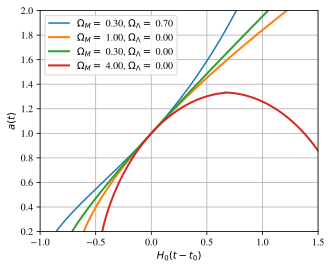
\includegraphics{index_files/mediabag/chap1_files/figure-pdf/fig-age-output-1.pdf}

}

\caption{\label{fig-age}Age of the Universe}

\end{figure}%

\subsubsection*{References}\label{references}
\addcontentsline{toc}{subsubsection}{References}

\phantomsection\label{refs}
\begin{CSLReferences}{0}{1}
\end{CSLReferences}

\bookmarksetup{startatroot}

\chapter*{Cosmic Rays}\label{cosmic-rays}
\addcontentsline{toc}{chapter}{Cosmic Rays}

\markboth{Cosmic Rays}{Cosmic Rays}

\section*{What are Cosmic Rays? An historic
perspective}\label{what-are-cosmic-rays-an-historic-perspective}
\addcontentsline{toc}{section}{What are Cosmic Rays? An historic
perspective}

\markright{What are Cosmic Rays? An historic perspective}

To explain cosmic rays, we need to go back about 100 years to the year
1912 when Victor Hess concluded a series of balloon flights equipped
with an electroscope. He measured how ionization in the atmosphere
increased as he moved away from the Earth's surface. The origin of this
ionization had to be some type of radiation, and since it increased with
altitude, the origin couldn't be terrestrial. In other words, there
existed, and still exists, radiation coming from outer space. For this
milestone, Victor Hess is known as the discoverer of cosmic rays.
However, it would be unfair to attribute the merit solely to Hess, as
many physicists before him had already paved the way that would
culminate in his famous balloon flights: Theodor Wulf, Karl Bergwitz,
and Domenico Pacini, among others, laid the foundations for one of the
branches of particle physics that would dominate the field for the next
40 years until the advent of the first particle accelerators in the
early 1950s.

\begin{figure}[H]

{\centering \includegraphics{images/Electroscope_showing_induction.png}

}

\caption{Source: Sylvanus P. Thompson (1881) Elementary Lessons in
Electricity and Magnetism, MacMillan, New York, p.16, fig.~12}

\end{figure}%

From the begining, cosmic rays were mysterious: What was their origin?
What were these ionizing rays? During the 1920s, Bruno Rossi and Robert
Millikan engaged in a lively debate on the nature of cosmic rays.
Millikan proposed that cosmic rays were ``ultra''-gamma rays, photons of
very high energy created in the fusion of hydrogen in space. Rossi's
measurements, showing an East-West asymmetry in the intensity of cosmic
rays, suggested instead that cosmic rays must be charged particles,
disproving Millikan's theories. There is a famous anecdote in which
Rossi, during the introductory talk at a conference in Rome, said:
\textgreater{} Clearly, Millikan is resentful because a young man like
me has shattered his beloved theory, so much so that from that moment
on, he refuses to acknowledge my existence'' A hundred years later, we
know that Rossi was indeed correct. The majority, 90\%, of cosmic rays
are protons and other heavy nuclei. The ratio of nuclei faithfully
follows the atomic abundance found in our Solar System, indicating that
the origin of these particles is stellar. There are some exceptions; for
example, lithium, beryllium, and boron are nuclei that we can find among
cosmic rays in a proportion greater than in our environment. These
nuclei are actually produced by the fragmentation of heavier ones, such
as carbon, during their journey through space. Thus, the abundance ratio
between carbon and boron provides information about how long carbon has
been traveling through space.

The spectrum, or the number of particles per unit area and time as a
function of energy, has also been measured in great detail over the last
30 years thanks to the work of numerous experiments. The cosmic ray
spectrum is remarkable in both its variation and energy range. The
number of particles, or flux, covers 32 orders of magnitude, so we find
that the least energetic particles reach Earth at a rate of one particle
per square meter every second. On the other hand, the most energetic
ones arrive at a rate of one particle per square kilometer per year.
This is why physicists have had to develop various experimental
techniques to measure the spectrum of cosmic rays in its entirety: from
particle detectors sent into space on satellites or attached to the
International Space Station, to experiments deployed on large surfaces
of the Earth to detect the most energetic cosmic rays, such as the
Pierre Auger Observatory covering an area of about 3000 km2 on the high
plateau of the Pampa Amarilla in Malargüe, Argentina.

But what makes cosmic rays truly fascinating is the amount of energy
these particles can reach, far superior to what can be achieved today
with the most powerful accelerator built by humans with the Large Hadron
Collider (LHC) at the European Organization for Nuclear Research (CERN)
in Geneva. The LHC is an underground ring with a length of 27 km located
on the Franco-Swiss border near Geneva, Switzerland, using powerful
magnets to accelerate protons to 99.99\% of the speed of light. Despite
the impressiveness of this experiment, if we were to accelerate
particles to the energies of cosmic rays with the same technology, we
would need an accelerator the size of the orbit of Mercury. The speed of
cosmic rays is so high that the effects of space-time relativity are
considerable. For example, although the radius of our Galaxy is about
100,000 light-years, due to the temporal contraction of special
relativity, the most energetic cosmic rays would experience they will
experience the journey in just 10 seconds. When cosmic rays reach Earth,
they encounter 10 kilometers of atmosphere which, along with the Earth's
magnetic field, fortunately acts as a shield and protects us from
radiation. However, when cosmic rays collide with atoms in the
atmosphere, they trigger a shower of new particles. This shower is known
as secondary cosmic rays, and in it, we can find a diverse array of new
particles. This is why, for many years, the physics of cosmic rays was
the only way for particle physicists to discover and study new
particles. Thus, following in Hess's footsteps, during the 1940s, many
physicists moved from the laboratory to hot air balloons equipped with
bubble chambers (a primitive version of a particle detector) to study
this myriad of new particles. Among the new particles discovered were,
for example, the first particle of antimatter: the positron, a
positively charged electron, as well as the muon, with properties
similar to the electron but with greater mass.

But what is the origin of cosmic rays? Which sources in the Universe are
capable of accelerating particles to such energies? That is the question
that, despite 100 years since Victor Hess's discovery, physicists have
not been able to fully answer. The main reason is, however, easy to
understand. Cosmic rays, being charged particles, are deflected by
magnetic fields during their journey through the Universe. Both the
Milky Way and intergalactic space are immersed in magnetic fields, so
when cosmic rays reach Earth, their direction has little or nothing to
do with the original direction, making it impossible to do
\emph{astronomy}. However, despite this disadvantage, we can deduce some
things about their origin based on, for example, their energy. We know
that low-energy cosmic rays must come from our own Galaxy because the
magnetic fields of the Milky Way would confine them until they
eventually interact with Earth. On the other end of the spectrum,
extremely high-energy cosmic rays (UHECRs) must come from outside our
own Galaxy since they are so energetic that the magnetic fields of their
respective galaxies would not be able to retain them. The exact turning
point in energy between these two origins is uncertain. So far, we have
been unable to undoubtivously observe a cosmic-ray source. One of the
main candidates for the source of galactic cosmic rays are supernova
remnants. At the end of a star's life cycle, it can explode, releasing a
large amount of mass and energy. What remains behind can be a neutron
star surrounded by all the remnants left from the original star; this is
what is called a supernova remnant. It is more challenging to conceive a
cosmic accelerator capable of accelerating particles up to the energy
equivalent of a soccer ball kicked at 50 km/h, which corresponds to the
energies of UHECRs. Here the list of candidates is considerably reduced
because there are fewer objects in the Universe with the magnetic field
and size sufficient to act as a large particle accelerator. The
candidates are active galactic nuclei and gamma-ray bursts. Active
galactic nuclei are the nuclei of galaxies with a supermassive black
hole at their center. These nuclei show beams of particles in opposite
directions that could function as large accelerators. On the other hand,
gamma-ray bursts are the most violent events known in the Universe, and
their origin and nature would warrant another chapter of this book.
Lasting from a few seconds to a few minutes, these events can illuminate
the entire sky by releasing their energy mainly in the form of very
high-energy photons. But if cosmic rays never point to their source, how
can we ever be sure that active galactic nuclei or gamma-ray bursts are
the true sources of cosmic rays? To answer this puzzle, we need what has
been dubbed as \emph{multi-messenger astronomy}. Thanks to particle
physics, we know that under the conditions in which, for example, a
proton is accelerated to high energies, reactions with the surrounding
matter can occur. These interactions would produce other particles such
as very high-energy photons and neutrinos. Neutrinos are especially
interesting because they are not only neutral and therefore travel in a
straight line without being deflected by magnetic fields, but they are
also weakly interacting particles, so unlike photons, they can traverse
dense regions of the Universe without being absorbed. Future multi
messenger experiments will be able to solve the mystery of cosmic rays.

\section*{The Cosmic Ray Spectrum}\label{the-cosmic-ray-spectrum}
\addcontentsline{toc}{section}{The Cosmic Ray Spectrum}

\markright{The Cosmic Ray Spectrum}

Cosmic rays mostly protons accelerated at sites within the galaxy.

\begin{itemize}
\tightlist
\item
  As they are charged they are deviated in galactic and inter-galactic
  \(\vec{B}\) and solar and terrestrial magnetic fields. Directionality
  only possible for \(E \gt 10^{19}\) eV.
\item
  But interactions with CMB at \(E \sim 10^{19}\) limit horizon tens or
  hundreds of Mpc.
\item
  One century after discovery, origins of cosmic rays, in particular
  UHECR, remain \textbf{unknown}
\end{itemize}

\begin{Shaded}
\begin{Highlighting}[]
\ImportTok{import}\NormalTok{ crdb}
\ImportTok{import}\NormalTok{ matplotlib.pylab }\ImportTok{as}\NormalTok{ plt}
\ImportTok{import}\NormalTok{ numpy }\ImportTok{as}\NormalTok{ np}

\ImportTok{from}\NormalTok{ crdb.experimental }\ImportTok{import}\NormalTok{ convert\_energy}

\NormalTok{fig, ax }\OperatorTok{=}\NormalTok{ plt.subplots(}\DecValTok{1}\NormalTok{,}\DecValTok{1}\NormalTok{, figsize}\OperatorTok{=}\NormalTok{(}\DecValTok{6}\NormalTok{, }\DecValTok{7}\NormalTok{))}
\NormalTok{elements }\OperatorTok{=}\NormalTok{ (}\StringTok{"H"}\NormalTok{, }\StringTok{"He"}\NormalTok{, }\StringTok{"C"}\NormalTok{, }\StringTok{"N"}\NormalTok{, }\StringTok{"O"}\NormalTok{, }\StringTok{"Si"}\NormalTok{, }\StringTok{"Fe"}\NormalTok{)}
\NormalTok{elements }\OperatorTok{+=}\NormalTok{ (}\StringTok{"1H{-}bar"}\NormalTok{, }\StringTok{"e{-}+e+"}\NormalTok{, }\StringTok{"AllParticles"}\NormalTok{)}

\NormalTok{tabs }\OperatorTok{=}\NormalTok{ []}
\ControlFlowTok{for}\NormalTok{ energy\_type }\KeywordTok{in}\NormalTok{ (}\StringTok{"EKN"}\NormalTok{, }\StringTok{"ETOT"}\NormalTok{):}
    \ControlFlowTok{for}\NormalTok{ elem }\KeywordTok{in}\NormalTok{ elements:}
\NormalTok{        tab }\OperatorTok{=}\NormalTok{ crdb.query(}
\NormalTok{            elem,}
\NormalTok{            energy\_type}\OperatorTok{=}\NormalTok{energy\_type,}
\NormalTok{            energy\_convert\_level}\OperatorTok{=}\DecValTok{1}\NormalTok{,}
\NormalTok{        )}
        \ControlFlowTok{if}\NormalTok{ energy\_type }\OperatorTok{==} \StringTok{"EKN"}\NormalTok{:}
\NormalTok{            tab }\OperatorTok{=}\NormalTok{ convert\_energy(tab, }\StringTok{"EK"}\NormalTok{)}
\NormalTok{        tabs.append(tab)}
\NormalTok{tab }\OperatorTok{=}\NormalTok{ np.concatenate(tabs).view(np.recarray)}

\CommentTok{\#Lets ignore data without systematic errors}
\NormalTok{mask }\OperatorTok{=}\NormalTok{ (tab.err\_sys[:, }\DecValTok{0}\NormalTok{] }\OperatorTok{\textgreater{}} \DecValTok{0}\NormalTok{) }\OperatorTok{\&}\NormalTok{ (tab.err\_sta[:, }\DecValTok{0}\NormalTok{] }\OperatorTok{/}\NormalTok{ tab.value }\OperatorTok{\textless{}} \FloatTok{0.5}\NormalTok{)}
\NormalTok{tab }\OperatorTok{=}\NormalTok{ tab[mask]}
\NormalTok{ax.set\_xlim(}\FloatTok{1e{-}2}\NormalTok{, }\FloatTok{5e11}\NormalTok{)}
\ControlFlowTok{for}\NormalTok{ elem }\KeywordTok{in}\NormalTok{ elements:}
\NormalTok{    ma }\OperatorTok{=}\NormalTok{ tab.quantity }\OperatorTok{==}\NormalTok{ elem}

\NormalTok{    t }\OperatorTok{=}\NormalTok{ tab[ma]}
    \ControlFlowTok{if} \BuiltInTok{len}\NormalTok{(t) }\OperatorTok{==} \DecValTok{0}\NormalTok{:}
        \ControlFlowTok{continue}
\NormalTok{    sta }\OperatorTok{=}\NormalTok{ np.transpose(t.err\_sta)}
\NormalTok{    color }\OperatorTok{=} \StringTok{"k"} \ControlFlowTok{if}\NormalTok{ elem }\OperatorTok{==} \StringTok{"AllParticles"} \ControlFlowTok{else} \VariableTok{None}
\NormalTok{    ax.errorbar(t.e, t.value, sta, fmt}\OperatorTok{=}\StringTok{"."}\NormalTok{, color}\OperatorTok{=}\NormalTok{color)}
\NormalTok{ax.loglog()}
\NormalTok{ax.set\_ylabel(}\VerbatimStringTok{r"$E\_k$ d$J$/d$E\_k$ [1/(m$\^{}2$ s sr)]"}\NormalTok{)}
\NormalTok{ax.set\_xlabel(}\VerbatimStringTok{r"$E\_k$ [GeV]"}\NormalTok{)}
\NormalTok{ax.grid()}

\NormalTok{m }\OperatorTok{=} \DecValTok{1}
\NormalTok{km }\OperatorTok{=} \FloatTok{1e3} \OperatorTok{*}\NormalTok{ m}
\NormalTok{s }\OperatorTok{=} \DecValTok{1}
\NormalTok{sr }\OperatorTok{=} \DecValTok{1}
\NormalTok{hour }\OperatorTok{=} \DecValTok{60}\OperatorTok{**}\DecValTok{2} \OperatorTok{*}\NormalTok{ s}
\NormalTok{day }\OperatorTok{=} \DecValTok{24} \OperatorTok{*}\NormalTok{ hour}
\NormalTok{month }\OperatorTok{=} \DecValTok{30} \OperatorTok{*}\NormalTok{ day}
\NormalTok{year }\OperatorTok{=} \DecValTok{356} \OperatorTok{*}\NormalTok{ day}
\NormalTok{century }\OperatorTok{=} \DecValTok{100} \OperatorTok{*}\NormalTok{ year}

\ControlFlowTok{for}\NormalTok{ flux\_ref }\KeywordTok{in}\NormalTok{ (}
        \StringTok{"1/m\^{}2/s/sr"}\NormalTok{,}
        \StringTok{"1/m\^{}2/day/sr"}\NormalTok{,}
        \StringTok{"1/m\^{}2/year/sr"}\NormalTok{,}
        \StringTok{"1/km\^{}2/day/sr"}\NormalTok{,}
        \StringTok{"1/km\^{}2/century/sr"}\NormalTok{,}
\NormalTok{    ):}
\NormalTok{        v }\OperatorTok{=} \BuiltInTok{eval}\NormalTok{(flux\_ref.replace(}\StringTok{"\^{}2"}\NormalTok{, }\StringTok{"**2"}\NormalTok{))}
\NormalTok{        label }\OperatorTok{=}\NormalTok{ flux\_ref.replace(}\StringTok{"\^{}2"}\NormalTok{, }\StringTok{"$\^{}2$"}\NormalTok{)}
\NormalTok{        ax.axhline(y}\OperatorTok{=}\NormalTok{v, color}\OperatorTok{=}\StringTok{"0.4"}\NormalTok{, lw }\OperatorTok{=} \DecValTok{2}\NormalTok{)}
\NormalTok{        ax.text(}
                \DecValTok{10}\OperatorTok{**}\DecValTok{11}\NormalTok{,}
\NormalTok{                v }\OperatorTok{*} \FloatTok{1.1}\NormalTok{,}
\NormalTok{                label,}
\NormalTok{                va}\OperatorTok{=}\StringTok{"bottom"}\NormalTok{,}
\NormalTok{                ha}\OperatorTok{=}\StringTok{"right"}\NormalTok{,}
\NormalTok{                color}\OperatorTok{=}\StringTok{"0.4"}\NormalTok{,}
\NormalTok{                zorder}\OperatorTok{=}\DecValTok{0}\NormalTok{,}
\NormalTok{            )}
\end{Highlighting}
\end{Shaded}

\begin{figure}[H]

\centering{

\includegraphics{chap2_files/figure-pdf/fig-cr-output-1.pdf}

}

\caption{\label{fig-cr}All particle cosmic ray spectrum}

\end{figure}%

\subsection*{Cosmic Ray as function
of\ldots{}}\label{cosmic-ray-as-function-of}
\addcontentsline{toc}{subsection}{Cosmic Ray as function of\ldots{}}

There are four different ways to describe the spectra of the cosmic ray
radiation: * By \textbf{particles per unit rigidity}. Propagation and
deflection on magnetic fields depends on the rigidity. * By
\textbf{particles per energy-per-nucleon}. Fragmentation of nuclei
propagating through the interstellar gas depends on energy per nucleon,
since that quantity is approximately conserved when a nucleus breaks up
on interaction with the gas. * By \textbf{nucleons per
energy-per-nucleon}. Production of secondary cosmic rays in the
atmosphere depends on the intensity of nucleons per energy-per-nucleon,
approximately independently of whether the incident nucleons are free
protons or bound in nuclei. * By \textbf{particles per
energy-per-nucleus}. Air shower experiments that use the atmosphere as a
calorimeter generally measure a quantity that is related to total energy
per particle.

For \(E > 100\) TeV the difference between the kinetic energy and the
total energy is negligible and fluxes are obten presented as
\textbf{particle per energy-per-nucleus}.

For \(E < 100\) TeV the difference is important and it is common to
present \textbf{nucleons per kinetic energy-per-nucleon}. This is the
usual way of presenting the spectrum for nuclei with different masses:
the conversion in energy per nucleus is not trivial.

\subsection*{Primary Cosmic Rays}\label{primary-cosmic-rays}
\addcontentsline{toc}{subsection}{Primary Cosmic Rays}

The energy spectrum of primary nucleons from GeV to \textasciitilde{}
100 TeV is given by:

\[ I(E) \approx 1.8 \times 10^4 \left(\frac{E}{1\; \mathrm{GeV}}\right)^{-2.7} \frac\mathrm{{nucleons}}\mathrm{{m}^2\; \mathrm{s\;sr\;GeV}}\]

Where \(\alpha \equiv 1+ \gamma = 2.7\) is the differential spectral
index and \(\gamma\) the integral spectral index. The composition of the
bulk of cosmic rays are: 80\% protons, 15\% He, and he rest are heavier
nuclei: C, O, Fe and other ionized nuclei and electrons (2\%)

\begin{Shaded}
\begin{Highlighting}[]
\NormalTok{elements }\OperatorTok{=}\NormalTok{ \{}
    \StringTok{"H"}\NormalTok{: }\DecValTok{0}\NormalTok{,}
    \StringTok{"He"}\NormalTok{: }\OperatorTok{{-}}\DecValTok{2}\NormalTok{,}
    \StringTok{"C"}\NormalTok{: }\OperatorTok{{-}}\DecValTok{4}\NormalTok{,}
    \StringTok{"O"}\NormalTok{: }\OperatorTok{{-}}\DecValTok{6}\NormalTok{,}
    \StringTok{"Ne"}\NormalTok{: }\OperatorTok{{-}}\DecValTok{8}\NormalTok{,}
    \StringTok{"Mg"}\NormalTok{: }\OperatorTok{{-}}\DecValTok{10}\NormalTok{,}
    \StringTok{"Si"}\NormalTok{: }\OperatorTok{{-}}\DecValTok{12}\NormalTok{,}
    \StringTok{"S"}\NormalTok{: }\OperatorTok{{-}}\DecValTok{14}\NormalTok{,}
    \StringTok{"Ar"}\NormalTok{: }\OperatorTok{{-}}\DecValTok{16}\NormalTok{,}
    \StringTok{"Ca"}\NormalTok{: }\OperatorTok{{-}}\DecValTok{18}\NormalTok{,}
    \StringTok{"Fe"}\NormalTok{: }\OperatorTok{{-}}\DecValTok{21}\NormalTok{,}
\NormalTok{\}}
\NormalTok{xlim }\OperatorTok{=} \FloatTok{1e{-}2}\NormalTok{, }\FloatTok{1e6}

\NormalTok{tabs }\OperatorTok{=}\NormalTok{ []}
\ControlFlowTok{for}\NormalTok{ elem }\KeywordTok{in}\NormalTok{ elements:}
\NormalTok{    tabs.append(crdb.query(elem, energy\_type}\OperatorTok{=}\StringTok{"EKN"}\NormalTok{))}

\NormalTok{tab }\OperatorTok{=}\NormalTok{ np.concatenate(tabs).view(np.recarray)}
\CommentTok{\# use our energy range}
\NormalTok{tab }\OperatorTok{=}\NormalTok{ tab[(xlim[}\DecValTok{0}\NormalTok{] }\OperatorTok{\textless{}}\NormalTok{ tab.e) }\OperatorTok{\&}\NormalTok{ (tab.e }\OperatorTok{\textless{}}\NormalTok{ xlim[}\DecValTok{1}\NormalTok{])]}
\CommentTok{\# we don\textquotesingle{}t want upper limits}
\NormalTok{tab }\OperatorTok{=}\NormalTok{ tab[}\OperatorTok{\textasciitilde{}}\NormalTok{tab.is\_upper\_limit]}
\CommentTok{\# statistical errors less than 100 \%}
\NormalTok{tab }\OperatorTok{=}\NormalTok{ tab[np.mean(tab.err\_sta, axis}\OperatorTok{=}\DecValTok{1}\NormalTok{) }\OperatorTok{/}\NormalTok{ tab.value }\OperatorTok{\textless{}} \DecValTok{1}\NormalTok{]}
\CommentTok{\# skip balloon data}
\NormalTok{mask }\OperatorTok{=}\NormalTok{ crdb.experiment\_masks(tab)[}\StringTok{"Balloon"}\NormalTok{]}
\NormalTok{tab }\OperatorTok{=}\NormalTok{ tab[}\OperatorTok{\textasciitilde{}}\NormalTok{mask]}

\NormalTok{fig, ax }\OperatorTok{=}\NormalTok{ plt.subplots(}\DecValTok{1}\NormalTok{,}\DecValTok{1}\NormalTok{,figsize}\OperatorTok{=}\NormalTok{(}\DecValTok{6}\NormalTok{, }\DecValTok{9}\NormalTok{))}
\NormalTok{masks }\OperatorTok{=}\NormalTok{ crdb.experiment\_masks(tab)}
\ControlFlowTok{for}\NormalTok{ exp }\KeywordTok{in} \BuiltInTok{sorted}\NormalTok{(masks):}
\NormalTok{    t }\OperatorTok{=}\NormalTok{ tab[masks[exp]]}
\NormalTok{    first }\OperatorTok{=} \VariableTok{True}
\NormalTok{    color }\OperatorTok{=} \VariableTok{None}
\NormalTok{    marker }\OperatorTok{=} \VariableTok{None}
    \ControlFlowTok{for}\NormalTok{ elem, fexp }\KeywordTok{in}\NormalTok{ elements.items():}
\NormalTok{        f }\OperatorTok{=} \DecValTok{10}\OperatorTok{**}\NormalTok{fexp}
\NormalTok{        t2 }\OperatorTok{=}\NormalTok{ t[t.quantity }\OperatorTok{==}\NormalTok{ elem]}
        \ControlFlowTok{if} \BuiltInTok{len}\NormalTok{(t2) }\OperatorTok{==} \DecValTok{0}\NormalTok{:}
            \ControlFlowTok{continue}
\NormalTok{        sta }\OperatorTok{=}\NormalTok{ np.transpose(t2.err\_sta)}
\NormalTok{        l }\OperatorTok{=}\NormalTok{ ax.errorbar(t2.e, t2.value}\OperatorTok{*}\NormalTok{f, sta}\OperatorTok{*}\NormalTok{f, fmt}\OperatorTok{=}\StringTok{"."}\NormalTok{, color}\OperatorTok{=}\NormalTok{color, label }\OperatorTok{=}\NormalTok{ exp }\ControlFlowTok{if}\NormalTok{ first }\ControlFlowTok{else} \VariableTok{None}\NormalTok{)}
\NormalTok{        first }\OperatorTok{=} \VariableTok{False}
\NormalTok{        color }\OperatorTok{=}\NormalTok{ l.get\_children()[}\DecValTok{0}\NormalTok{].get\_color()}

\ControlFlowTok{for}\NormalTok{ elem, fexp }\KeywordTok{in}\NormalTok{ elements.items():}
\NormalTok{    t }\OperatorTok{=}\NormalTok{ tab[tab.quantity }\OperatorTok{==}\NormalTok{ elem]}
\NormalTok{    ymean }\OperatorTok{=}\NormalTok{ np.exp(np.mean(np.log(t[t.e }\OperatorTok{\textless{}}\NormalTok{ xlim[}\DecValTok{0}\NormalTok{] }\OperatorTok{*} \DecValTok{100}\NormalTok{].value))) }\OperatorTok{*} \DecValTok{10}\OperatorTok{**}\NormalTok{fexp}
\NormalTok{    s }\OperatorTok{=} \SpecialStringTok{f"}\SpecialCharTok{\{}\NormalTok{elem}\SpecialCharTok{\}}\CharTok{\textbackslash{}n}\SpecialStringTok{$}\CharTok{\textbackslash{}\textbackslash{}}\SpecialStringTok{times 10\^{}}\CharTok{\{\{}\SpecialCharTok{\{}\NormalTok{fexp}\SpecialCharTok{\}}\CharTok{\}\}}\SpecialStringTok{$"} \ControlFlowTok{if}\NormalTok{ fexp }\OperatorTok{!=} \DecValTok{0} \ControlFlowTok{else} \SpecialStringTok{f"}\SpecialCharTok{\{}\NormalTok{elem}\SpecialCharTok{\}}\SpecialStringTok{"}
\NormalTok{    ax.text(}\FloatTok{2e{-}3}\NormalTok{, ymean, s, va}\OperatorTok{=}\StringTok{"center"}\NormalTok{, ha}\OperatorTok{=}\StringTok{"center"}\NormalTok{, fontsize}\OperatorTok{=}\StringTok{"small"}\NormalTok{)}

\NormalTok{ax.grid(color}\OperatorTok{=}\StringTok{"0.9"}\NormalTok{)}
\NormalTok{ax.set\_xlim(xlim[}\DecValTok{0}\NormalTok{]}\OperatorTok{/}\DecValTok{30}\NormalTok{, xlim[}\DecValTok{1}\NormalTok{])}
\NormalTok{ax.loglog()}
\NormalTok{ax.legend(}
\NormalTok{    fontsize}\OperatorTok{=}\StringTok{"xx{-}small"}\NormalTok{, frameon}\OperatorTok{=}\VariableTok{False}\NormalTok{, loc}\OperatorTok{=}\StringTok{"upper left"}\NormalTok{, ncol}\OperatorTok{=}\DecValTok{2}\NormalTok{, bbox\_to\_anchor}\OperatorTok{=}\NormalTok{(}\DecValTok{1}\NormalTok{, }\DecValTok{1}\NormalTok{)}
\NormalTok{)}
\CommentTok{\#ax.legend()}
\end{Highlighting}
\end{Shaded}

\begin{figure}[H]

\centering{

\includegraphics{chap2_files/figure-pdf/fig-primaries-output-1.pdf}

}

\caption{\label{fig-primaries}Cosmic Ray spectrum per element}

\end{figure}%

\subsection*{Galactic Cosmic Ray
Composition}\label{galactic-cosmic-ray-composition}
\addcontentsline{toc}{subsection}{Galactic Cosmic Ray Composition}

\begin{itemize}
\tightlist
\item
  The chemical composition of cosmic rays is similar to the abundances
  of the elements in the Sun indicating an \textbf{stellar origin of
  cosmic rays}.
\item
  However there are some differences: Li, Be, B are secondary nuclei
  produced in the spallation of heavier elements (C and O). Also Mn, V,
  and Sc come from the fragmentation of Fe. These are usually referred
  as \textbf{secondary cosmic rays}.
\item
  The see-saw effect is due to the fact that nuclei with odd Z and/or A
  have weaker bounds and are less frequent products of thermonuclear
  reactions.
\end{itemize}

By measuring the primary-to-secondary ratio we can infer the propagation
and diffusion processes of CR.

\begin{figure}[H]

{\centering \includegraphics{images/composition_2.png}

}

\caption{Cosmic ray composition. Source: CRDB}

\end{figure}%

\subsection*{Electrons}\label{electrons}
\addcontentsline{toc}{subsection}{Electrons}

The spectrum of electrons is expected to steepen because the radioactive
energy loss in the galaxy. Electrons will lose energy primarly due to
synchrotron radiation and Compton scattering.

\begin{Shaded}
\begin{Highlighting}[]
\NormalTok{tab }\OperatorTok{=}\NormalTok{ crdb.query(}\StringTok{"e{-}+e+"}\NormalTok{, energy\_type}\OperatorTok{=}\StringTok{"EK"}\NormalTok{)}

\NormalTok{xlim }\OperatorTok{=} \DecValTok{1}\NormalTok{, }\FloatTok{1e4}
\NormalTok{tab }\OperatorTok{=}\NormalTok{ tab[(xlim[}\DecValTok{0}\NormalTok{] }\OperatorTok{\textless{}}\NormalTok{ tab.e) }\OperatorTok{\&}\NormalTok{ (tab.e }\OperatorTok{\textless{}}\NormalTok{ xlim[}\DecValTok{1}\NormalTok{])]}

\NormalTok{exclude\_exp }\OperatorTok{=}\NormalTok{ (}\StringTok{"Balloon"}\NormalTok{, }\StringTok{"LEE"}\NormalTok{)}
\NormalTok{fig, ax }\OperatorTok{=}\NormalTok{ plt.subplots(}\DecValTok{1}\NormalTok{, }\DecValTok{1}\NormalTok{, figsize}\OperatorTok{=}\NormalTok{(}\DecValTok{8}\NormalTok{, }\DecValTok{4}\NormalTok{))}
\ControlFlowTok{for}\NormalTok{ i, (exp, mask) }\KeywordTok{in} \BuiltInTok{enumerate}\NormalTok{(crdb.experiment\_masks(tab).items()):}
\NormalTok{    t }\OperatorTok{=}\NormalTok{ tab[mask]}
\NormalTok{    f }\OperatorTok{=}\NormalTok{ t.e}\OperatorTok{**}\DecValTok{3} \CommentTok{\#We plot Flux*E**3}
\NormalTok{    sta }\OperatorTok{=}\NormalTok{ np.transpose(t.err\_sta)}
    \ControlFlowTok{if}\NormalTok{ exp }\KeywordTok{in}\NormalTok{ exclude\_exp: }\CommentTok{\# Let\textquotesingle{}s exclide ballon experiments}
        \ControlFlowTok{continue}
\NormalTok{    ax.errorbar(}
\NormalTok{        t.e, t.value}\OperatorTok{*}\NormalTok{f, sta}\OperatorTok{*}\NormalTok{f, fmt}\OperatorTok{=}\StringTok{"."}\NormalTok{, label}\OperatorTok{=}\NormalTok{exp}
\NormalTok{    )}

\NormalTok{ax.set\_xlim(}\OperatorTok{*}\NormalTok{xlim)}
\NormalTok{ax.set\_ylim(}\DecValTok{1}\NormalTok{, }\FloatTok{8e2}\NormalTok{)}
\NormalTok{ax.set\_xlabel(}\VerbatimStringTok{r"E$\_k$ [GeV]"}\NormalTok{)}
\NormalTok{ax.set\_ylabel(}\VerbatimStringTok{r"E$\_k\^{}3$ dJ/dE$\_k$ [GeV$\^{}2$ / (m$\^{}2$ s sr)]"}\NormalTok{)}
\NormalTok{ax.legend(fontsize}\OperatorTok{=}\StringTok{"xx{-}small"}\NormalTok{, ncol}\OperatorTok{=}\DecValTok{3}\NormalTok{, frameon}\OperatorTok{=}\VariableTok{False}\NormalTok{, bbox\_to\_anchor}\OperatorTok{=}\NormalTok{(}\DecValTok{1}\NormalTok{, }\DecValTok{1}\NormalTok{))}
\NormalTok{ax.loglog()}
\NormalTok{ax.grid(color}\OperatorTok{=}\StringTok{"0.9"}\NormalTok{)}
\NormalTok{ax.loglog()}
\NormalTok{ax.legend(}
\NormalTok{    fontsize}\OperatorTok{=}\StringTok{"xx{-}small"}\NormalTok{, frameon}\OperatorTok{=}\VariableTok{False}\NormalTok{, loc}\OperatorTok{=}\StringTok{"upper left"}\NormalTok{, ncol}\OperatorTok{=}\DecValTok{2}\NormalTok{, bbox\_to\_anchor}\OperatorTok{=}\NormalTok{(}\DecValTok{1}\NormalTok{, }\DecValTok{1}\NormalTok{)}
\NormalTok{)}
\end{Highlighting}
\end{Shaded}

\begin{figure}[H]

\centering{

\includegraphics{chap2_files/figure-pdf/fig-cr-electrons-output-1.pdf}

}

\caption{\label{fig-cr-electrons}Spectrum of \(e^-+e^+\) cosmic rays}

\end{figure}%

The plot above shows the (\(e^− + e^+\)) spectrum, only PAMELA data
refers only to \(e^−\). As can be seen there are several features worth
noting:

\begin{itemize}
\tightlist
\item
  The proton spectrum is also shown multiplied by 0.01, which means that
  electrons contribute only 1\% to the CR.
\item
  For \(E \leq\) 20 GeV the spectra is dominated by solar modulations
  and somehow follows the proton spectrum.
\item
  At about 5 GeV there is a change in the spectrum. Sometimes identified
  as the energy when electrons start too loose energy, and therefore the
  spectrum becomes steeper.
\item
  For \(E >\) 50 GeV spectra is well fitted with a power law of
  \(\sim 3.1\) for \(e^−\) and \(\sim 2.7\) for \(e^+\). Since \(e^−\)
  domimate over \(e^+\) the overall spectrum (\(e^− + e^+\)) also
  follows a spectral index of \(\sim 3\). Electron spectrum is much
  steeper than the proton one.
\item
  The sum spectrum (\(e^− + e^+\)) has a sharp break at \(E \simeq\) 1
  TeV, however this is dominated by the \(e^−\) with an estimate of a
  ratio of 3 − 4 in \(e^−/e^+\).
\item
  There is an excess measured by ATIC at \(\sim 700\) GeV. The existance
  of that feature has, however, never been confirmed by other
  experiments (Fermi, DAMPE, HESS).
\end{itemize}

\begin{tcolorbox}[enhanced jigsaw, colframe=quarto-callout-note-color-frame, opacitybacktitle=0.6, left=2mm, leftrule=.75mm, opacityback=0, colbacktitle=quarto-callout-note-color!10!white, breakable, bottomrule=.15mm, toprule=.15mm, colback=white, coltitle=black, bottomtitle=1mm, toptitle=1mm, titlerule=0mm, title=\textcolor{quarto-callout-note-color}{\faInfo}\hspace{0.5em}{Question}, arc=.35mm, rightrule=.15mm]

Assuming the electron flux is only 1\% of the protons. Is it the Earth
positive charged-up?

\end{tcolorbox}

\subsection*{Antimatter}\label{antimatter}
\addcontentsline{toc}{subsection}{Antimatter}

\begin{itemize}
\tightlist
\item
  As antimatter is rare in the Universe today, all antimatter we observe
  are by-product of particle interactions such as Cosmic Rays
  interacting with the interstellar gas.
\item
  The PAMELA and AMS-02 satellite experiments measured the positron to
  electron ratio to increase above 10 GeV instead of the expected
  decrease at higher energy.
\end{itemize}

\begin{Shaded}
\begin{Highlighting}[]
\NormalTok{fig, ax }\OperatorTok{=}\NormalTok{ plt.subplots(}\DecValTok{1}\NormalTok{,}\DecValTok{1}\NormalTok{, figsize}\OperatorTok{=}\NormalTok{(}\DecValTok{7}\NormalTok{,}\DecValTok{6}\NormalTok{))}

\NormalTok{tab }\OperatorTok{=}\NormalTok{ crdb.query(}\StringTok{"e+/e{-}+e+"}\NormalTok{, energy\_type}\OperatorTok{=}\StringTok{"EK"}\NormalTok{)}

\NormalTok{xlim }\OperatorTok{=} \FloatTok{0.8}\NormalTok{, }\FloatTok{1e3}
\NormalTok{tab }\OperatorTok{=}\NormalTok{ tab[(xlim[}\DecValTok{0}\NormalTok{] }\OperatorTok{\textless{}}\NormalTok{ tab.e) }\OperatorTok{\&}\NormalTok{ (tab.e }\OperatorTok{\textless{}}\NormalTok{ xlim[}\DecValTok{1}\NormalTok{])]}

\NormalTok{experiments }\OperatorTok{=}\NormalTok{ (}\StringTok{"AMS01"}\NormalTok{, }\StringTok{"AMS02"}\NormalTok{, }\StringTok{"PAMELA"}\NormalTok{)}
\ControlFlowTok{for}\NormalTok{ i, (exp, mask) }\KeywordTok{in} \BuiltInTok{enumerate}\NormalTok{(crdb.experiment\_masks(tab).items()):}
\NormalTok{    t }\OperatorTok{=}\NormalTok{ tab[mask]}
\NormalTok{    sta }\OperatorTok{=}\NormalTok{ np.transpose(t.err\_sta)}
    \ControlFlowTok{if}\NormalTok{ exp }\KeywordTok{in}\NormalTok{ experiments:}
\NormalTok{        ax.errorbar(t.e, t.value, sta, fmt}\OperatorTok{=}\StringTok{"."}\NormalTok{, label}\OperatorTok{=}\NormalTok{exp)    }
        
\NormalTok{ax.set\_xlim(}\OperatorTok{*}\NormalTok{xlim)}
\NormalTok{ax.set\_ylim(}\DecValTok{0}\NormalTok{, }\FloatTok{0.3}\NormalTok{)}
\NormalTok{ax.grid(color}\OperatorTok{=}\StringTok{"0.4"}\NormalTok{)}
\NormalTok{ax.set\_xlabel(}\VerbatimStringTok{r"E$\_k$ [GeV]"}\NormalTok{)}
\NormalTok{ax.set\_ylabel(}\VerbatimStringTok{r"$frac\{e\^{}+\}\{e\^{}{-}+e\^{}+\}"}\NormalTok{)}
\NormalTok{ax.legend(}
\NormalTok{    ncol}\OperatorTok{=}\DecValTok{1}\NormalTok{,}
\NormalTok{    loc}\OperatorTok{=}\StringTok{"upper left"}\NormalTok{,}
\NormalTok{)}
\NormalTok{ax.semilogx()}
\end{Highlighting}
\end{Shaded}

\begin{figure}[H]

\centering{

\captionsetup{labelsep=none}\includegraphics{chap2_files/figure-pdf/fig-positrons-output-1.pdf}

}

\caption{\label{fig-positrons}}

\end{figure}%

This excess might hint to to contributions from individual nearby
sources (supernova remnants or pulsars) emerging above a background
suppressed at high energy by synchrotron losses.

\section*{Galactic Cosmic Rays}\label{galactic-cosmic-rays}
\addcontentsline{toc}{section}{Galactic Cosmic Rays}

\markright{Galactic Cosmic Rays}

\subsection*{Propagation of Cosmic
Rays}\label{propagation-of-cosmic-rays}
\addcontentsline{toc}{subsection}{Propagation of Cosmic Rays}

One trivial argument to discriminate between a Galacic or extra-Galactic
origin of the origin of cosmic rays is to check whether or not the
larmor radius, \(r_L\), of cosmic ray particles is of the order of the
size of the Galaxy. As we showed, we can express the larmor radius as:

\[r_L \simeq  1 \;\mathrm{kpc} \left(\frac{E}{10^{18}\;\mathrm{eV}}\right)\left(\frac{1}{Z}\right)\left(\frac{\mu\mathrm{G}}{B}\right)\]

and so the maximum energy to contain cosmic rays in the Galaxy is:

\[ E < 10^{18}\;\mathrm{eV} \left(\frac{h}{1\;\mathrm{kpc}}\right)\left(\frac{\mu\mathrm{ G}}{B}\right)\]

There are many uncertainties in these numbers but we can assume that the
size of the Galactic halo is \(h \sim 1 - 10\; \mathrm{kpc}\), and the
magnetic field in the halo is about \(B \sim 0.1 - 10 \;\mu\mathrm{G}\).
Putting this number gives maximum energy of
\(E_{max} \sim 10^{17} - 10^{20} \;\mathrm{eV}\). Given this result we
can assume that lower energy cosmic rays come from own Galaxy, otherwise
they would have escaped.

\subsubsection*{Cosmic-ray Interactions}\label{cosmic-ray-interactions}
\addcontentsline{toc}{subsubsection}{Cosmic-ray Interactions}

Since the bluck of cosmic-ray particles are expected come from the
Galaxy we can now evaluate where and how they will interact during their
travel. There are two chiefly process in which a cosmic-ray particle can
interact:

\begin{itemize}
\tightlist
\item
  \textbf{Coulomb collissions:} They occur when a particle interacts
  with another particle via electric fields.

  \begin{itemize}
  \tightlist
  \item
    The Coulomb cross-section for a 1 GeV particle is
    \(10^{-30} \; \mathrm{cm}^2\).
  \item
    For 1 GeV cosmic-ray propating in the ISM
    (\(n \sim 1 \; \mathrm{cm}^{-3}\)) the mean Coulomb interacion
    length rate is \(1/n\sigma \sim 324100 \; \mathrm{Mpc}\) which is
    much larger than the Galaxy size. Therefore \textbf{coulomb
    collisions can be neglected.}
  \end{itemize}
\item
  \textbf{Spallations processes:} It occurs when C, N, O, Fe nuclei
  impact on intestellar hydrogen. The large nuclei is broken up into
  smaller nuclei. A clear indication of a spallation comes precisely
  from the composition comparison with stellar matter.
\end{itemize}

\begin{Shaded}
\begin{Highlighting}[]
\NormalTok{sigma }\OperatorTok{=} \FloatTok{1e{-}30} \CommentTok{\#in cm2}
\NormalTok{n }\OperatorTok{=} \DecValTok{1} \CommentTok{\# in cm{-}3}
\NormalTok{l }\OperatorTok{=} \FloatTok{1.}\OperatorTok{/}\NormalTok{(n}\OperatorTok{*}\NormalTok{sigma) }\OperatorTok{*} \FloatTok{3.241e{-}25} \CommentTok{\# in Mpc}
\BuiltInTok{print}\NormalTok{ (}\SpecialStringTok{f"The interaction length for Coulomb collisions is }\SpecialCharTok{\{}\NormalTok{l}\SpecialCharTok{:.2\}}\SpecialStringTok{ Mpc"}\NormalTok{)}
\end{Highlighting}
\end{Shaded}

\begin{verbatim}
The interaction length for Coulomb collisions is 3.2e+05 Mpc
\end{verbatim}

\subsubsection*{The Interstellar Medium
(ISM)}\label{the-interstellar-medium-ism}
\addcontentsline{toc}{subsubsection}{The Interstellar Medium (ISM)}

Given the low density of the Galactic halo it is clear that the
spallation processes must occur in the Galactic Disk. The Galactic Disk
is mostly populated by the Interstellar Medium or ISM. It is mostly
composed by Hydrogen in 3 different phases:

\begin{itemize}
\item
  Molecular Gas. This phase is the more clumpsy as they gathered in
  molecular clouds that can reach densities of
  \(10^{6} \; \mathrm{cm}^{-3}\) which is still very low for our
  atmosphere standards (14 lower). It is composed of hydrogene in
  molecular form, \(\mathrm{H}_2\), \(\mathrm{CO}\). Sometimes called
  stars nurseries they are stars forming regions.
\item
  Atomic Gas. Made up of neutral atomic Hydrogen (HI in astronomical
  nomenclature). The maps tracing the \(\mathrm{HI}\) that is organized
  in a spiral pattern, like \(\mathrm{H}_2\), and also its structure is
  quite complex, with overdensities and holes.
\item
  Ionized Gas. Is ionized Hydrogen or \(\mathrm{HII}\).
\end{itemize}

The overall density of the ISM is \(\sim 0.1-1 \;\mathrm{cm}^{-3}\). The
interstellar gas is not a an static gas, but rather is subject to a
turbulent motion.

\subsubsection*{The Leaky Box Model}\label{the-leaky-box-model}
\addcontentsline{toc}{subsubsection}{The Leaky Box Model}

The \emph{Leaky Box model} is a very simple model used to describe
cosmic-ray confinement. In this simplified phenomenological picture CRs
are assumed be accelerated in the galactic plane and to propagate freely
within a cylindrical box of size \(H\) and radius \(R\) (see
Figure~\ref{fig-leakybox}) and reflected at the boundaries; the loss of
particles is parametrized assuming the existence of a non-zero
probability of escape for each encounter with the boundary (Poisson
process).

\begin{figure}

\centering{

\includegraphics{images/leakybox.jpg}

}

\caption{\label{fig-leakybox}Representation of the \emph{leaky box}
model of the Galaxy}

\end{figure}%

\subsubsection*{Primary-to-Secondary
Ratios}\label{primary-to-secondary-ratios}
\addcontentsline{toc}{subsubsection}{Primary-to-Secondary Ratios}

Since we know the partial cross-section of spallation processes we can
use the secondary-to-primary abundance ratios to infer the gas column
density traversed by the average cosmic ray.

Let us perform a simply estimate of the \emph{Boron-to-Carbon ratio}.
Boron is chiefly produced by Carbon and Oxygen with approximately
conserved kinetic energy per nucleon (see \emph{Superposition
principle}), so we can relate the \emph{Boron source production rate},
\(Q_B(E)\) to the differential density of Carbon by this equation:

\[Q_B(E) \simeq n_{H} \beta c \sigma_{\rightarrow B} N_C\]

where, \(n_H\) denotes the average interstellar gas number density and
\(N_C\) is the Carbon density and \(\beta c\) is the Carbon velocity and
\(\sigma_{\rightarrow B}\) is the spallation cross-section of Carbon
into Boron.

The Boron density is related to the production rate by the lifetime of
Boron in the Galaxy, \(\tau\), before it escapes or losses itself energy
by spallation:

\[Q_B = \dot{N}_B = \frac{N_B}{\tau}\]

where we used \(\dot{N}_B = \frac{N_B}{\tau}\) assuming a constant per
unit time lifetime (see next Leaky Box model). So we can write:

\[\frac{N_B}{N_C} \simeq n_{H} \beta c \sigma_{\rightarrow B}\tau\]

\paragraph*{Boron-to-Carbon Ratio}\label{boron-to-carbon-ratio}
\addcontentsline{toc}{paragraph}{Boron-to-Carbon Ratio}

The plot below represents the latest measurements from PAMELA and AMS
satellites of the Boron-to-Carbon ratio. The decrease in energy of the
Boron-to-Carbon ratio suggests that high energy CR spend less time than
the low energy ones in the Galaxy before escaping.

\begin{Shaded}
\begin{Highlighting}[]
\NormalTok{tab }\OperatorTok{=}\NormalTok{ crdb.query(}\StringTok{"B/C"}\NormalTok{, energy\_type}\OperatorTok{=}\StringTok{"EKN"}\NormalTok{)}

\CommentTok{\# select only entries with systematic uncertainties}
\NormalTok{mask }\OperatorTok{=}\NormalTok{ tab.err\_sys[:, }\DecValTok{1}\NormalTok{] }\OperatorTok{\textgreater{}} \DecValTok{0}
\NormalTok{tab }\OperatorTok{=}\NormalTok{ tab[mask]}

\NormalTok{fig, ax }\OperatorTok{=}\NormalTok{ plt.subplots(}\DecValTok{1}\NormalTok{, }\DecValTok{1}\NormalTok{, figsize}\OperatorTok{=}\NormalTok{(}\DecValTok{8}\NormalTok{,}\DecValTok{5}\NormalTok{))}

\ImportTok{from}\NormalTok{ matplotlib }\ImportTok{import}\NormalTok{ pyplot }\ImportTok{as}\NormalTok{ plt}
\CommentTok{\# Let\textquotesingle{}s plot AMS02 only}
\ControlFlowTok{for}\NormalTok{ i, (exp, mask) }\KeywordTok{in} \BuiltInTok{enumerate}\NormalTok{(crdb.experiment\_masks(tab).items()):}
\NormalTok{    t }\OperatorTok{=}\NormalTok{ tab[mask]}
\NormalTok{    sta }\OperatorTok{=}\NormalTok{ np.transpose(t.err\_sta)}
\NormalTok{    ax.errorbar(t.e, t.value, sta, fmt}\OperatorTok{=}\StringTok{"."}\NormalTok{, label}\OperatorTok{=}\NormalTok{exp)}


\NormalTok{ax.legend(ncol}\OperatorTok{=}\DecValTok{2}\NormalTok{, frameon}\OperatorTok{=}\VariableTok{False}\NormalTok{)}
\NormalTok{ax.grid()}
\NormalTok{ax.set\_xlabel(}\StringTok{"$E\_}\CharTok{\textbackslash{}\textbackslash{}}\StringTok{mathrm}\SpecialCharTok{\{kin\}}\StringTok{ / A$ / GeV"}\NormalTok{)}
\NormalTok{ax.set\_ylabel(}\StringTok{"B/C"}\NormalTok{)}
\NormalTok{ax.loglog()}
\end{Highlighting}
\end{Shaded}

\begin{figure}[H]

\centering{

\includegraphics{chap2_files/figure-pdf/fig-cr-all-output-1.pdf}

}

\caption{\label{fig-cr-all}B/C ratio}

\end{figure}%

\subsubsection*{Tutorial I: Fit the B/C spectrum of AMS-02
data}\label{tutorial-i-fit-the-bc-spectrum-of-ams-02-data}
\addcontentsline{toc}{subsubsection}{Tutorial I: Fit the B/C spectrum of
AMS-02 data}

We are going to retrive the data and fit it. We are going to use python
to download the data

\begin{Shaded}
\begin{Highlighting}[]
\NormalTok{tab }\OperatorTok{=}\NormalTok{ crdb.query(}\StringTok{"B/C"}\NormalTok{, energy\_type}\OperatorTok{=}\StringTok{"EKN"}\NormalTok{)}

\CommentTok{\# select only entries with systematic uncertainties}
\NormalTok{mask }\OperatorTok{=}\NormalTok{ tab.err\_sys[:, }\DecValTok{1}\NormalTok{] }\OperatorTok{\textgreater{}} \DecValTok{0}
\NormalTok{tab }\OperatorTok{=}\NormalTok{ tab[mask]}

\NormalTok{fig, ax }\OperatorTok{=}\NormalTok{ plt.subplots(}\DecValTok{1}\NormalTok{, }\DecValTok{1}\NormalTok{, figsize}\OperatorTok{=}\NormalTok{(}\DecValTok{8}\NormalTok{,}\DecValTok{5}\NormalTok{))}

\ImportTok{from}\NormalTok{ matplotlib }\ImportTok{import}\NormalTok{ pyplot }\ImportTok{as}\NormalTok{ plt}
\CommentTok{\# Let\textquotesingle{}s plot AMS02 only}
\ControlFlowTok{for}\NormalTok{ i, (exp, mask) }\KeywordTok{in} \BuiltInTok{enumerate}\NormalTok{(crdb.experiment\_masks(tab).items()):}
    \ControlFlowTok{if}\NormalTok{ exp }\OperatorTok{==} \StringTok{"AMS02"}\NormalTok{:}
\NormalTok{        t }\OperatorTok{=}\NormalTok{ tab[mask]}
\NormalTok{        sta }\OperatorTok{=}\NormalTok{ np.transpose(t.err\_sta)}
\NormalTok{        ax.errorbar(t.e, t.value, sta, fmt}\OperatorTok{=}\StringTok{"."}\NormalTok{, label}\OperatorTok{=}\NormalTok{exp)}
\CommentTok{\#Let\textquotesingle{}s use a simple linear model in log{-}log}
\KeywordTok{def}\NormalTok{ model(x, a, b):}
    \ControlFlowTok{return}\NormalTok{ a  }\OperatorTok{+}\NormalTok{ b }\OperatorTok{*}\NormalTok{ x}

\ImportTok{from}\NormalTok{ scipy.optimize }\ImportTok{import}\NormalTok{ curve\_fit}
\CommentTok{\#We only fit in the linear part, ie when E \textgreater{} 10 GeV and we ignore statistical errors. }
\NormalTok{mask }\OperatorTok{=}\NormalTok{ t.e }\OperatorTok{\textgreater{}} \DecValTok{10}
\NormalTok{popt, pcov }\OperatorTok{=}\NormalTok{ curve\_fit(model, np.log10(t.e[mask]), np.log10(t.value[mask]))}

\NormalTok{ax.plot(t.e[mask], np.power(}\DecValTok{10}\NormalTok{, model(np.log10(t.e[mask]), popt[}\DecValTok{0}\NormalTok{], popt[}\DecValTok{1}\NormalTok{])),  linewidth}\OperatorTok{=}\DecValTok{2}\NormalTok{)}

\NormalTok{ax.legend(ncol}\OperatorTok{=}\DecValTok{2}\NormalTok{, frameon}\OperatorTok{=}\VariableTok{False}\NormalTok{)}
\NormalTok{ax.grid()}
\NormalTok{ax.set\_xlabel(}\StringTok{"$E\_}\CharTok{\textbackslash{}\textbackslash{}}\StringTok{mathrm}\SpecialCharTok{\{kin\}}\StringTok{ / A$ / GeV"}\NormalTok{)}
\NormalTok{ax.set\_ylabel(}\StringTok{"B/C"}\NormalTok{)}
\NormalTok{ax.loglog()}

\BuiltInTok{print}\NormalTok{(}\SpecialStringTok{f"The values are }\CharTok{\textbackslash{}u03B1}\SpecialStringTok{ = }\SpecialCharTok{\{}\DecValTok{10}\OperatorTok{**}\NormalTok{popt[}\DecValTok{0}\NormalTok{]}\SpecialCharTok{:.2\}}\SpecialStringTok{ and }\CharTok{\textbackslash{}u03B2}\SpecialStringTok{ = }\SpecialCharTok{\{}\NormalTok{popt[}\DecValTok{1}\NormalTok{]}\SpecialCharTok{:.2\}}\SpecialStringTok{"}\NormalTok{)}
\end{Highlighting}
\end{Shaded}

\begin{verbatim}
The values are α = 0.44 and β = -0.34
\end{verbatim}

\includegraphics{chap2_files/figure-pdf/cell-8-output-2.pdf}

Above about 10 GeV/nucleon the \textbf{experimental data} can be fitted
to a test function, therefore the Boron-to-Carbon ratio can be expressed
as:

\[\frac{N_B}{N_C} = n_{H}\beta c \sigma_{f,B} \tau  =0.4 \left(\frac{E}\mathrm{{GeV}}\right)^{-0.3}\]

For energies above 10 GeV/nucleon we can approximate \(\beta \sim 1\),
which leads, using the values of the cross-section, to a life time gas
density of:

\[ n_H \tau \simeq 10^{14}\left(\frac{E}\mathrm{{GeV}}\right)^{-0.3} \; \rm{s}\;\rm{cm}^{-3} \]

\paragraph*{Boron Lifetime}\label{boron-lifetime}
\addcontentsline{toc}{paragraph}{Boron Lifetime}

But what is this Boron lifetime? The lifetime \(\tau\) for Boron
includes the \textbf{catastrophic loss} time due to the partial
fragmentation of Boron, \(\tau_{f,B}\) and the \textbf{escape
probability} from the Galactic confinement volume, \(T_{esc}\). The
fragmentation cross section is \(\sigma_{f,B} \approx 250\) mbarn so we
find that:

\[n_H \tau_{f,B} = \frac{n_H}{n_H \beta c \sigma_{f,B}} \simeq 1.33 \times 10^{14}\; \mathrm{s}\;\mathrm{cm}^{-3} \]

which is a good match with the loss time bound at \(\sim\) 1 GeV but is
larger at higher energies and does not depend on energy. For example at
1 TeV it is an order of magnitude larger:

\[ n_H\tau(1\; \mathrm{TeV}) \simeq 10^{14} 1000^{-0.3} \sim 1.3 \times 10^{13} \mathrm{s\;cm}^{-3}\]

\paragraph*{Borom Escape}\label{borom-escape}
\addcontentsline{toc}{paragraph}{Borom Escape}

It could be that Borom escape the leaky box, but that time will be
\(\tau_{esc} = \frac{H}{c}\) which will be roughly:

\[\tau_{esc} = \frac{300\;\mathrm{pc}}{c} \simeq 3\times 10^{10}\; \mathrm{s} \]

which is too small compared to the effective lifetime found. This seems
to indicate that CR do not travel in straight lines. Let's assume that
the overall process is a convination of both the borom fragmentation and
another process with a lifetime \(T\). By summing the inverse of these
processes (being exponential processes):

\[\tau^{-1} =  n_H \beta c \sigma_{f,B} + T^{-1}\]

and solving for \(T\) we have that:

\[n_H T = \frac{n_H}{\frac{1}{\tau} - \frac{1}{\tau_{f,B}}} \simeq \frac{10^{14} \; \rm{s}\;\rm{cm}^{-3}}{\left(\frac{E}\mathrm{{GeV}}\right)^{-0.3} -0.7} \simeq 10^{14}\left(\frac{E}\mathrm{{GeV}}\right)^{-0.55} \rm{s}\;\rm{cm}^{-3}\]

There no other physical loss process for Boron, so \(T\) really must be
the escape of the galactic confinement (leaky box). But if the box has a
size \(H\), \(T_{esc}\) will be H/c which is the time required by CR
generated in the Galactic plane to escape the box of height \(H\)!
However we know that \(T \gg H/c\). So there must be something else
confining the CR in the galaxy\ldots{} what could it be?

\subsubsection*{Dynamics of Charge Particles in Magnetic
Fields.}\label{dynamics-of-charge-particles-in-magnetic-fields.}
\addcontentsline{toc}{subsubsection}{Dynamics of Charge Particles in
Magnetic Fields.}

Before solving the problem what process in the Galaxy is confining the
cosmic-rays, let's review a bit the dynamics of charge particles in
magnetic fields.

Let's assume the simplest case of a test particle or mass \(m_0\) and
charge \(Ze\) and lorentz factor \(\gamma\) in an uniform static
magnetic field, \({\mathbf B}\).

\[\frac{d}{dt}(\gamma m_0 {\mathbf v}) = Ze ( {\mathbf v} \times {\mathbf B})\]

knowing the expression of \(\gamma\) we derive this:

\[
m_0\frac{d}{dt}(\gamma \mathbf{v}) = m_0\gamma\frac{d {\mathbf v}}{dt} + m_0\gamma^3 {\mathbf v}\frac{ \mathbf{v} \cdot {\mathbf a}}{c^2}\]

In a magnetic field the acceleration is always perpendicular to
\({\mathbf v}\) so \({\mathbf v\cdot a} = 0\) resulting in:

\[m_0\gamma\frac{d{\mathbf v}}{dt} =  Ze ( {\mathbf v} \times {\mathbf B})\]

This equation tell us that there is no change in the \(v_{\parallel}\)
the parallel component of the velocity and the aceleration is only
perpendicular to the magnetic field direction, \(v_{\perp}\). Beacuse
\({\mathbf B}\) is constant this results in a spiral motion around the
magnetic field. Now we are going to test what happens if the magnetic
field is not uniform.

\paragraph*{Tutorial II: Motion of a charge particle in a slowly
changing magnetic
field}\label{tutorial-ii-motion-of-a-charge-particle-in-a-slowly-changing-magnetic-field}
\addcontentsline{toc}{paragraph}{Tutorial II: Motion of a charge
particle in a slowly changing magnetic field}

\begin{Shaded}
\begin{Highlighting}[]
\ImportTok{from}\NormalTok{ mpl\_toolkits.mplot3d }\ImportTok{import}\NormalTok{ Axes3D}

\NormalTok{q }\OperatorTok{=} \FloatTok{1.0}
\NormalTok{m }\OperatorTok{=} \FloatTok{10.0}
\NormalTok{dt }\OperatorTok{=} \FloatTok{1e{-}3}
\NormalTok{t0 }\OperatorTok{=} \DecValTok{0}
\NormalTok{t1 }\OperatorTok{=} \DecValTok{10}
\NormalTok{t2 }\OperatorTok{=} \DecValTok{20}


\NormalTok{t }\OperatorTok{=}\NormalTok{ np.linspace(t0, t2, }\BuiltInTok{int}\NormalTok{((t2 }\OperatorTok{{-}}\NormalTok{ t0)}\OperatorTok{/}\NormalTok{dt))}
\NormalTok{n }\OperatorTok{=} \BuiltInTok{len}\NormalTok{(t)}

\NormalTok{r }\OperatorTok{=}\NormalTok{ np.zeros((n,}\DecValTok{3}\NormalTok{))}
\NormalTok{v }\OperatorTok{=}\NormalTok{ np.zeros((n,}\DecValTok{3}\NormalTok{))}

\CommentTok{\#Initial conditions}

\NormalTok{r[}\DecValTok{0}\NormalTok{] }\OperatorTok{=}\NormalTok{ [}\FloatTok{0.0}\NormalTok{, }\FloatTok{0.0}\NormalTok{, }\FloatTok{0.0}\NormalTok{]}
\NormalTok{v[}\DecValTok{0}\NormalTok{] }\OperatorTok{=}\NormalTok{ [}\FloatTok{2.0}\NormalTok{, }\FloatTok{0.0}\NormalTok{, }\FloatTok{3.0}\NormalTok{]}

\CommentTok{\#B = array([0.0, 0.0, 5.0])}

\NormalTok{B }\OperatorTok{=}\NormalTok{ np.zeros((n,}\DecValTok{3}\NormalTok{))}
\NormalTok{B[}\DecValTok{0}\NormalTok{] }\OperatorTok{=}\NormalTok{ np.array([}\FloatTok{0.0}\NormalTok{, }\FloatTok{0.0}\NormalTok{, }\FloatTok{4.0}\NormalTok{])}
\NormalTok{dB }\OperatorTok{=}\NormalTok{ np.array([}\FloatTok{0.0}\NormalTok{, }\FloatTok{0.0}\NormalTok{, }\FloatTok{5e{-}3}\NormalTok{])}
\ControlFlowTok{for}\NormalTok{ i }\KeywordTok{in} \BuiltInTok{range}\NormalTok{(n}\OperatorTok{{-}}\DecValTok{1}\NormalTok{):}
\NormalTok{    a   }\OperatorTok{=}\NormalTok{ q}\OperatorTok{/}\NormalTok{m}\OperatorTok{*}\NormalTok{ np.cross(v[i],B[i]) }
\NormalTok{    v[i}\OperatorTok{+}\DecValTok{1}\NormalTok{] }\OperatorTok{=}\NormalTok{ v[i] }\OperatorTok{+}\NormalTok{ a}\OperatorTok{*}\NormalTok{dt}
\NormalTok{    r[i}\OperatorTok{+}\DecValTok{1}\NormalTok{] }\OperatorTok{=}\NormalTok{ r[i] }\OperatorTok{+}\NormalTok{ v[i}\OperatorTok{+}\DecValTok{1}\NormalTok{]}\OperatorTok{*}\NormalTok{dt}
\NormalTok{    B[i}\OperatorTok{+}\DecValTok{1}\NormalTok{] }\OperatorTok{=}\NormalTok{ B[i] }\OperatorTok{+}\NormalTok{ dB}

\NormalTok{fig }\OperatorTok{=}\NormalTok{ plt.figure(figsize}\OperatorTok{=}\NormalTok{(}\DecValTok{8}\NormalTok{,}\DecValTok{8}\NormalTok{))}

\NormalTok{ax }\OperatorTok{=}\NormalTok{ fig.add\_subplot(}\DecValTok{111}\NormalTok{, projection}\OperatorTok{=}\StringTok{\textquotesingle{}3d\textquotesingle{}}\NormalTok{)}

\NormalTok{ax.plot(r[:,}\DecValTok{0}\NormalTok{], r[:,}\DecValTok{1}\NormalTok{], r[:,}\DecValTok{2}\NormalTok{])}

\NormalTok{ax.set\_xlabel(}\StringTok{"$x$"}\NormalTok{)}
\NormalTok{ax.set\_ylabel(}\StringTok{"$y$"}\NormalTok{)}
\NormalTok{ax.set\_zlabel(}\StringTok{"$z$"}\NormalTok{)}
\NormalTok{plt.show()}
\end{Highlighting}
\end{Shaded}

\includegraphics{chap2_files/figure-pdf/cell-9-output-1.pdf}

\subsubsection*{Scattering in Plasma}\label{scattering-in-plasma}
\addcontentsline{toc}{subsubsection}{Scattering in Plasma}

The picture above holds while the gyroradius is larger or smaller than
the variation of the magnetic field. In the first case when
\(R_g \ll (\Delta B)\) the charge particle will follow the substructure
of the magnetic field. In the second case \(R_g \gg (\Delta B)\) the
magnetic field irregularities are transparent to the particle. However
when \(R_g \approx (\Delta B)\) then the particle \emph{sees} the
magnetic irregularities. In this case the particle will scattered almost
inelastically in this irregularities. The picture of a test-particle
moving in a magnetic field is a simplistic one. In reallity cosmic ray
particles propagate in collisionless, high-conductive, magnetized plasma
consisting mainly of protons and electrons and very often the energy
density of cosmic ray particles is comparable to that of the background
medium. As a consequence of that, the electromagnetic field in the
system is severely influenced by the cosmic ray particles and the
description is more complex than the motion of a test charged particle
in a fixed electromagnetic field. This will generate irregularities in
the magnetic field. The \textbf{irregularities in the Galactic magnetic
field} are responsible for the \textbf{diffusive propagation} of cosmic
rays.

\subsubsection*{Diffusion of Cosmic
Rays}\label{diffusion-of-cosmic-rays}
\addcontentsline{toc}{subsubsection}{Diffusion of Cosmic Rays}

The results above leads to think that CR experience diffusion in the
galaxy. The equation that we used to relate the Boron production rate by
the Carbon spallation process can be seen as a diffuse equation.

In diffusion the continuity equation states that the variation of the
density \(N\) in time is given by its transfer of flux in area plus the
source contribution:

\[\frac{\partial N}{\partial t}= - \nabla \cdot \mathbf{J} + Q \]

where \(Q\) is intensity of any local source of this quantity and
\(\mathbf{J}\) is the flux.

\textbf{Fick's first law:} the diffusion flux is proportional to the
negative of the concentration gradient in an isotropic medium:

\[\begin{aligned}
\mathbf{J}&=-D \nabla N \\
J_i&=-D \frac{\partial N}{\partial x_i}
\end{aligned}\]

where the proporcionality constant, \(D\), is called diffusion
coefficient. Which leads to the diffusion equation of:

\[\frac{\partial N}{\partial t} =  D\Delta N + Q \]

where \(\Delta\) (or \(\nabla^2\)) is the Laplace operator.

In the Leaky Box model the diffusion equation, ignoring other effects,
can be written as:

\[\frac{\partial N_i}{\partial t} = D\Delta N_i =-\frac{N_i}{T_{esp}}\]

We made use of the fact that the escape probability is constant per unit
time (Poisson process) and so the distribution in time can be writen as:

\[N_i(t) = n_0 e^{-\frac{t}{T_{esc}}}\]

In the absent of collisions and other energy changing processes, the
distribution of cosmic ray path lengths can also be written as:

\[N_i(z) = n_0 e^{-\frac{z}{H}}\]

with \(z\) the travel distance in the z-axis and \(H\) the heigth of the
\emph{box}. Using both expressions of the cosmic ray distribution (in
time and in space), together with the diffusion formula above give us
equation:

\[T_{esp} = \frac{H^2}{D} \]

However we found from the B/C ratio that \(T_{esc} \propto E^{-\delta}\)
with \(\delta = 0.55\), therefore the diffusion coefficient is:

\[ D(E) \propto E^{\delta} \sim E^{0.55}\]

Note that physically \(D = D(z)\) ie, diffussion will depend on distance
to the disc, however in the leaky-box model we assumed that \(D\) is
independent of that, which it is only an approximation.

\subsubsection*{The State-of-Art of
Diffusion}\label{the-state-of-art-of-diffusion}
\addcontentsline{toc}{subsubsection}{The State-of-Art of Diffusion}

The leaky box model is a very simplistic approximation but more
realistic diffusion models, such as the numerical integration of the
transport equation in the \href{https://galprop.stanford.edu/}{GALPROP}
code (Strong and Moskalenko 1998), lead to results for the major stable
cosmic-ray nuclei, which are equivalent to the Leaky-Box predictions at
high energy. However sofisticated models of transport should include
effects such as:

\begin{enumerate}
\def\labelenumi{\arabic{enumi}.}
\tightlist
\item
  Diffusion coefficient non spatially constant.
\item
  Anisotropic diffusion (Parallel vs Perpendicular)
\item
  Effect of self-generation waves induced by CR.
\item
  Damping of waves and its effects in CR propagation
\item
  Cascading of modes in wavenumber space
\end{enumerate}

Each of these effects might change the predicted spectra and CR
anisotropies in significant ways.

\subsubsection*{Transport Equation on Primary Cosmic
Rays}\label{transport-equation-on-primary-cosmic-rays}
\addcontentsline{toc}{subsubsection}{Transport Equation on Primary
Cosmic Rays}

The general simplified transport/dissusion equation that relate the
abundances of CR elements can be given by:

\[\frac{\partial N_i(E)}{\partial t} =\frac{N_i(E)}{T_{esc}(E)} = Q_i(E) - \left(\beta c n_H \sigma_i + \frac{1}{\gamma\tau_i}\right)N_i(E) + \beta c n_H \sum_{k\ge i}\sigma_{k\rightarrow i}N_K(E)\]

where now \(Q_i(E)\) is the \textbf{local production rate by a CR
accelerator}, the middle part reprensents the \textbf{losses due to
interactions} with cross-section \(\sigma_i\) and \textbf{decays for
unestable nuclei} with lifetime \(\tau_i\). The last term is the
\textbf{feed-down production} due to spallation processes of heavier CR.
We can simplified this equation depending if we are dealing with Primary
or Secondary CR:

\begin{itemize}
\tightlist
\item
  Primaries \(\rightarrow\) neglect spallation feed-down.
\item
  Secondaries \(\rightarrow\) neglect production by sources: \(Q_s = 0\)
\end{itemize}

For example, let's assume now a primary CR, \(P\), where feed-down
spallation is not taking place (ie, they are not product of heavier CR)
and no decay (most nuclei are stable, one exception is \(^{10}\)Be which
is unstable and \(\beta\)-decay), the equation can be written as:

\[\frac{N_P(E)}{T_{esc}(E)} = Q_P(E) - \frac{\beta c \rho_H N_P(E)}{\lambda_P(E)} \rightarrow N_P(E) = \frac{Q_P(E)}{\frac{1}{T_{esc}(E)}+\frac{\beta c \rho_H}{\lambda_P(E)}}\]

where we wrote \(n_H = \rho_H/m\) and \(\lambda_P\) is the mean free
path in \(\mathrm{ g / cm}^2\).

While \(T_{esc}\) is the same for all nuclei with same rigidity,
\(\lambda_i\) is different and depends on the mass of the nucleus. The
equation suggests that at low energies the spectra for different nuclei
will be different (eg for Fe interaction dominates over escape) and will
be parallel at high energy if accelerated on the same source. For proton
with interaction lengths \(\lambda_{proton} \gg \lambda_{esc}\) at all
energies so the transport equation gets simplified to:

\[N_{p}(E) = Q_p(E)\cdot T_{esc}(E)\]

ie, we observe at Earth a proton density of
\(N_p(E)\propto E^{-(\gamma +1)} \sim E^{-2.7}\), and \(T_{esc}(E)\)
goes with the inverse of the diffusion coefficient \(D(E)\), ie
\(T_{esc}(E) \propto E^{-\delta}\), then at the production site the
spectrum must follow \(Q_p(E) \propto E^{-\alpha}\) with:

\[\alpha = (\gamma + 1) -\delta \approx 2.1\]

\subsection*{Acceleration of Galatic Cosmic
Rays}\label{acceleration-of-galatic-cosmic-rays}
\addcontentsline{toc}{subsection}{Acceleration of Galatic Cosmic Rays}

Three questions:

\begin{itemize}
\tightlist
\item
  What is the source of power?
\item
  What is the actual mechanism?
\item
  Can it reproduce the spectral index found? \#\#\# Energy density of
  galactic cosmic-rays
\end{itemize}

In cosmic ray physics we called spectrum to the flux per stero radian,
so the relationship between them is:

\[\Phi (E) = \int_\Omega \mathrm{ d} \Omega I(E) = 4\pi I(E)\]

For all-hemispheres. So we can relate the number density of CR with the
spectrum by:

\[n(E) = \frac{4\pi}{v}I(E)\]

since the flux is just the number density times the velocity.

And so \textbf{kinetic energy density} of CR, \(\rho_{CR}\) is therefore
the integral of the \textbf{energy density spectrum}, \(E\cdot n(E)\):

\[\rho_{CR} = \int E n(E) \mathrm{ d} E =4\pi \int \frac{E}{v}I(E) \mathrm{ d} E\]

assuming for the Galactic CR (and that \(v = c\) for relativistic
particles):

\[ I(E) \approx 1.8 \times 10^4 \left(\frac{E}{1\; \rm{GeV}}\right)^{-2.7} \frac\mathrm{{nucleons}}\mathrm{{m}^2\; \rm{s\;sr\;GeV}}\]

we can calculate the energy density for cosmic-rays from above the solar
modulations up the \emph{knee}, which is given by:

\[ \rho_{CR} = \frac{4\pi}{c} \frac{1.8}{1 - 1.7} \left[\left(\frac{E_{max}}{1\;\rm{GeV}}\right)^{1 -1.7} - \left(\frac{E_{min}}{1\;\rm{GeV}}\right)^{1 -1.7}\right] \approx 1\; \mathrm{ ev\; cm}^{-3}\]

\begin{Shaded}
\begin{Highlighting}[]
\ImportTok{import}\NormalTok{ scipy.constants }\ImportTok{as}\NormalTok{ cte}
\ImportTok{from}\NormalTok{ astropy.constants }\ImportTok{import}\NormalTok{ pc}

\NormalTok{cspeed }\OperatorTok{=}\NormalTok{ cte.value(}\StringTok{"speed of light in vacuum"}\NormalTok{) }\OperatorTok{*} \FloatTok{1e2} \CommentTok{\# in cm/s}

\NormalTok{emin }\OperatorTok{=} \FloatTok{1.} \CommentTok{\#GeV}
\NormalTok{emax }\OperatorTok{=} \FloatTok{1e5} \CommentTok{\# 100 TeV}
\NormalTok{rho }\OperatorTok{=} \DecValTok{4} \OperatorTok{*}\NormalTok{ np.pi }\OperatorTok{/}\NormalTok{cspeed }\OperatorTok{*} \FloatTok{1.8} \OperatorTok{/}\NormalTok{ (}\DecValTok{1} \OperatorTok{{-}} \FloatTok{1.7}\NormalTok{) }\OperatorTok{*}\NormalTok{ (np.power(emax,}\DecValTok{1}\OperatorTok{{-}}\FloatTok{1.7}\NormalTok{) }\OperatorTok{{-}}\NormalTok{ np.power(emin,}\DecValTok{1}\OperatorTok{{-}}\FloatTok{1.7}\NormalTok{)) }\OperatorTok{*} \FloatTok{1e9} \CommentTok{\# in ev cm{-}3}

\BuiltInTok{print}\NormalTok{(}\VerbatimStringTok{r"The energy density is $\textbackslash{}rho\_}\SpecialCharTok{\{CR\}}\VerbatimStringTok{ \textbackslash{}approx }\SpecialCharTok{\%.2f}\VerbatimStringTok{$ $\textbackslash{}mathrm\{ ev/cm\}\^{}}\SpecialCharTok{\{3\}}\VerbatimStringTok{$"} \OperatorTok{\%}\NormalTok{rho)}
\end{Highlighting}
\end{Shaded}

\begin{verbatim}
The energy density is $\rho_{CR} \approx 1.08$ $\mathrm{ ev/cm}^{3}$
\end{verbatim}

This energy density is comparable with the energy density of the CMB
\(\rho_{CMB} \approx 0.25\) eV/cm\(^{3}\)

\subsubsection*{Required Power for Galactic Cosmic
Rays}\label{required-power-for-galactic-cosmic-rays}
\addcontentsline{toc}{subsubsection}{Required Power for Galactic Cosmic
Rays}

If we assume this value to be the constant value over the galaxy, the
power required (called \emph{luminosity} in astrophysics) to supply all
the galactic CR and balance the escape processes is:

\[\mathcal{L}_{CR} = \frac{V_D \rho_{CR}}{\tau_{esc} }\sim 4\times 10^{40} \mathrm{ erg\;s}^{-1}\]

where \(V_D\) is the volume of the galactic disk

\[V_D = \pi R^2 d \sim \pi (15 \mathrm{ kpc})^2(300 \mathrm{ pc}) \sim 6 \times 10^{66} \mathrm{ cm}^3.\]

\begin{Shaded}
\begin{Highlighting}[]
\NormalTok{R }\OperatorTok{=} \DecValTok{15000} \OperatorTok{*}\NormalTok{ pc.to(}\StringTok{"cm"}\NormalTok{).value }\CommentTok{\# radius in Cm}
\NormalTok{h }\OperatorTok{=} \DecValTok{300} \OperatorTok{*}\NormalTok{ pc.to(}\StringTok{"cm"}\NormalTok{).value}
\NormalTok{Vd }\OperatorTok{=}\NormalTok{ np.pi }\OperatorTok{*}\NormalTok{ R }\OperatorTok{**}\DecValTok{2} \OperatorTok{*}\NormalTok{ h}
\BuiltInTok{print}\NormalTok{(}\VerbatimStringTok{r"Galactic Volume is }\SpecialCharTok{\%.1e}\VerbatimStringTok{ $\textbackslash{}mathrm\{ cm\}\^{}\{{-}3\}$"} \OperatorTok{\%}\NormalTok{Vd)}
\NormalTok{evtoerg }\OperatorTok{=}\NormalTok{ cte.value(}\StringTok{"electron volt{-}joule relationship"}\NormalTok{) }\OperatorTok{*} \FloatTok{1e7} 
\NormalTok{tesc }\OperatorTok{=} \FloatTok{1e14} \CommentTok{\# s cm\^{}3 at 1 GeV}
\NormalTok{tesc }\OperatorTok{=}\NormalTok{ tesc}\OperatorTok{/}\FloatTok{0.1} \CommentTok{\# s}
\NormalTok{power }\OperatorTok{=}\NormalTok{ (Vd }\OperatorTok{*}\NormalTok{ rho) }\OperatorTok{*}\NormalTok{ evtoerg }\OperatorTok{/}\NormalTok{ tesc}
\BuiltInTok{print}\NormalTok{(}\SpecialStringTok{f"Power L \textasciitilde{} }\SpecialCharTok{\{}\NormalTok{power}\SpecialCharTok{:.2e\}}\SpecialStringTok{ erg /s"}\NormalTok{)}
\end{Highlighting}
\end{Shaded}

\begin{verbatim}
Galactic Volume is 6.2e+66 $\mathrm{ cm}^{-3}$
Power L ~ 1.08e+40 erg /s
\end{verbatim}

It was emphasized long ago (Ginzburg \& Syrovatskii 1964) that
supernovae might account for this power. For example a type II supernova
gives an average power output of:

\[\mathcal{L}_{SN} \sim 3 \times 10^{42} \mathrm{ erg\;s}^{-1}\]

Therefore if SN transmit a few percent of the energy into CR it is
enough to account for the total energy in the cosmic ray beam. That was
called the \textbf{SNR paradigm}

\begin{tcolorbox}[enhanced jigsaw, colframe=quarto-callout-important-color-frame, opacitybacktitle=0.6, left=2mm, leftrule=.75mm, opacityback=0, colbacktitle=quarto-callout-important-color!10!white, breakable, bottomrule=.15mm, toprule=.15mm, colback=white, coltitle=black, bottomtitle=1mm, toptitle=1mm, titlerule=0mm, title=\textcolor{quarto-callout-important-color}{\faExclamation}\hspace{0.5em}{Power Required for \textgreater{} 100 TeV}, arc=.35mm, rightrule=.15mm]

The derivation above was considered using the CR flux with an integral
spectral index of \(\gamma = \alpha -1 =  1.7\) which describes well the
CR up to the \emph{knee} (See \textbf{?@sec-knee}). This is the bulk of
cosmic ray density. The power required for the high energy part will be
significantly less due to the steeply falling primary cosmic ray
spectrum. For example assuming an integral index of \(\gamma = 1.6\) for
\(E < 1000\) TeV and \(\gamma = 2\) for higher energy we get:

\[\begin{aligned}
\sim 2 \times 10^{39} {\;\rm\;erg/s\; for\; } E &> 100 \mathrm{\; TeV}\\
\sim 2 \times 10^{38} {\;\rm\;erg/s\; for\; } E &> 1 \mathrm{\; PeV}\\
 \sim 2 \times 10^{37} {\;\rm\;erg/s\; for\; } E &> 10 \mathrm{\; PeV}
 \end{aligned}\] ` which are considerably less than the total power
required for all the cosmic-rays. This power might be available from a
few very energetic sources.

\end{tcolorbox}

\subsubsection*{Fermi Acceleration}\label{fermi-acceleration}
\addcontentsline{toc}{subsubsection}{Fermi Acceleration}

Fermi studied how it is posible to transfer macroscopic kinetic energy
of moving magnetized plasma to individual particles. He considered an
iterative process in which for each \emph{encounter} a particle gains
energy which is proportional to the energy.

Let's write the increase in energy as \(\Delta E = \xi E\) after \(n\)
encounters then:

\[E_n = E_0(1 + \xi)^n\]

where \(E_0\) is the injection energy in the \emph{acceleration region}.
If the probability of escaping this \emph{acceleration region} is
\(P_{esc}\) per \emph{encounter}, after \(n\) the remaining probability
is \((1 - P_{esc})^n\). To reach a given energy \(E\) we need:

\[n = \log\left(\frac{E_n}{E_0}\right)/\log(1 + \xi)\]

after each interaction there is a fraction \((1-P_{esc})\) that remain
and the rest escapes the accelerator. If \(N_0\) particles entered the
``encounter'' in the first place, after \(n\) interaction those
remaining are:

\[N(\ge  E_n) = N_0(1- P_{esc})^n \]

These particles will always eventually escape since \(P_{esc}\) is not
0, but for any given number of cycles, \(n\), we can be sure that those
remaining particles (whenever they escape) will have more energy than
those that escaped at the cycle \(n\). We can rewrite:

\[\log\left(\frac{N}{N_0}\right) = n(1 - P_{esc}) \]

equalling \(n\) with the equation above we have:

\[\frac{\log (N/N_0)}{\log (E_n/E_0)} = \frac{\log(1-P_{esc})}{\log(1+ \xi)}\]

For any given energy then we have:

\[N(\ge E) = N_0 \left(\frac{E}{E_0}\right)^{-\gamma}\]

where we defined

\[\gamma = \log\left(\frac{1}{1-P_{esc}}\right)\frac{1}{\log (1+\xi)} \approx \frac{P_{esc}}{\xi} = \frac{1}{\xi}\cdot\frac{T_{cycle}}{T_{esc}}\]

where \(T_{cycle}\) is the characteristic time of acceleration cycle,
and \(T_{esc}\) is the characteristic time to escape the acceleration
region.

Note that \(N(\ge E)\) is the integral spectrum, the differntial
spectrum is given by:

\[ n(E) \propto E^{-1 - \gamma} \]

\paragraph*{Fermi Mechanism}\label{fermi-mechanism}
\addcontentsline{toc}{paragraph}{Fermi Mechanism}

A mechanism working for a time \(t\) will produce a maximum energy:

\[E\leq E_0 (1+\xi)^{t/T_{cycle}}\]

Two characteristic features are apparent from this equation:

\begin{itemize}
\tightlist
\item
  High energy particles take longer to accelerate
\item
  If a given kind of Fermi accelerator has a limited lifetime this will
  be characterize by a maximum energy per particle that can produce. In
  the general mechanism we can imagine a particle encountering something
  moving at a speed \(\beta\). This ``something'' can be for example a
  magnetic cloud.
\end{itemize}

\includegraphics{images/fermi_general.jpeg}

In this general approach, the particle might enter at different angles
and exit at difference angles. Let's assume \(O^\prime\) to be the
reference system where the magnetic cloud is in the rest frame. A
particle with energy \(E_1\) in the lab reference system will have total
energy in this reference system given by the boost transformation with
\(\beta\) being the speed of the plasma flow (cloud:

\[E_1^\prime = \gamma E_1 (1 -\beta \cos\theta_1)\]

Before leaving the gas cloud the particle has an anegy \(E_2^\prime\).
If we transform this back to the lab reference system we get:

\[E_2 = \gamma E_2^\prime (1 +\beta \cos\theta_2^\prime)\]

As the particle suffers from colissioness scatterings inside the cloud
the energy in the moving frame just before it escapes is
\(E_2^\prime = E_1^\prime\) and so we can calculate the increment in
energy \(\Delta E = E_2 - E_1\) as:

\[\xi = \frac{\Delta E}{E_1}  = \frac{1 - \beta \cos \theta_1 + \beta\cos\theta_2^\prime - \beta^2\cos\theta_1\cos\theta_2^\prime}{1 - \beta^2} -1\]

\paragraph*{Fermi 2nd Order
Acceleration.}\label{fermi-2nd-order-acceleration.}
\addcontentsline{toc}{paragraph}{Fermi 2nd Order Acceleration.}

In the \textbf{second order} (first chronologically) Fermi considered
\emph{encounters} with moving clouds of plasma.

\includegraphics{images/Fermi2nd.jpg}

\begin{itemize}
\item
  The scattered angle is uniform so the average value is
  \(\langle \cos\theta_2^\prime\rangle = 0\).
\item
  The probability of collision at angle \(\theta\) with the cloud of
  speed V is proportional to the relative velocity between the cloud and
  the particle \(c\) if we assume it relativistic (factor \(1/2\) is
  there to have a proper normalization):
\end{itemize}

\[\frac{dn}{d\cos \theta_1} = \frac{1}{2}\frac{c - V\cos\theta_1}{c}=\frac{1 -\beta \cos\theta_1}{2}, {\;\; \rm for -1 \leq \cos\theta_1 \leq 1}\]

and so:

\[\langle \cos\theta_1\rangle = \frac{\int \cos\theta_1 \cdot \frac{dn}{d\cos\theta_1} d\cos\theta_1}{\int \frac{dn}{d\cos\theta_1}d\cos\theta_1} = - \frac{\beta}{3}\]

Particles can gain or lose energy depending on the angles, but on
average the gain is

\[\xi = \frac{1 + \frac{1}{3}\beta^2}{1 - \beta^2} \sim \frac{4}{3}\beta^2\]

\begin{tcolorbox}[enhanced jigsaw, colframe=quarto-callout-important-color-frame, opacitybacktitle=0.6, left=2mm, leftrule=.75mm, opacityback=0, colbacktitle=quarto-callout-important-color!10!white, breakable, bottomrule=.15mm, toprule=.15mm, colback=white, coltitle=black, bottomtitle=1mm, toptitle=1mm, titlerule=0mm, title=\textcolor{quarto-callout-important-color}{\faExclamation}\hspace{0.5em}{Problems wih the 2nd order acceleration}, arc=.35mm, rightrule=.15mm]

\begin{itemize}
\tightlist
\item
  The energy increase is second order of \(\beta\) and..
\item
  \ldots{} the random velocities of clouds are relatively small:
  \(\beta \sim 10^{-4}\) !!!
\item
  Some collisions result in energy losses! Only with the average one
  finds a net increase.
\item
  Very little chance of a particle gaining significant energy!
\item
  The theory does not predict the power law exponent
\end{itemize}

\end{tcolorbox}

\paragraph*{Fermi 1st Order
Acceleration.}\label{fermi-1st-order-acceleration.}
\addcontentsline{toc}{paragraph}{Fermi 1st Order Acceleration.}

Let's imagine a shock moving through a plasma. In the reference system
of the \emph{unshocked} plasma the shock front approaches with speed
\(\vec{u_1}\) while the \emph{shocked} plasma (left behind) moves at a
slower velocity \(\vec{V}\) where \(|V| < |u_1|\). If we now changed to
the reference system where the shock-front is at rest the gas
\emph{unshocked} now appears to approach speed \(-\vec{u_1}\) while the
\emph{shocked} plasma recedes with speed
\({-\vec u_2 = (\vec{V} - \vec u_1)}\). A test cosmic ray particle
crossing from any side of the shock, will always face an encounter with
plasma aproaching at speed \(|V|\), hence \(\beta\) now refers to this
speed, the speed of the shocked (downstream) gas in the upstream
reference system.

\begin{figure}

\begin{minipage}{0.33\linewidth}

\centering{

\includegraphics{images/fermi-us-ref.jpg}

}

\subcaption{\label{fig-fermi-upstream}Upstream}

\end{minipage}%
%
\begin{minipage}{0.33\linewidth}

\centering{

\includegraphics{images/fermi-sw-ref.jpg}

}

\subcaption{\label{fig-fermi-sockwave}Shockwave}

\end{minipage}%
%
\begin{minipage}{0.33\linewidth}

\centering{

\includegraphics{images/fermi-ds-ref.jpg}

}

\subcaption{\label{fig-fermi-downstream}Downstream}

\end{minipage}%

\caption{\label{fig-fermi1st}Fermi first order acceleration. Different
referenec systems.}

\end{figure}%

\begin{itemize}
\tightlist
\item
  The outcoming distribution of particles is not now 0, there is an
  asymmetry in the Fermi shock acceleration model, as particle in the
  upstream will re-enter the shock, only those going downstream can
  escape. Therefore the distribution follows the projection of an
  uniform flux on a plane:
\end{itemize}

\[\frac{dn}{d\cos \theta_2^\prime} = 2 \cos\theta_2^\prime{\;\; \rm for\;  0 \leq \cos\theta_2^\prime \leq 1}\]

which gives:

\[\langle \cos\theta_2^\prime\rangle = \frac{\int \cos\theta_2^\prime \cdot \frac{dn}{d\cos\theta_2^\prime} d\cos\theta_2^\prime}{\int \frac{dn}{d\cos\theta_2^\prime}d\cos\theta_2^\prime} = \frac{2}{3}\]

\begin{itemize}
\tightlist
\item
  The incoming angle distribution is also the projection of an uniform
  flux on a plen but this time with \(-1 \leq \cos\theta_1 \leq 0\) and
  so \(\langle \cos \theta_1 \rangle = -2/3\)
\end{itemize}

Particles entering the shockwave and exiting will have a gain of:

\[\xi = \frac{1 + \frac{4}{3}\beta + \frac{4}{9}\beta^2}{1 -\beta^2} - 1 \sim \frac{4}{3}\beta = \frac{4}{3}\frac{u_1 - u_2}{c}\]

\paragraph*{Escape Probability}\label{escape-probability}
\addcontentsline{toc}{paragraph}{Escape Probability}

The escape probability of loss rate of particles is given by the ratio
of the incoming flux and the outgoing flux of particles.

\begin{itemize}
\tightlist
\item
  \textbf{Incoming rate.} Let's assume that the diffusion of particles
  is so effective that close to the shockwave the distribution of
  particles is isotropic. In this case the rate of encounters for a
  plane shock is the projection of an isotropic flux onto the plane
  shock. Let's assume \(n\) to be the density of particles close to the
  shock, because it is isotropic it should follow:
\end{itemize}

\[\mathrm{ d}n = \frac{n}{4\pi}\mathrm{ d}\Omega\]

assuming the particles moving at relativistic speed, the velocity across
the shock is \(c\cos\theta\) therefore the rate of encounters of
particles upstream with the shock is given by:

\[R_{in} = \int \mathrm{ d} n c \cos\theta = \int_0^1 \mathrm{ d} \cos \theta \int_0^{2\pi} \mathrm{ d} \phi\frac{cn(E)}{4\pi}\cos\theta = \frac{cn(E)}{4}\]

where \(n(E)\) is the CR number density.

\begin{itemize}
\tightlist
\item
  \textbf{Outgoing rate.} The outgoing rate is simply the number of
  particles escaping the system. In the shock rest frame, that's all
  particles not returning to the shockwave. In this reference system
  there is an outflow of cosmic-rays adverted downstream. Since
  particles are diffusing in all direction, the net outflow goes with
  the velocity of the downstream speed and is given simply by
  \(R_{out} = n(E) u_2\),
\end{itemize}

Therefore the escape probability is given by:

\[P_{esc} = \frac{R_{in} }{R_{out} }= \frac{4 u_2}{c}\]

which for acceleration at shock gives:

\[\gamma = \frac{P_{esc}}{\xi} = \frac{3}{u_1/u_2 -1}\]

So we get an estimate of the spectral index based on the relative
velocities of the downstream and upstram gas in the sockwave.

\subsubsection*{Kinematic Relations at the
Shock}\label{kinematic-relations-at-the-shock}
\addcontentsline{toc}{subsubsection}{Kinematic Relations at the Shock}

In order to derive the exact value of the spectral index we need to
obtain a relation between \(u_1\) and \(u_2\) using the kinematics of a
shock wave. This equations are the conservation of mass, the Euler
equation for momentum conservation and conservation of energy:

\begin{itemize}
\item
  \textbf{Conservation of mass}:
  \[\partial_t \rho + \nabla \cdot (\rho\vec{u}) = 0\]
\item
  \textbf{Conservation of momentum (Euler equation)}:
\end{itemize}

\[\rho\frac{\partial \vec{u}}{\partial t} + \rho \vec{u} \cdot(\nabla\vec{u}) = \vec{F} - \nabla P\]

where \(\vec{F}\) is an external force, and \(\nabla P\) is a force due
to a pressure gradient.

\begin{itemize}
\tightlist
\item
  \textbf{Conservation of energy}:
\end{itemize}

\[\frac{\partial}{\partial t} \left(\frac{\rho u^2}{2} + \rho U + \rho\Phi\right) + \nabla\cdot\left[\rho \vec{u}\left(\frac{u^2}{2} + U + \frac{P}{\rho} + \Phi\right)\right] = 0 \]

where this equation accounts for the kinetic, internal, and potential
energy \(\Phi\).

Let's assume a one-dimensional, steady shock in its rest frame
(otherwise time derivates must be taking into account).

Then the first equation becomes simply: \[\frac{d}{dx} (\rho u) = 0\]

and the Euler equation simplifies to:

\[\frac{d}{dx}(P + \rho u^2) = 0\]

In the energy equation we assume \(\Phi = 0\):

\[\frac{d}{dx}\left(\frac{\rho u^3}{2} + (\rho U + P)u\right) = 0 \]

\[\frac{d}{dx}\left[ \rho u \left(\frac{u^2}{2} + U + \frac{P}{\rho}\right) \right] = 0 \]

where U is the internal density per unit volume and we can write \$
\rho U = \frac{P} \{\Gamma -1\}\$, where \(\Gamma = c_p/c_v\) is the
\href{http://en.wikipedia.org/wiki/Heat_capacity_ratio}{adiabatic index}
or heat capacity ratio.

\begin{tcolorbox}[enhanced jigsaw, colframe=quarto-callout-important-color-frame, opacitybacktitle=0.6, left=2mm, leftrule=.75mm, opacityback=0, colbacktitle=quarto-callout-important-color!10!white, breakable, bottomrule=.15mm, toprule=.15mm, colback=white, coltitle=black, bottomtitle=1mm, toptitle=1mm, titlerule=0mm, title=\textcolor{quarto-callout-important-color}{\faExclamation}\hspace{0.5em}{Conditions of discontinuity at the shochwave}, arc=.35mm, rightrule=.15mm]

Let's assume we are in the shock ref system. Applyting these equations
at the discontinuity of the shock we have the three conditions at the
discontinuity of the shock:

\[\begin{aligned}
\rho_1 u_1 &= \rho_2 u_2\\
P_1 + \rho_1 u_1^2 &= P_2 + \rho_2 u_2^2\\
\frac{\rho_1 u_1^2}{2} + \frac{\Gamma}{\Gamma - 1} P_1 &=\frac{\rho_2 u_2^2}{2} + \frac{\Gamma}{\Gamma - 1}  P_2\\
\end{aligned}\]

\end{tcolorbox}

For a gas with \(P = K \rho^\Gamma\) the speed of sound can be written
as \(c_s = \sqrt{\Gamma P / \rho}\) or \(\rho c_s^2 = \Gamma P\). From
the second condition we can write:

\[ P_1 + \rho_1 u_1^2 =  \rho_1 u_1^2 \left( 1 + \frac{P_1}{\rho_1 u_1^2}\right)  = \rho_1 u_1^2 \left( 1 + \frac{c_s^2}{\Gamma u_1^2}\right) = \rho_1 u_1^2 \left(1 + \frac{1}{\mathcal{M_1}\Gamma}\right) \]

For strong shocks \(\mathcal{M_1} \gg 1\) then the presure in the
upstream is neglicable \(P_1 \sim 0\)

We can isolate \(\rho_2\) and \(P_2\) as:

\[\rho_2 = \frac{u_1}{u_2} \rho_1\]

\[P_2 = P_1 + \rho_1 u_1^2 - \rho_1 \frac{u_1}{u_2}u_2^2 = P_1 + \rho_1 u_1 (u_1 - u_2) \sim \rho_1 u_1 (u_1 - u_2)\]

Using these expression ot eliminate \(\rho_2\) and \(P_2\) from the
third (enegy conservation) equation we have:

\[\frac{1}{2}u_1^2 = \frac{1}{2}u_2^2 + \frac{\Gamma}{\Gamma -1}\frac{P_2}{\rho_2} = \frac{1}{2}u_2^2 + \frac{\Gamma}{\Gamma -1} u_2 (u_1 - u_2)\]

grouping by powers of \(u_2\):

\[\left(\frac{\Gamma}{\Gamma -1} - \frac{1}{2}\right) u_2^2 - \frac{\Gamma}{\Gamma -1} u_2u_1 + u_1^2 = 0 \]

multiplying by \(2/u_1^2\):
\[\left(\frac{\Gamma + 1 }{\Gamma -1}\right) t^2 - \frac{2\Gamma}{\Gamma -1} t + 1 = 0\]

where we defined \(t \equiv u_2/u_1\) this quadratic equation has the 2
solutions:

\[ t = 1 \rightarrow u_1 = u_2\]

ie, no shock at all, and a second solution given by:

\[ t = \frac{\Gamma - 1}{\Gamma + 1} \rightarrow \frac{u_2}{u_1} = \frac{\Gamma - 1}{\Gamma +1}\]

for a monatomic gas with 3 degrees of freedom the ratio of specific
heats is \(\Gamma = 1 + 1/f = \frac{5}{3}\), so

\[\frac{u_2}{u_1} = \frac{1}{4}\]

No matter how strong a shock wave is, a mono-atomic gas can only be
compressed by a factor of 4. The spectral index is then:

\[\gamma = \frac{P_{esc}}{\xi} = \frac{3}{u_1/u_2 -1} = 1\]

If one keeps the factors of \(1/\mathcal{M}^2\) (to prove if you are
brave):

\[\gamma \sim 1 + \frac{4}{\mathcal{M}^2} \sim 1.1\]

Which matches remarkably to what we derived to be the differential
spectral index at the accelerator:

\[ n(E) \propto E^{-(\gamma+1)} \sim E^{-2.1} \]

\paragraph*{Maximum Energy}\label{maximum-energy}
\addcontentsline{toc}{paragraph}{Maximum Energy}

In an infinite planar shockwave, all particles upstream will encounter
again the shochwave. However particles can advent downstream. In diffuse
shock accelerations, particules will diffuse travelling a distance
\(l_D\) upstream, until they are reached by the shock moving at spead
\(u_1\) in the upstream reference system. Particles will cross when:

\[\begin{aligned}
l_d &\simeq \sqrt{D t_d} \\
l_d &= u_1 t_d \\
t_d &\approx \frac{D}{u_1^2}
 \end{aligned}\]

Assuming a diffusion that depends on energy in the form of
\(D = D_0 E^{\alpha}\) we can get that the maximum energy corresponds
to:

\[E_{max} \leq \left(\frac{u_1^2 t_d}{D_0}\right)^{\frac{1}{\alpha}}\]

where we can assume \(t_d\) to be the time during which the mechanism is
working, ie the livetime of the shockwave \(t_d \sim t_{age}\). From the
equation above we can conclude that the maximum energy:

\begin{itemize}
\tightlist
\item
  increases with time
\item
  depends on: age, shock speed, magnetic field intensity and structure
  (through D)
\item
  is not universal
\item
  \(D\) and therefore \(l_d\) increases with energy, and the each cycle
  energy increases, so the last cycle is the longest
\end{itemize}

We can rewrite the diffusion coefficient as:
\[ D \sim \frac{l_d^2}{t_d} = l_d v \] where \(v\) is the particle
speed. A more detailed analysis gives \(D = \frac{1}{3}l_d v\) where the
factor 3 comes from the 3 dimensions. In other words, the diffussion
coefficient can be understood as the product of the particle velocity
\(v \simeq c\) and its mean free path. At high energies, the mean free
path between scatterings in the turbulent magnetic clous can be
approximate as \(l_d = r_L/r_0\), where \(r_0\) is the size of the
magnetic cloud and \(r_L\) the Larmor radius of the particle. Assuming
that \(r_L \gg r_0\) we can re-write:

\[ D = \frac{r_L c}{3} \sim \frac{1}{3}\frac{E c}{Z eB} \]

Another way to see this, is to assume that mean diffusion path \(l_d\)
cannot be smaller than the Larmor radius, since a magnetic field
irregularities in a smaller scale than the Larmor radisu will be
transparent. This is the regime of the Bohm diffusion and it is possible
in higly turbulent magnetic fields, something that theoreticians think
is possible when CR excite magnetic turbulence at shocks while being
accelerated. This is called magnetic field amplification.

In that case, the diffusion coefficient depends linearly with energy
(\(\alpha = 1\)) and the equation above can be rewritten as:

\[E_{max} \leq 3 \frac{u_1}{c} Z e B (u_1 t_{age})\]

where \(t_{age}\) is the time in which the accelerator is working. Note
that the product \((u_1 t_{age})\) is the radius of a expanding shell.
Using some estimates on the time (\(t_{age} \sim\) 1000 yrs as the
typical SN shockwave) and \(B_{ISM} \sim 3 \mu\)G we can rewrite the
maximum energy for SN shockwaves as:

\[E_{max} \leq Z\times 3 \times 10^4 \mathrm{ GeV}\]

In order words, the shock-wave acceleration shown can accelerate CR
\textbf{up to 100 Z TeV}, but not beyond this. Other acceleration
mechanism are needed for the highest energy cosmic rays. We need very
high magnetic fields (non-lineal acceleration mechanism). In these
cases, even if this object cannot supply the all the galactic cosmic
rays the energy per particle may be orders of magnitude higher than
those possible in shock acceleration by blast waves.

\begin{tcolorbox}[enhanced jigsaw, colframe=quarto-callout-note-color-frame, opacitybacktitle=0.6, left=2mm, leftrule=.75mm, opacityback=0, colbacktitle=quarto-callout-note-color!10!white, breakable, bottomrule=.15mm, toprule=.15mm, colback=white, coltitle=black, bottomtitle=1mm, toptitle=1mm, titlerule=0mm, title=\textcolor{quarto-callout-note-color}{\faInfo}\hspace{0.5em}{Hillas Criteria}, arc=.35mm, rightrule=.15mm]

The equation of the maximum energy from shock acceleration can be
rewritten as:

\[E_{max} \leq 10^{18} \mathrm{ eV}\; Z \;\beta_s \left(\frac{R}\mathrm{{kpc}}\right)\left(\frac{B}{\mu\rm{G}}\right)\]

where \(\beta_s\) is the shock velocity, \(B\) the magnetic field
strength, and \(R = u_1 t_{age}\) is the radius of the expanding
shockwave, or in other words the size of the acceleration reguin. In
1984 Hillas arrived to a similar conclusion just by doing a
back-of-an-envelope assumption that in order for it to accelerate CR
particles to high energies in which he impossed that a condition where
the size of the acceleration region must be at least twice the Larmor
radius. The plot showing possible sources in the parameter space \(B\)
vs \(R\) is usually referred as the Hillas' plot. For relativistic
shockwaves (\(\beta_s \sim 1\)) many sources are able to accelerate
protons up to \(10^{20}\) eV, however for slower shockwaves
(\(\beta_s \sim 1/300\)) the number of source candidates is strongly
reduced.

\includegraphics{images/Hillas_plot.png}

\end{tcolorbox}

\subsection*{Sources of Galactic Cosmic
Rays}\label{sources-of-galactic-cosmic-rays}
\addcontentsline{toc}{subsection}{Sources of Galactic Cosmic Rays}

\subsubsection*{Supernova Remnants
(SNRs)}\label{supernova-remnants-snrs}
\addcontentsline{toc}{subsubsection}{Supernova Remnants (SNRs)}

\textbf{Supernova remnants (SNR)} remain the most likely candidates for
CR acceleration up to at least \(10^{14} \mathrm{ \; eV}\) via the Fermi
shock mechanism. Supernova explosions are very violent events which
transfer a significant amount of energy in the ISM. The explosion
mechanism can be the carbon deflagration of white dwarts (Type I) or the
core collapse of masssive stars (Type II) but the dynamical evolution of
the supernova remnant (SNR) i.e., the expanding cloud of hot gas in the
ISM is similar:

\begin{itemize}
\item
  \textbf{Free Expansion Phase.} \(M_{ej} \ll M_{sw}\) The shock wave
  moves in the ISM gas a highly supersonic speed. The shock radius
  scales as: \(R_s(t) = v_e t\). Behind the shockfront ISM gas starts to
  accumulate an a reverse shock starts to form. Sometimes we see first
  this reverse shock. At some point the compressed ISM gas equals the
  ejected material, this marks the end of the free expansion phase. It
  last less than 200-300 years.
\item
  \textbf{Sedov-Taylor Phase.} Once the reverse shock reaches the
  nucleus, the interior of the SNR gets very hot that energy losses due
  to radiation are not possible (all atoms are ionized). The cooling of
  the gas is only due to the expansion, that's why this phase is the
  adiabatic phase. The radius goes as \(R \propto t^{2/5}\). When
  temperature reaches the critical value of \(10^{6}\) K ionized atoms
  start to capture free electrons and can lose energy due to
  de-exitation. This is the end of the adiabatic phase. This phase can
  last 20,000 years.
\item
  \textbf{Cooling or Snowplough phase} Due to the effective radiative
  cooling the thermal presure decreases and the expansion slows down.
  More and more interstellar gas is accumulated until the swept-up mass
  is much larger than the ejected material. Finally the shell breaks up
  into clumps probably due to Rayleigh-Taylor inestabilities. This phase
  lasts up to 500,000 years.
\end{itemize}

As we discussed, the \(E_{max}\) depends on how long the accelerator is
active. Therefore an individual CR particel will gain the highest energy
if it starts during the free expansion phase and stays with the shock
front until and through the Sedov phase. There is a caveat, though, the
\(E_{max}\) also depends on the magnetic field, and magnetic fields
during the slow expansion of he Sedov phase are not strong enough to
confine the CR particle. In this case, it seems the maximum CR energy
may only be reached during the pre-Sedov expansion. This is the reason
why young SNR are the main candidates to search for CR injection up to
PeV energies.

\subsubsection*{Other Sources of Galactic Cosmic
Rays}\label{other-sources-of-galactic-cosmic-rays}
\addcontentsline{toc}{subsubsection}{Other Sources of Galactic Cosmic
Rays}

\begin{itemize}
\item
  \textbf{Neutron stars} Neutron stars, especially young fast-rotating
  pulsars and magnetars have extreme magnetic fields (up to \(10^{12}\)
  G in the case of magnetars) with complex structure that could
  accelerate CR up to the highest energies. These objects are far rarer
  than SNRs, however, only a dozen magnetars are known in the Milky Way,
  although many could exist in the local neighborhood.
\item
  \textbf{Microquasars} are radio-intense X-ray binary stars with
  companion orbiting an accreting black hole. They are particularly
  interesting particle accelerators due to observation of VHE gamma ray
  emission and highly relativistic jets which could provide energy for
  UHECR
\end{itemize}

\section*{Extra-Galactic Cosmic Rays: The Knee and
Beyond\ldots{}}\label{extra-galactic-cosmic-rays-the-knee-and-beyond}
\addcontentsline{toc}{section}{Extra-Galactic Cosmic Rays: The Knee and
Beyond\ldots{}}

\markright{Extra-Galactic Cosmic Rays: The Knee and Beyond\ldots{}}

\subsection*{The Knee}\label{sec-knee}
\addcontentsline{toc}{subsection}{The Knee}

At energies of about 5 \(\times 10^{15}\) eV a steepening in the
spectrum from \(\gamma \sim 1.7 \rightarrow \gamma \sim 2\) known as the
\emph{knee} takes place. Already Peters in 1959 concluded that it could
be due to:

\begin{itemize}
\tightlist
\item
  Consequence of the breakdown of an acceleration mechanism.
\item
  Increased rate of escape from the galaxy at high energies.
\end{itemize}

\begin{Shaded}
\begin{Highlighting}[]
\NormalTok{elements }\OperatorTok{=}\NormalTok{ (}\StringTok{"H"}\NormalTok{, }\StringTok{"He"}\NormalTok{, }\StringTok{"C"}\NormalTok{, }\StringTok{"N"}\NormalTok{, }\StringTok{"O"}\NormalTok{, }\StringTok{"Si"}\NormalTok{, }\StringTok{"Fe"}\NormalTok{)}
\NormalTok{elements }\OperatorTok{+=}\NormalTok{ (}\StringTok{"1H{-}bar"}\NormalTok{, }\StringTok{"e{-}+e+"}\NormalTok{, }\StringTok{"AllParticles"}\NormalTok{)}

\NormalTok{tabs }\OperatorTok{=}\NormalTok{ []}
\ControlFlowTok{for}\NormalTok{ energy\_type }\KeywordTok{in}\NormalTok{ (}\StringTok{"EKN"}\NormalTok{, }\StringTok{"ETOT"}\NormalTok{):}
    \ControlFlowTok{for}\NormalTok{ elem }\KeywordTok{in}\NormalTok{ elements:}
\NormalTok{        tab }\OperatorTok{=}\NormalTok{ crdb.query(}
\NormalTok{            elem,}
\NormalTok{            energy\_type}\OperatorTok{=}\NormalTok{energy\_type,}
\NormalTok{            energy\_convert\_level}\OperatorTok{=}\DecValTok{1}\NormalTok{,}
\NormalTok{        )}
        \ControlFlowTok{if}\NormalTok{ energy\_type }\OperatorTok{==} \StringTok{"EKN"}\NormalTok{:}
\NormalTok{            tab }\OperatorTok{=}\NormalTok{ convert\_energy(tab, }\StringTok{"EK"}\NormalTok{)}
\NormalTok{        tabs.append(tab)}
\NormalTok{tab }\OperatorTok{=}\NormalTok{ np.concatenate(tabs).view(np.recarray)}

\ControlFlowTok{with}\NormalTok{ np.errstate(divide}\OperatorTok{=}\StringTok{"ignore"}\NormalTok{):}
\NormalTok{    mask }\OperatorTok{=}\NormalTok{ (tab.err\_sys[:, }\DecValTok{0}\NormalTok{] }\OperatorTok{\textgreater{}} \DecValTok{0}\NormalTok{) }\OperatorTok{\&}\NormalTok{ (tab.err\_sta[:, }\DecValTok{0}\NormalTok{] }\OperatorTok{/}\NormalTok{ tab.value }\OperatorTok{\textless{}} \FloatTok{0.5}\NormalTok{)}
\NormalTok{tab }\OperatorTok{=}\NormalTok{ tab[mask]}

\NormalTok{xlim }\OperatorTok{=} \FloatTok{1e4}\NormalTok{, }\FloatTok{1e11}

\NormalTok{fig, ax }\OperatorTok{=}\NormalTok{ plt.subplots(}\DecValTok{1}\NormalTok{, }\DecValTok{1}\NormalTok{, figsize}\OperatorTok{=}\NormalTok{(}\DecValTok{6}\NormalTok{, }\DecValTok{5}\NormalTok{))}
\ControlFlowTok{for}\NormalTok{ elem }\KeywordTok{in}\NormalTok{ elements:}
\NormalTok{    tab }\OperatorTok{=}\NormalTok{ tab[(xlim[}\DecValTok{0}\NormalTok{] }\OperatorTok{\textless{}}\NormalTok{ tab.e) }\OperatorTok{\&}\NormalTok{ (tab.e }\OperatorTok{\textless{}}\NormalTok{ xlim[}\DecValTok{1}\NormalTok{])]}
\NormalTok{    ma }\OperatorTok{=}\NormalTok{ tab.quantity }\OperatorTok{==}\NormalTok{ elem}
    \ControlFlowTok{if} \BuiltInTok{len}\NormalTok{(tab) }\OperatorTok{==} \DecValTok{0}\NormalTok{:}
        \ControlFlowTok{continue}  
\NormalTok{    color }\OperatorTok{=} \StringTok{"k"} \ControlFlowTok{if}\NormalTok{ elem }\OperatorTok{==} \StringTok{"AllParticles"} \ControlFlowTok{else} \VariableTok{None}
\NormalTok{    t }\OperatorTok{=}\NormalTok{ tab[ma]}
    \ControlFlowTok{if} \BuiltInTok{len}\NormalTok{(t) }\OperatorTok{==} \DecValTok{0}\NormalTok{:}
        \ControlFlowTok{continue}
\NormalTok{    f }\OperatorTok{=}\NormalTok{ t.e}\OperatorTok{**}\FloatTok{2.7}
\NormalTok{    sta }\OperatorTok{=}\NormalTok{ np.transpose(t.err\_sta)}
\NormalTok{    color }\OperatorTok{=} \StringTok{"k"} \ControlFlowTok{if}\NormalTok{ elem }\OperatorTok{==} \StringTok{"AllParticles"} \ControlFlowTok{else} \VariableTok{None}
\NormalTok{    ax.errorbar(t.e, t.value }\OperatorTok{*}\NormalTok{ f, sta}\OperatorTok{*}\NormalTok{f, fmt}\OperatorTok{=}\StringTok{"."}\NormalTok{, color}\OperatorTok{=}\NormalTok{color, label}\OperatorTok{=}\NormalTok{elem)}

\NormalTok{ax.loglog()}
\NormalTok{ax.set\_ylabel(}\VerbatimStringTok{r"$E\_k\^{}}\SpecialCharTok{\{2.7\}}\VerbatimStringTok{$ d$J$/d$E\_k$ [GeV$\^{}}\SpecialCharTok{\{1.7\}}\VerbatimStringTok{$ / (m$\^{}2$ s sr)]"}\NormalTok{)}
\NormalTok{ax.set\_xlabel(}\VerbatimStringTok{r"$E\_k$ [GeV]"}\NormalTok{)}
\NormalTok{ax.grid()}
\NormalTok{ax.legend(frameon}\OperatorTok{=}\VariableTok{False}\NormalTok{, loc}\OperatorTok{=}\StringTok{"lower center"}\NormalTok{, ncol}\OperatorTok{=}\DecValTok{2}\NormalTok{)}
\end{Highlighting}
\end{Shaded}

\begin{figure}[H]

{\centering \includegraphics{chap2_files/figure-pdf/cell-12-output-1.pdf}

}

\caption{The Knee of the CR spectrum}

\end{figure}%

A third explanation could be a change in CR interactions at
\({\sqrt s}\sim\) few TeV. The first two explanantions produce a
rigidity dependent \emph{knee}, ie the position of the \emph{knee} for
different nuclei depends on \(Z\), while the third explanation will
depend on \(A\). Experimentally the rigidity dependence is favored.

\includegraphics{images/knee.png}

Experimentally at these energies we cannot observe cosmic-rays in a
direct way. We need to start looking at their interactions with the
atmosphere (see lecture 3 on air-shower physics). This imposses
limitation on the precision of the cosmic ray composition. In particular
different models of hadronic interactions have to be assumed.

\subsubsection*{The Ankle and the End of the
Spectrum}\label{the-ankle-and-the-end-of-the-spectrum}
\addcontentsline{toc}{subsubsection}{The Ankle and the End of the
Spectrum}

\includegraphics{images/ankle.png}

\begin{itemize}
\item
  A proton of energies \(10^{18}\) eV has a gyroradious of a kpc in a
  typical magnetic field which hints at an extra-Galactic origin for
  these energies.
\item
  Greissen-Zatsepin and Kuz-min predicted that at energies of
  \(\sim 10^{19}\) eV will interact with the low energy photons of the
  CMB. This interaction leads to a supression of flux above
  \(5\times10^{19}\) eV unless the sources are within a few tens of Mpc.
  This supression is referred as GZK cutoff.
\end{itemize}

\subsubsection*{High Energy Composition}\label{high-energy-composition}
\addcontentsline{toc}{subsubsection}{High Energy Composition}

\includegraphics{images/AugerUHECRComp.png}

\begin{itemize}
\tightlist
\item
  Composition of the high energy CR spectrum involves only two
  archetypes: light nuclei (protons) and heavy nuclei (iron).
\item
  The plots above show Auger / HiRes measurements near GZK cutoff, all
  favoring at least a mixed composition tending toward heavy at the
  higher energies.
\end{itemize}

\subsubsection*{Sources of Extra Galactic Cosmic
Rays}\label{sources-of-extra-galactic-cosmic-rays}
\addcontentsline{toc}{subsubsection}{Sources of Extra Galactic Cosmic
Rays}

As we shaw, CR in supernova remmants or blast waves can only accelerate
CR \textbf{up to 100 Z TeV}. In order to explain CR beyond this energy,
one has to invoke other processes such as Non-Linear Diffusion
Acceleration, or extremely high magnetic fields (as suggested in Hillas
plot).

Binary systems in which a compact object (black hole, neutrino star,
pulsar) is permanentely dragging material for an accompaying object
(normal star or galaxy) and whirled into an accreation disk can generate
enourmouse plasma motions with very strong electromagnetic fields. The
image belowe shows an artistic representation of 4U 0614+091, a X-ray
binary.

\includegraphics{index_files/mediabag/REFLECTION_4_B.jpg}

\subsubsection*{Sources of UHECR: The Disk
Dynamo}\label{sources-of-uhecr-the-disk-dynamo}
\addcontentsline{toc}{subsubsection}{Sources of UHECR: The Disk Dynamo}

Black holes or neutrino stars will have matter acretting around them.
Due to the gravitational pull matter will be ripped of in molecules,
atoms, and ultimately elementary charge particles. The energy gain of
infalling potrons will correspond to the variation in the gravitational
potential. If we equal the variation of gravitational potential to the
kinetic energy of the accretting matter we have in the classical
approach:

\[\frac{1}{2}m_p v^2 = \Delta E = -\int^{R}_\infty G\frac{m_p M}{r^2} = G\frac{m_p M}{R}  \rightarrow v =\sqrt{\frac{2 GM}{R}}\]

where \(M\), \(R\), are the mass and radius of the central compact
object.

\begin{itemize}
\item
  For a neutron star (\(M\approx 2\times10^{30}\) kg, \(R= 10\) km):
  \(\frac{\Delta E}{m_p} \sim 1.32\times 10^{20} \;\mathrm{erg/g}\)
\item
  For a black hole (\(M\approx 10^8 M_\odot\),
  \(R = R_S = 2\frac{GM}{c^2}\)):
  \(\frac{\Delta E}{m_p} \sim 5 \times 10^{20} \;\mathrm{erg/g}\)
\end{itemize}

The variable magnetic field of the neutron stars or black holes are
perpendicular to the direction of the accreation disk generating a
Lorentz force:

\[\vec{F} = e (\vec{v} \times \vec{B}) = e\vec{E}\]

So the energy obtained is

\[E=\int \vec{F}d\vec{s} = e v B\Delta s\]

where \(\Delta s\) is the distance over which the force acts. Under
plausible assumptions (\(v \sim c\), \(B= 10^6\) T, \(\Delta s = 10^5\)
m) energies of \(3\times 10^{19}\) eV are possible.

\subsubsection*{Candidates of Extra Galactic Cosmic Rays
Sources}\label{candidates-of-extra-galactic-cosmic-rays-sources}
\addcontentsline{toc}{subsubsection}{Candidates of Extra Galactic Cosmic
Rays Sources}

The two main candidates for ExtraGalactic Cosmic Rays are:

\begin{itemize}
\tightlist
\item
  \textbf{Active Galactic Nuclei (AGN)}
\item
  \textbf{Gamma Ray Bursts}
\end{itemize}

\paragraph*{Active Galactic Nuclei
(AGNs)}\label{active-galactic-nuclei-agns}
\addcontentsline{toc}{paragraph}{Active Galactic Nuclei (AGNs)}

\begin{itemize}
\item
  Discovered in 1932 by K. Jansky looking for noise in transatlantic
  radio transmission for the Bell Telephone Labs. He found a persistent
  noise in the radio from the centre of the Galaxy too loud to be due to
  thermal black body radiation.
\item
  1953 Ginzburg \& Shklovski suggested it was due to synchrotron
  radiation from highly relativistic electrons, confirmed with discovery
  of predicted polarization in M87 light.
\item
  Sandange labeled 3C48 a quasar or quasi-stellar object (it appeared
  pointlike).
\item
  In 1962 3C273 radio source position was found with precision of 1
  arcsec, which allowed to find the optical counterpart at z = 0.158
  (not 1 star but a galaxy).
\item
  In 1963 Hoyle and Fowler speculated that the tremendous emitted energy
  is due to the gravitational collapse of a very massive object.
\end{itemize}

\begin{tcolorbox}[enhanced jigsaw, colframe=quarto-callout-note-color-frame, opacitybacktitle=0.6, left=2mm, leftrule=.75mm, opacityback=0, colbacktitle=quarto-callout-note-color!10!white, breakable, bottomrule=.15mm, toprule=.15mm, colback=white, coltitle=black, bottomtitle=1mm, toptitle=1mm, titlerule=0mm, title=\textcolor{quarto-callout-note-color}{\faInfo}\hspace{0.5em}{AGN Classification}, arc=.35mm, rightrule=.15mm]

\begin{itemize}
\tightlist
\item
  There is two broad classes: \textbf{Radio quiet} (90\%) and
  \textbf{Radio Loud} (10\%) depending on the pressence of jets or not.
\item
  The unified model of ANGs suggests that different AGNs are infact the
  same object seen from different angles.
\end{itemize}

\begin{center}
\includegraphics{images/agn_model.png}
\end{center}

\end{tcolorbox}

\paragraph*{Gamma-Ray Burts}\label{gamma-ray-burts}
\addcontentsline{toc}{paragraph}{Gamma-Ray Burts}

\begin{itemize}
\item
  GRBs are short bursts lasting a few seconds of \(\gamma\)-ray photons
  from 0.1 - 1 MeV.
\item
  They were discovered in the 60s by the U.S. Vela satellites, which
  were built to detect gamma radiation pulses emitted by nuclear weapons
  tested in space as the US suspected the URSS might carry on secret
  nuclear tests depiste the
  \href{http://en.wikipedia.org/wiki/Nuclear_Test_Ban_Treaty}{Nuclear
  Test Ban Treaty}.
\item
  They have been hypothesed (given their occurence) to have caused mass
  extintions events (thousand times since life begun), in particular
  they are associated with the
  \href{http://en.wikipedia.org/wiki/Ordovician\%E2\%80\%93Silurian_extinction_event}{Ordovician--Silurian
  extinction}.
\item
  There is some observational evidence suggesting that progenitor of a
  GRB are stars undergoing a catastrophic energy release by the end of
  their lifes \(\rightarrow\) Hypernovas
\end{itemize}

The accepted phenomenological picuted of GRBs is of a expanding
relativistic wind \emph{fireball} dissipating kinetic energy. The
observed \emph{afterglow} on some GRBs result from the collision of the
expanding fireball and the surroundings.

In the fireball, the observed radition is produced by synchrotron
emission of shock accelerated electrons, similar to SNRs. Hence, it is
likely that protons will be also shock accelerated.

The two conditition for GRBs sources of UHECR are:

\begin{enumerate}
\def\labelenumi{\arabic{enumi}.}
\item
  The proton acceleration time must be smaller that the wind expansion
  time (burst duration).
\item
  The proton synchrotron loss time must exceed the acceleration time.
\end{enumerate}

These two conditions lead to a constrain in the Lorentz boost factor for
GRBs:

\[\gamma \geq 130\left(\frac{E}{10^{20}\mathrm{\; eV}}\right)^{3/4}\left(\frac{0.01\mathrm{\; s}}{\Delta t}\right)^{1/4}\]

which matches what we see from GRBs. However IceCube has
\href{http://arxiv.org/abs/1204.4219}{not seen any neutrino associated
with GRBs} which puts in tension the idea that GRBs can be the only
sources of UHECR.

\subsection*{What Else?}\label{what-else}
\addcontentsline{toc}{subsection}{What Else?}

Thinks not covered in depth:

\begin{itemize}
\tightlist
\item
  Solar modulation of Cosmic Rays and the effect of Earth magnetic
  fields.
\item
  Cosmic Ray anisotropy in the low and high energies (Compton-Getting
  effect, etc.)
\item
  The PAMELA and AMS-2 disagreement in the proton and He spectrum.
\item
  AGN classification in more detailed.
\item
  GRB modelling
\item
  \ldots{}
\end{itemize}

\subsection*{References}\label{references-1}
\addcontentsline{toc}{subsection}{References}

General overview:

\begin{itemize}
\tightlist
\item
  2017 Revision on Cosmic Ray from
  \href{http://pdg.lbl.gov/2017/reviews/rpp2017-rev-cosmic-rays.pdf}{PDG}
\end{itemize}

Diffusion and Leaky box (Not too many references here): * \emph{Lecture
Notes on High Energy Cosmic Rays.} M. Kachelries
\href{https://arxiv.org/abs/0801.4376}{arXiv:0801.4376}

On Fermi acceleration:

\begin{itemize}
\tightlist
\item
  \emph{High Energy Astrophysics Vol 2. Chapter 21} Malcom S. Longair
\item
  \emph{Astroparticle Physics.} Claus Grupen
\end{itemize}

Shockwaves in SNR: * \emph{Dynamical Evolution of Supernova Remmants}
Susanne Hofner

CR spectrum from the knee to the cutoff: * \emph{Cosmic rays from the
ankle to the cut-off} Karl-Heinz Kampert, Peter Tinyakov.
\href{https://arxiv.org/abs/1405.0575}{arXiv:1405.0575}

\phantomsection\label{refs}
\begin{CSLReferences}{0}{1}
\end{CSLReferences}

\bookmarksetup{startatroot}

\chapter*{Cosmic Rays in the
Atmosphere}\label{cosmic-rays-in-the-atmosphere}
\addcontentsline{toc}{chapter}{Cosmic Rays in the Atmosphere}

\markboth{Cosmic Rays in the Atmosphere}{Cosmic Rays in the Atmosphere}

\section*{Interactions of CR particles in the
atmosphere}\label{interactions-of-cr-particles-in-the-atmosphere}
\addcontentsline{toc}{section}{Interactions of CR particles in the
atmosphere}

\markright{Interactions of CR particles in the atmosphere}

\subsection*{Introduction}\label{introduction-1}
\addcontentsline{toc}{subsection}{Introduction}

In this lesson we will the different components of a cosmic air shower
when cosmic rays interact with Earth's atmosphere. As seen in the figure
below, we have 3 main components, the \textbf{electromagnetic
component}, the \textbf{hadronic component} and muons and neutrinos
which can be seen as the \textbf{muonic component}.

\includegraphics{index_files/mediabag/images/air-shower.pdf}

\subsection*{The Atmosphere}\label{the-atmosphere}
\addcontentsline{toc}{subsection}{The Atmosphere}

Before studying the interactions of cosmic rays in the atmosphere we
need to setup a model that will describe our atmosphere. To study the
cosmic rays interactions in the atmosphere it is useful to define a
parameter that we will call the \textbf{vertical atmospheric depth}
(sometimes also called column density) defined as the integral in
altitude of the atmospheric density \(\rho\) above the observation level
\(h\):

\[X(h) =\int_h^{\infty} \rho(h^\prime)\mathrm{ d}h^\prime\]

\includegraphics{images/atmos.png}

\subsubsection*{The isothermal model of the
Atmosphere}\label{the-isothermal-model-of-the-atmosphere}
\addcontentsline{toc}{subsubsection}{The isothermal model of the
Atmosphere}

In an isothermal hydrostatic atmosphere a particular layer of gas at
some altitude is static. That means that the downward (towards the
planet) force of its weight, plus the downward force exerted by pressure
in the layer above it, and the upward force exerted by pressure in the
layer below, all sum to zero. Assuming a segment of area \(A\) and
heigth \(\mathrm{ d}h\) we can write this equilibrium of forces as:

\[P\cdot A - (P + \mathrm{ d}P)\cdot A - (\rho A \mathrm{ d}h)g_0  =0\]

\[\mathrm{ d}P = -g_0\rho(h) \mathrm{ d}h\]

Using the ideal gas law:

\[ P = \frac{\rho R T}{M}\]

where \(R\) is the ideal gas constant, \(T\) is temperature, \(M\) is
average molecular weight, and \(g_0\) is the gravitational acceleration
at the planet's surface. We get

\[\frac{\mathrm{ d}P}{P} = -\frac{g_0 M}{R T} \mathrm{ d} h\]

assuming a constant and isothermal gas (const \(T\)) we can integrate a
pressure decreases exponentially with increasing height as:

\[P = P_0 e^{-\frac{g_0 M}{R T} h} \]

where the we can define the \textbf{scale height} as:

\[ h_0 = \frac{R T}{M g_0} \]

Since the temperature is assumed to be constant it follows that \(\rho\)
also changes exponentially as \(\rho = \rho_0 e^{-h/h_0}\) and therefore
the column density can be written as:

\[X = X_0 \mathrm{ e}^{-h/h_0}\]

where \(X_0\) is 1030 g/cm\(^{2}\) is the atmospheric depth at sea
level, h = 0. In particular for the isothermal model we have that the
relation between atmospheric depth (aka column density) and density is:

\[ \rho(X) = \frac{X}{h_0} \]

\subsubsection*{The Scale Height}\label{the-scale-height}
\addcontentsline{toc}{subsubsection}{The Scale Height}

Using typical values (\(T = 273\) K and \(M = 29\) g/mol) we get that
\(h_0 \sim 8\) km which coincidentally is the approximate height of Mt.
Everest.

In reality the temperature changes and hence the scale height decreases
with increasing altitude until the tropopause.

This equations are valid for vertical particles, for zenith angles
\textless{} 60\(^\circ\) (for which we can ignore the Earth's curvature)
the formula is scaled with \(1/\cos{\theta}\) giving the \emph{slant
depth}

\[X_{slant-depth} = \frac{X}{\cos \theta} \]

\subsection*{Energy Losses in the
Atmosphere}\label{energy-losses-in-the-atmosphere}
\addcontentsline{toc}{subsection}{Energy Losses in the Atmosphere}

Charge particles when entering in the atmosphere will suffer different
process of energy losses. We are going to review some of them

\subsubsection*{Ionization Losses}\label{ionization-losses}
\addcontentsline{toc}{subsubsection}{Ionization Losses}

The \textbf{ionization energy loss} of high energy charged particles
with colission with atomic electrons is given by the Bethe-Block
formula:

\[\left(\frac{\mathrm{ d} E}{\mathrm{ d} x}\right)_{ion}= -\left(\frac{4\pi N_0z^2e^4}{mv^2}\right)\left(\frac{Z}{A}\right)\left\{\log\left[\frac{2mv^2\gamma^2}{I}\right]-\beta^2\right\}\]

where \(m\) is the mass of the electron, \(v\) and \(ze\) are the
velocity and charge of the incoming particle, \(N_0\) is the Avogadro's
number, \(Z\) and \(A\) are the atomic and mass numbers of the atmos in
the medium and \(x\) the path travelled, and \(I\) is the ionization
potential of the medium is approximatively 10 Z eV.

\begin{itemize}
\tightlist
\item
  Since \(Z/A \sim \frac{1}{2}\) in most materials it depends little on
  the medium.
\item
  It varies as \(1/v^2\) at low speed and independent of the incident
  particle mass.
\item
  It reaches a minimum at about \(3Mc^2\) and it increases
  logarithmically until it reaches a plateu value.
\end{itemize}

\subsubsection*{Radiation Losses}\label{radiation-losses}
\addcontentsline{toc}{subsubsection}{Radiation Losses}

In addition to ionization losses, charge particles also undergo
\textbf{bremsstrahlung} or braking radiation when travelling through a
material given by:

\[\left(\frac{\mathrm{ d} E}{\mathrm{ d} x}\right)_{rad} = -\frac{E}{X_0}\]
where for electrons the \textbf{radiation length} is:

\[\frac{1}{X_0} = 4 \alpha\left(\frac{Z}{A}\right)(Z + 1)^2r_e^2N_0\log\left(\frac{183}{Z^{1/3}}\right)\]

where \(r_e = e^2/4\pi m_e c^2\) is the classical electron radius and
\(\alpha = \frac{1}{137}\) is the fine structure constant.

\begin{itemize}
\tightlist
\item
  Bremsstrahlung is proportional to
  \(\frac{1}{X_0} \propto r^2_{e} \propto 1/m_e^2\). The radiation
  length of a muon will be \((m_\mu/m_e)^2\) times that for an electron.
\item
  Bremsstrahlung is proportional to the energy.
\end{itemize}

The critical energy is the energy at
\((\mathrm{ d}E/\mathrm{ d}x)_{ion} = (\mathrm{ d}E/\mathrm{ d}x)_{rad}\).
Above this energy the radiation process dominates, below the ionization.
For electrons this is roughly \(\epsilon_c \sim 600/Z\) MeV, and for the
atmosphere this is \(\epsilon_e \sim 85\) MeV.

\subsubsection*{Cherenkov Radiation}\label{cherenkov-radiation}
\addcontentsline{toc}{subsubsection}{Cherenkov Radiation}

When relativistic particles traverse a medium at a speed greater than
the speed of light in that medium it can induce Cherenkov radiation.

\begin{figure}[H]

{\centering \includegraphics{index_files/mediabag/Cherenkov_radiation-.gif}

}

\caption{Source: Wikipedia}

\end{figure}%

Cherenkov light is emitted in the UV and blue region in a narrow cone
with angle:

\[\cos \theta = \frac{ct/n}{\beta c t} = \frac{1}{\beta n}\]

so the threshold for production is \(\beta > \frac{1}{n}\). Most of the
components in the air shower will produced abundant Cherenkov light.

We will see more on Cherenkov radiation on the next lesson about
\(\gamma\)-ray astronomy.

\subsubsection*{Pair production}\label{pair-production}
\addcontentsline{toc}{subsubsection}{Pair production}

If a photon from bremsstrahlung has enougth energy \(E_\gamma > 2 m_e\)
it can produced a pair of electron positron. The cross-section rises
quickly at the threshod of \(2 m_e\) but in the high energy part it can
be approximated to:

\[\sigma = \frac{7}{9} r_0^2 Z (Z+ 1)\log \left(\frac{183}{3\sqrt{Z}}\right)\]

The pair production cannot occure in vacum, a photon desintegrated to
the pair \(e^-e^+\) will have a null momentum in the CoM system,
therefore a nucleus has to be present to absorb the momemtum. As can be
seen the radiation length \(X_0\) is very similar to the one from
radiation losses. In fact we can write:

\[\frac{1}{X_{pair}} = \frac{7}{9}\frac{1}{X_0}\]

Which means that the \textbf{radiation lengths for braking radiation and
pair production are comparable}. \#\#\# Electromagnetic Shower

When photons from radiation losses of electrons, have enough energy to
produce pairs of positrons electrons, these hey also can produce photons
which, in turn, can also produces pairs, etc, etc. This is called an
\textbf{electromagnetic shower}.

\subsubsection*{The Heitler Toy-Model}\label{the-heitler-toy-model}
\addcontentsline{toc}{subsubsection}{The Heitler Toy-Model}

The Heitler toy model explains very well the development of an
electromagnetic shower. As we saw, in the ultrarelativistic limit the
radiation lenghs for pair production and bremsstrahung are comparable.
We can defined a distance \(d_{split} = X_0 \log2\) where an electron
will looses, on average, half of its energy.

An electron with inital energy \(E_0\) in a medium will generate a
photon in a \(d_{split}\) length of energy \(E_0/2\), in the next
radiation length the photon can convert into \(e^+e^-\) each with
energies \(E_0/4\). After \(t\) steps the electrons, positrons will have
energies of \(E(t)=E_0/2^t\). This continues until the electrons,
positrons fall below the critical energy of electrons, \(\epsilon_e\),
and ionization dominates. The process is illustrated in the figure
below, where each step \(n\) corresponds to one \(d_{split}\) length.

\begin{center}
\includegraphics[width=0.8\textwidth,height=\textheight]{index_files/mediabag/images/em-shower.pdf}
\end{center}

The Heitler model has the following properties:

\begin{itemize}
\tightlist
\item
  The shower has maximum at:
\end{itemize}

\[t_{max} = \frac{\log(E_0/\epsilon_e)}{\log2}\]

\begin{itemize}
\tightlist
\item
  The maximum number of particles is:
\end{itemize}

\[N_{max} = 2^{t_{max}} = \frac{E_0}{\epsilon_e}\]

\begin{itemize}
\tightlist
\item
  The shower maximum will be at a depth \(X_{max}\):
\end{itemize}

\[X_{max}=d_{split} \frac{\log(E_0/\epsilon_e)}{\log2} = X_0 \log(E_0/\epsilon_e)\]

For air \(\epsilon_e = 85\) MeV and the \textbf{radiation length}
\(X_0 = 36.7 \mathrm{ g/cm}^2\). Actual showers also spread laterally
mostly due to Coulomb scattering. The lateral spread is a few times the
so-called \textbf{Moliere unit} equal to \(21/\epsilon_e\) (MeV).

The \(X_{max}\) prediction of the Heitler model is in good agreement
with Monte Carlo simulations. However, the electron to photon ratio of 2
is not in agreement given that the model predicts only one photon
emitted by bremsstrahlung. Simulations show a ratio of 1/6 since in
reality several photons are emitted and electrons lose energy much
faster than photons do.

\subsection*{Hadronic Showers}\label{hadronic-showers}
\addcontentsline{toc}{subsection}{Hadronic Showers}

Before modeling the baryon-induced showers or hadronic showers, we need
to estimate the \emph{nuclean mean free path} in the atmosphere. We can
write the \textbf{standard mean free path} for \(\sigma^{air}_N\)
nucleon-air cross section as:

\[l_N = \frac{1}{n \sigma_N^{air}}\]

where as we saw in the introduction \(n\) is the \textbf{number density}
of targets, in our case air nuclei. This number density can be expresed
as \$n = N\_T/V \$ where \(N_T\)is the total number of air nuclei in
volume \(V\).

The \textbf{density mean free path}, is defined as
\(\lambda_N = \rho_{air} l_N\), where \(\rho_{air} = n \cdot m_{air}\)
where \(m_{air}\) is the mass of air nuclei, that can be written as
\(m_{air} \sim A m_p\). Puttin everything together we have that:

\[\lambda^{air}_N = \rho_{air} l_N = n A m_p\frac{1}{n\sigma_N^{air}} = \frac{A m_{p}}{\sigma_N^{air}}\]

For air \(A\) is average mean the mass number of air nuclei components
(mainly nitrogen, oxygen) and we can assume it to be \(A \sim 14.5\) and
\(\sigma_N^{air} \approx\) 300 mb, which corresponds to
\(\lambda_N^{air} \approx 80\)g/cm\(^{2}\).

Note that this definition of the density mean free path is independent
of the mass density of the medium, so if the density changes with
altitude, like in the case of our atmosphere, the density mean free path
is the same.

\subsubsection*{The Heitler-Matthew
Model}\label{the-heitler-matthew-model}
\addcontentsline{toc}{subsubsection}{The Heitler-Matthew Model}

In the Heitler model can be adapted also for hadronic showers. This is
what Matthew did. We can imagine a proton initiating the cascade instead
of a photon/electron, in this case a hadronic air shower will develope:

\begin{center}
\includegraphics[width=0.5\textwidth,height=\textheight]{images/proton_eas.png}
\end{center}

We can assume that the first interaction is defined by the proton mean
free path \(\lambda^{air}_N\). Defining the first interaction point
where the proton will lose (on average) half of its energy this first
interaction length is given as \(\lambda^{air}_{N} \log 2\) where for
protons \(\lambda^{air}_N \approx 80\)g/cm. The following general
interaction is expected:

\[ p + p/n \rightarrow p + n/p + \pi^0 + \pi^{\pm} + K^0 + K^{\pm} + .. \]

We will focus only on pion production (same argument can be done for
kaons). After the first interaction we can use the simplified assumption
that the hadronic interaction produces only \(3N_\pi\) pions. Of those
\$ 2 N\_\pi\$ will be charged pions and \(N_\pi\) will be \(\pi^0\).

\begin{center}
\includegraphics[width=0.8\textwidth,height=\textheight]{index_files/mediabag/images/hadronic-shower.pdf}
\end{center}

We also assume the energy is equally distributed among them, so
\(2/3E_0\) will go to charge pions and \(1/3E_0\) will go to the neutral
pions. The \(\pi^0\) has a very short decay time, so it will decay and
produce an electromagnetic shower. Charge pions will continue generating
hadronic shower in each \(d_{split} = \lambda_{\pi}^{air} \log 2\) with
the mean free path of pions \(\lambda_\pi^{air} \sim 120\)g/cm\(^2\)
until they reach the critical energy where pions decay is more probable
than interactions \(\epsilon_\pi\). On each step we assume that energy
is equally divided among the \(3 N_\pi\) pions. Thefore at each step
\(t\) the energy of the pions is:

\[E_\pi = \frac{E_0}{(3N_\pi)^t} \]

The number of radiation lengths \(t\) to reach the critical energy ie
\(E_\pi = \epsilon_\pi\), and is given (as in the case of EM showers):

\[t_{max} = \frac{\log(E_0/\epsilon_\pi)}{\log(3N_\pi)}\]

Assuming that after that energy all charged pions (ie \(2N_\pi\)) decay
to muons, the number of muons is given by:

\[N_\mu =(2N_\pi)^{t_{max}}\]

introducing \(\beta = \log(2N_\pi)/\log(3N_\pi)\) we have:

\[N_\mu =(E_0/\epsilon_\pi)^\beta \]

This is also called the \emph{multiplicity} and corresponds to the muon
bundles as we will see later. For pions between 1 GeV and 10 TeV an
appropiate number is \(N_\pi = 5\) and in that case \(\beta = 0.85\).
Therefore the number of muons doesn't grow linearly with the intial
energy but a slower rate.

The definition of \(X_{max}\) is somehow less clear than in an EM
shower. Hadronic showers are still dominated by electromagnetic
processes, so we can assume that \(X_{max}\) depends dominantly on the
first generation of \(\pi^0\) EM subshowers. For proton primaries, the
first interaction will be given by the nucleon mean free path where in
this first interaction the proton splits in \(3N_\pi\) particles, so
\(pi^0\) with initial energy \(E_0/3N_\pi\) will initiate an EM shower.
The depth of maximum is then obtained as the sum of the first proton
interaction length and the shower maximum of the first EM sub-shower:

\[X_{max} = \lambda^{air}_N \log2 + X_0 \log\left(\frac{E_0}{3N_\pi\epsilon_e}\right) \]

where again \(\epsilon_e\) is the critical energy of electrons. The
expected values of this formula are low when compared to detailed
simulations because it neglects the contributions of the next one or two
generation of \(\pi^0\) production.

\begin{tcolorbox}[enhanced jigsaw, colframe=quarto-callout-note-color-frame, opacitybacktitle=0.6, left=2mm, leftrule=.75mm, opacityback=0, colbacktitle=quarto-callout-note-color!10!white, breakable, bottomrule=.15mm, toprule=.15mm, colback=white, coltitle=black, bottomtitle=1mm, toptitle=1mm, titlerule=0mm, title=\textcolor{quarto-callout-note-color}{\faInfo}\hspace{0.5em}{Superposition model for heavy nuclei air showers}, arc=.35mm, rightrule=.15mm]

We can extend the discussion to heavy nuclei by adopting the
\emph{Superposition model} in which a nucleus of mass A and energy
\(E_0\) essentially generates \(A\) subshowers of energy \(E_0/A\). In
that case the muon multiplicity will be:

\[N_\mu = A \left(\frac{E_0}{A\epsilon_\pi}\right)^\beta \propto E_0^\beta A^{1 - \beta} \]

therefore the muon multiplicity will depend on the CR composition.
Likewise the shower maximum is given by:

\[X^{A}_{max}(E_0) = X_{max}^{p}(E_0) - X_0\log{A}\]

ie, for a given energy \(E_0\) the shower max depends on the mass of the
CR primary and it is typicall smaller than for protons (ie reach the
maximum sooner in the atmosphere). For composition studies therefore it
is necessary to measure \(X_{max}\) and the energy of the shower, which
can be estimated from fluorescence techniques.

\end{tcolorbox}

\section*{Muons and Neutrinos}\label{muons-and-neutrinos}
\addcontentsline{toc}{section}{Muons and Neutrinos}

\markright{Muons and Neutrinos}

The plot below shows the particle flux surviving after a certain
altitude.

\begin{figure}[H]

{\centering \includegraphics{images/cr_fig3_07.png}

}

\caption{Source: Particle Data Group}

\end{figure}%

We can extract different information from this plot:

\begin{itemize}
\item
  Primaries dominate up to 9 km, secondaries (electrons, pions) roughly
  follow the primary shape. Muons and neutrinos are continously
  produced.
\item
  Vertical fluxes for \(E > 1\) GeV. Points show the \(\mu^-\)
  measurements. Muons and neutrinos are produced in decays of mesons
  which are themselves produced by interactions of CR particles with air
  nuclei.
\item
  They are the dominant flux at sea level and the only ones that can
  penetrate deep underground.
\end{itemize}

Electrons and nucleons fluxes above 1 GeV/\(c\) are about 0.2 and 2
m\(^{-2}\) s\(^{-1}\) sr\(^{-1}\) at sea level. Nucleons are the
degraded remnants of the primary cosmic radiation. At sea level about
1/3 are neutrons.

\subsection*{Muons and Neutrinos
Productions}\label{muons-and-neutrinos-productions}
\addcontentsline{toc}{subsection}{Muons and Neutrinos Productions}

The most important channels for muon and neutrino production are:

\begin{itemize}
\item
  Two body decays
  \[\pi^{\pm} \rightarrow \mu^{\pm} + \nu_{\mu}({ \bar \nu_\mu}) \rm{\;\; (\sim 100\%)}\]
  \[K^{\pm} \rightarrow \mu^{\pm} + \nu_{\mu}({\bar \nu_\mu}) \rm{\;\; (\sim 63.5\%)}\]
\item
  Three body decay
  \[K_L \rightarrow \pi^{\pm} e^{\pm}\nu_e({\bar \nu_e}) \rm{\;\; (\sim 38.7\%)}\]
\end{itemize}

At lower energies, the muon decay is also important:

\[ \mu^{\pm} \rightarrow e^{\pm} + \nu_{e}({\bar \nu_e}) + {\bar \nu_{\mu}}(\nu_\mu)\]

For each of the 2-body decay channels, assuming the muon always decay
the neutrino flavor ratio is:

\[\bf{ \nu_\mu : \nu_e = 2:1}\]

\begin{tcolorbox}[enhanced jigsaw, colframe=quarto-callout-note-color-frame, opacitybacktitle=0.6, left=2mm, leftrule=.75mm, opacityback=0, colbacktitle=quarto-callout-note-color!10!white, breakable, bottomrule=.15mm, toprule=.15mm, colback=white, coltitle=black, bottomtitle=1mm, toptitle=1mm, titlerule=0mm, title=\textcolor{quarto-callout-note-color}{\faInfo}\hspace{0.5em}{Mean free path for mesons, \(\pi\), \(K\)}, arc=.35mm, rightrule=.15mm]

Charged pions and Kaons can interact or decay. Both processes have a
mean free path and one or the other will dominate depending on which
mean free path is larger.

The \textbf{decay mean free path} of pions is given by
\(l^d_\pi =\gamma  c \tau_\pi\) where \(\gamma\) is the Lorentz factor
of the pion. Multiplying for density we have the \textbf{density decay
mean free path} as:

\[\lambda^d_\pi = \rho(X) \gamma  c \tau_\pi\]

However the atmosphere density depends on the atmospheric depth as
\(\rho(X) = X/h_0\). In units of \emph{slant depth},
\(X_{sd} = X/\cos\theta\) and expanding \(\gamma = E / m_\pi c^2\) we
can rewrite the density decay free path as:

\[\frac{1}{\lambda^d_\pi(E)} = \frac{m_\pi c^2 h_0}{E c \tau_\pi X_{sd} \cos \theta} = \frac{\epsilon_\pi}{E X_{sd} \cos\theta}\]

where \(E\), \(m_\pi\), \(\tau_\pi\) are the pion energy, mass and
lifetime and we defined:

\[\epsilon_\pi = \frac{c\tau_\pi}{m_\pi c^2 h_0}\]

as a \emph{critial energy}. The crital energy is such that the decay
time equals the vertical atmospheric depth
\(\lambda^d_\pi(\epsilon_\pi) = X_{sd} \cos\theta = X\).

The \textbf{interaction mean free path} is the same as nucleon
\(\lambda_\pi = A m_\pi/\sigma_\pi^{air}\) which as we saw is
indenpendent of \(X\).

\end{tcolorbox}

\begin{tcolorbox}[enhanced jigsaw, colframe=quarto-callout-note-color-frame, opacitybacktitle=0.6, left=2mm, leftrule=.75mm, opacityback=0, colbacktitle=quarto-callout-note-color!10!white, breakable, bottomrule=.15mm, toprule=.15mm, colback=white, coltitle=black, bottomtitle=1mm, toptitle=1mm, titlerule=0mm, title=\textcolor{quarto-callout-note-color}{\faInfo}\hspace{0.5em}{Critical energy for mesons, \(\pi\), \(K\)}, arc=.35mm, rightrule=.15mm]

Decay or interaction dominates depending on whether \(1/\lambda^d_\pi\)
or \(1/\lambda_\pi\) is larger. This in turns depends on the ratio
between the energy \(E\) and the critical energy \(\epsilon_\pi\). For
example, the value of the crital energy for pions is given by:

\[\epsilon_\pi = \frac{c\tau_\pi}{m_\pi c^2 h_0} \approx 115 \;\mathrm{ GeV}\]

So we can distinguish two regimes.

\begin{itemize}
\item
  For \(E \gg \epsilon_\pi\) decay length is much larger than the
  atmospheric depth, so interaction dominates.
\item
  For \(E \ll \epsilon_\pi\) decay dominates is much shorter than the
  atmospheric depth, so the pion will likely decay before interacting.
\end{itemize}

The same formulas can be derived for Kaons.

\end{tcolorbox}

\subsection*{Muon Fluxes}\label{muon-fluxes}
\addcontentsline{toc}{subsection}{Muon Fluxes}

The muon energy spectrum at sea level is a direct consequence of the
meson source spectrum. Unlike electrons, muons will decay before
reaching the ground in the GeV energy range. The muon decay length is
given by:

\[ d_\mu = \gamma \tau_\mu c\]

Where \(\tau_\mu\) is the muon lifetime of the order of
\(2.2\times 10^{-6}\) s. So for a muon of 1 GeV we have:

\begin{Shaded}
\begin{Highlighting}[]
\NormalTok{lifetime }\OperatorTok{=} \FloatTok{2.1969811e{-}6} \CommentTok{\# muon lifetime in seconds}
\ImportTok{import}\NormalTok{ scipy.constants }\ImportTok{as}\NormalTok{ cte}
\NormalTok{cspeed }\OperatorTok{=}\NormalTok{ cte.c}
\NormalTok{muon\_mass }\OperatorTok{=}\NormalTok{ cte.value(}\StringTok{"muon mass energy equivalent in MeV"}\NormalTok{) }\OperatorTok{*} \FloatTok{1e{-}3} \CommentTok{\# in GeV}

\NormalTok{energy }\OperatorTok{=} \DecValTok{1} \CommentTok{\# GeV}

\BuiltInTok{print}\NormalTok{(}\SpecialStringTok{f"d = }\SpecialCharTok{\{}\NormalTok{(energy}\OperatorTok{/}\NormalTok{muon\_mass)}\OperatorTok{*}\NormalTok{lifetime}\OperatorTok{*}\NormalTok{cspeed}\OperatorTok{*}\FloatTok{1e{-}3}\SpecialCharTok{:.2f\}}\SpecialStringTok{ km"}\NormalTok{)}
\end{Highlighting}
\end{Shaded}

\begin{verbatim}
d = 6.23 km
\end{verbatim}

Compared to the typical atmospheric altitude of \(h \sim 15\) km it
means that at those energies, muons will not reach the ground.

\subsubsection*{Energy regimes of muon
fluxes}\label{energy-regimes-of-muon-fluxes}
\addcontentsline{toc}{subsubsection}{Energy regimes of muon fluxes}

Three different regimes are distinguishable:

\begin{itemize}
\tightlist
\item
  \(E_\mu \leq \epsilon_\mu\), where \(\epsilon_\mu \sim 1\) GeV. This
  critical energy is when interaction probability and decay probability
  start to be comparable. Even more the muon energy losses become
  important. As we saw energy losses via ionization is almost constant,
  for muons is about \(\sim 2\) MeV/(g/cm\(^{2}\)) in air (and mostly
  independent on the material). However this is true only above energies
  of 1 GeV, below ionization losses increase drastically as can be seen
  in the figure below.
\end{itemize}

\begin{center}
\includegraphics[width=0.5\textwidth,height=\textheight]{images/muon_energylosses_air.png}
\end{center}

\begin{itemize}
\item
  \(\epsilon_\mu \leq E_\mu \leq \epsilon_{\pi,K}\), where
  \(\epsilon_\pi = 115 {\;\rm GeV}\) and
  \(\epsilon_K = 850 {\;\rm GeV}\). In this range all mesons decay and
  muons spectrum follows the same of the parent spectrum of mesons and
  hence that of the primary CRs. The muon is almost independent of the
  zenith angle.
\item
  \(E_\mu \gg \epsilon_{\pi,K}\), Mesons interaction length starts to be
  comparable to their decay length. This happens first for inclined
  showers and so the muon flux gets suppressed while it also starts to
  depend on the zenith angle (ie on the density of the atmosphere).
\end{itemize}

At even highers energies, above 1 TeV in air, muons will also start to
loose energie via other radiative process (we will see that below when
talking about muons underground).

\subsubsection*{Analytical
approximation}\label{analytical-approximation}
\addcontentsline{toc}{subsubsection}{Analytical approximation}

An approximate extrapolation formula valid when muon decay is negligible
(\(E_\mu > 100/\cos\theta\) GeV) and the curvature of the Earth can be
neglected (\(\theta < 70^{\circ}\)) is given by the Gaisser
parametrization:

\[\frac{dN_\mu}{dE_\mu d\Omega} = \frac{0.14}\mathrm{cm^2\;s\;sr\;GeV} 
\left(\frac{E_\mu}\mathrm{GeV}\right)^{-2.7}\left[F_\pi(E_\mu, \theta) + 
F_K(E_\mu,\theta)\right]\]

where \(F_\pi\) and \(F_K\) represent the contributions from pions and
kaons, respectively:

\[F_\pi(E_\mu, \theta) = \frac{1}{1+\frac{1.1 E_\mu \cos\theta}{115 \;\mathrm{GeV}}}\]

\[F_K(E_\mu, \theta) = \frac{0.054}{1+\frac{1.1 E_\mu \cos\theta}{850\;\mathrm{GeV}}}\]

\paragraph*{Tutorial I: Plot the muon flux for two different
angles}\label{tutorial-i-plot-the-muon-flux-for-two-different-angles}
\addcontentsline{toc}{paragraph}{Tutorial I: Plot the muon flux for two
different angles}

\begin{Shaded}
\begin{Highlighting}[]
\ImportTok{import}\NormalTok{ matplotlib.pylab }\ImportTok{as}\NormalTok{ plt}
\ImportTok{import}\NormalTok{ numpy }\ImportTok{as}\NormalTok{ np}


\KeywordTok{def}\NormalTok{ muons(cangle, E):}
\NormalTok{    a }\OperatorTok{=} \FloatTok{1.}\OperatorTok{/}\NormalTok{(}\FloatTok{1.}\OperatorTok{+} \FloatTok{1.1}\OperatorTok{*}\NormalTok{E}\OperatorTok{*}\NormalTok{cangle}\OperatorTok{/}\FloatTok{115.}\NormalTok{)}
\NormalTok{    b }\OperatorTok{=} \FloatTok{0.054}\OperatorTok{/}\NormalTok{(}\FloatTok{1.}\OperatorTok{+} \FloatTok{1.1}\OperatorTok{*}\NormalTok{E}\OperatorTok{*}\NormalTok{cangle}\OperatorTok{/}\FloatTok{850.}\NormalTok{)}
    \ControlFlowTok{return} \FloatTok{0.14} \OperatorTok{*}\NormalTok{E}\OperatorTok{**{-}}\FloatTok{2.7} \OperatorTok{*}\NormalTok{(a }\OperatorTok{+}\NormalTok{ b)}

\NormalTok{fig }\OperatorTok{=}\NormalTok{ plt.figure(figsize}\OperatorTok{=}\NormalTok{(}\DecValTok{4}\NormalTok{,}\DecValTok{3}\NormalTok{))}
\NormalTok{ax }\OperatorTok{=}\NormalTok{ plt.subplot(}\DecValTok{111}\NormalTok{)}
\NormalTok{ax.set\_xscale(}\StringTok{"log"}\NormalTok{)}
\NormalTok{ax.set\_yscale(}\StringTok{"log"}\NormalTok{)}
\NormalTok{ax.set\_ylim(}\FloatTok{1e{-}5}\NormalTok{, }\FloatTok{3e{-}1}\NormalTok{)}
\NormalTok{ax.set\_ylabel(}\VerbatimStringTok{r"$E\_\textbackslash{}mu\^{}}\SpecialCharTok{\{2.7\}}\VerbatimStringTok{ dN\_\textbackslash{}mu/dE\_\textbackslash{}mu [cm\^{}\{{-}2\}s\^{}\{{-}1\} (GeV)\^{}}\SpecialCharTok{\{1.7\}}\VerbatimStringTok{]$"}\NormalTok{)}
\NormalTok{ax.set\_xlabel(}\VerbatimStringTok{r"$E\_\textbackslash{}mu(GeV)$"}\NormalTok{)}
\NormalTok{ax.grid()}
\NormalTok{E }\OperatorTok{=}\NormalTok{ np.arange(}\FloatTok{1e0}\NormalTok{, }\FloatTok{1e6}\NormalTok{, }\DecValTok{10}\NormalTok{)}
\NormalTok{ax.plot(E, E}\OperatorTok{**}\FloatTok{2.7}\OperatorTok{*}\NormalTok{muons(np.cos(}\DecValTok{75}\OperatorTok{*}\NormalTok{np.pi}\OperatorTok{/}\FloatTok{180.}\NormalTok{),E), label}\OperatorTok{=}\VerbatimStringTok{r"$\textbackslash{}theta = 75\^{}\{\textbackslash{}circ\}$"}\NormalTok{)}
\NormalTok{ax.plot(E, E}\OperatorTok{**}\FloatTok{2.7}\OperatorTok{*}\NormalTok{muons(np.cos(}\DecValTok{0}\OperatorTok{*}\NormalTok{np.pi}\OperatorTok{/}\FloatTok{180.}\NormalTok{),E), label}\OperatorTok{=}\VerbatimStringTok{r"$\textbackslash{}theta = 0\^{}\{\textbackslash{}circ\}$"}\NormalTok{)}
\NormalTok{plt.legend()}
\NormalTok{plt.show()}
\end{Highlighting}
\end{Shaded}

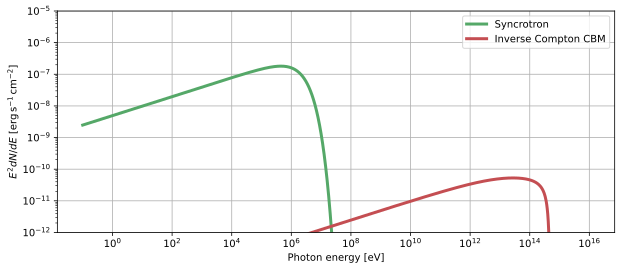
\includegraphics{chap3_files/figure-pdf/cell-3-output-1.pdf}

\subsubsection*{Measured muon flux}\label{measured-muon-flux}
\addcontentsline{toc}{subsubsection}{Measured muon flux}

In reality below 10 GeV muon decay and energy loss become important and
the Gaisser parametrization overestimates the muon flux as can be seen
in the plot below:

\begin{figure}[H]

{\centering \includegraphics[width=0.5\textwidth,height=\textheight]{images/atmmu.png}

}

\caption{Source: Particle Data Group}

\end{figure}%

As can be seen from the measured muon flux has the following
characteristics:

\begin{itemize}
\tightlist
\item
  Muons are the most numerous charged particles at sea level
\item
  The mean energy of muons at the ground is \(\sim\) 4 GeV.
\item
  The integral intensity of vertical muons above 1 GeV/c at sea level is
  \(\approx 70 \mathrm{m}^{-2} \mathrm{s}^{-1} \mathrm{sr}^{-1}\) or
  \(\approx 1 \mathrm{cm}^{-2} \mathrm{min}^{-1}\).
\end{itemize}

\subsection*{Muon Bundles}\label{muon-bundles}
\addcontentsline{toc}{subsection}{Muon Bundles}

Sometimes muons also come in groups or \textbf{bundles} of parallel
muons originated from the same primary CR. Muon bundles sometime look
like a single high energy muon. The multiplicity (number of muons in the
bundle) if can be measured is correlated with the mass of the orignal
CR. The image belowe shows a muon-bundle event observed with the MACRO
underground detector.

\includegraphics{images/macro-bundle.png}

\subsubsection*{Charge Ratio}\label{charge-ratio}
\addcontentsline{toc}{subsubsection}{Charge Ratio}

The muon charge ratio reflects the excess of \(\pi^+\) over \(\pi^-\)
and \(K^+\) over \(K^-\) and the fact that there are more protons than
neutrons in the primary spectrum.

\begin{figure}[H]

{\centering \includegraphics[width=0.5\textwidth,height=\textheight]{images/muon_ratio.png}

}

\caption{Source: Allkofer et. al.~Phys. Lett. B36, 425 (1971). Jokisch
et. al.~Phys. Rev.~D19, 1368 (1979)}

\end{figure}%

The increase with energy of the ratio is due to an increasing importance
of kaons coming from the process \$ p + N \rightarrow \Lambda +
K\^{}+\$.

Assuming the following reactions for the production of \(\pi^+\) and
\(\pi^{-}\):

\subsection*{Neutrinos Fluxes}\label{neutrinos-fluxes}
\addcontentsline{toc}{subsection}{Neutrinos Fluxes}

\begin{itemize}
\item
  Neutrinos are the most abundant CR product at sea level, yet they have
  only recently (compared to other particles) measured due to their
  extremely low cross-section.
\item
  The process giving neutrino fluxes are the same as for the muons (we
  saw already) plus the muon decay. Taking into account the decay of
  pions, kaons and muons gives to a flavor ratio of:
  \(\nu_\mu : \nu_e = 2:1\) and \(\nu_e/{\bar \nu_e} \sim \mu^+/\mu^-\)
\item
  At few GeV (\textgreater{} \(\epsilon_\mu\)) muons will not decay and
  \(\nu_e\) will be supressed as the main source of \(\nu_e\) is the
  muon decay.
\end{itemize}

\begin{Shaded}
\begin{Highlighting}[]
\ImportTok{from}\NormalTok{ daemonflux }\ImportTok{import}\NormalTok{ Flux}
\NormalTok{fl }\OperatorTok{=}\NormalTok{ Flux(location}\OperatorTok{=}\StringTok{\textquotesingle{}generic\textquotesingle{}}\NormalTok{, use\_calibration}\OperatorTok{=}\VariableTok{True}\NormalTok{, debug}\OperatorTok{=}\DecValTok{1}\NormalTok{)}
\NormalTok{egrid }\OperatorTok{=}\NormalTok{ np.logspace(}\DecValTok{0}\NormalTok{,}\DecValTok{5}\NormalTok{)}

\CommentTok{\# Start with a square Figure.}
\NormalTok{fig }\OperatorTok{=}\NormalTok{ plt.figure(figsize}\OperatorTok{=}\NormalTok{(}\DecValTok{6}\NormalTok{, }\DecValTok{6}\NormalTok{))}
\NormalTok{gs }\OperatorTok{=}\NormalTok{ fig.add\_gridspec(}\DecValTok{2}\NormalTok{, }\DecValTok{1}\NormalTok{, }
\NormalTok{                      left}\OperatorTok{=}\FloatTok{0.1}\NormalTok{, right}\OperatorTok{=}\FloatTok{0.9}\NormalTok{, bottom}\OperatorTok{=}\FloatTok{0.1}\NormalTok{, top}\OperatorTok{=}\FloatTok{0.9}\NormalTok{,}
\NormalTok{                      height\_ratios }\OperatorTok{=}\NormalTok{ (}\DecValTok{4}\NormalTok{, }\DecValTok{1}\NormalTok{), wspace}\OperatorTok{=}\FloatTok{0.05}\NormalTok{, hspace}\OperatorTok{=}\FloatTok{0.12}\NormalTok{)}
\CommentTok{\# Create the Axes.}
\NormalTok{ax\_1 }\OperatorTok{=}\NormalTok{ fig.add\_subplot(gs[}\DecValTok{0}\NormalTok{])}
\NormalTok{ax\_2 }\OperatorTok{=}\NormalTok{ fig.add\_subplot(gs[}\DecValTok{1}\NormalTok{], sharex}\OperatorTok{=}\NormalTok{ax)}

\NormalTok{ax\_1.plot(egrid, fl.flux(egrid, }\StringTok{"60"}\NormalTok{, }\StringTok{"numuflux"}\NormalTok{)}\OperatorTok{+}\NormalTok{fl.flux(egrid, }\StringTok{"60"}\NormalTok{, }\StringTok{"antinumu"}\NormalTok{), label}\OperatorTok{=}\VerbatimStringTok{r"$\textbackslash{}nu\_\{\textbackslash{}mu\}$ at $\textbackslash{}theta = 60\^{}\textbackslash{}circ$"}\NormalTok{)}
\NormalTok{ax\_1.plot(egrid, fl.flux(egrid, }\StringTok{"60"}\NormalTok{, }\StringTok{"nueflux"}\NormalTok{), label}\OperatorTok{=}\VerbatimStringTok{r"$\textbackslash{}nu\_}\SpecialCharTok{\{e\}}\VerbatimStringTok{$ at $\textbackslash{}theta = 60\^{}\textbackslash{}circ$"}\NormalTok{)}
\NormalTok{ax\_1.legend()}
\NormalTok{ax\_1.loglog()}
\NormalTok{ax\_1.grid()}
\NormalTok{ax\_2.plot(egrid, fl.flux(egrid, }\StringTok{"60"}\NormalTok{, }\StringTok{"numuflux"}\NormalTok{)}\OperatorTok{/}\NormalTok{fl.flux(egrid, }\StringTok{"60"}\NormalTok{, }\StringTok{"nueflux"}\NormalTok{), label}\OperatorTok{=}\VerbatimStringTok{r"\textbackslash{}nu\_\{\textbackslash{}mu\}"}\NormalTok{, lw}\OperatorTok{=}\DecValTok{2}\NormalTok{, color}\OperatorTok{=}\StringTok{"black"}\NormalTok{)}
\NormalTok{ax\_2.grid()}
\NormalTok{ax\_2.set\_xscale(}\StringTok{"log"}\NormalTok{)}
\NormalTok{ax\_2.set\_ylim(}\DecValTok{0}\NormalTok{, }\DecValTok{30}\NormalTok{)}
\NormalTok{ax\_2.set\_xlim(}\DecValTok{1}\NormalTok{, }\FloatTok{1e5}\NormalTok{)}
\NormalTok{ax\_1.set\_xlim(}\DecValTok{1}\NormalTok{, }\FloatTok{1e5}\NormalTok{)}
\NormalTok{ax\_2.set\_xlabel(}\VerbatimStringTok{r"$E\_\textbackslash{}nu$/GeV"}\NormalTok{)}
\NormalTok{ax\_1.set\_ylabel(}\VerbatimStringTok{r"$(E\_\textbackslash{}nu/\textbackslash{}mathrm\{ GeV\})\^{}3 \textbackslash{}Phi\_\textbackslash{}nu (\textbackslash{}mathrm\{ GeV\}\textbackslash{}mathrm\{ \textbackslash{};cm\}\^{}2\textbackslash{}mathrm\{ s\textbackslash{}; sr\})\^{}\{{-}1\}$"}\NormalTok{)}
\NormalTok{ax\_2.set\_ylabel(}\VerbatimStringTok{r"$\textbackslash{}Phi\_\{\textbackslash{}nu\_\textbackslash{}mu\} / \textbackslash{}Phi\_\{\textbackslash{}nu\_e\}$"}\NormalTok{)}
\end{Highlighting}
\end{Shaded}

\begin{verbatim}
Text(0, 0.5, '$\\Phi_{\\nu_\\mu} / \\Phi_{\\nu_e}$')
\end{verbatim}

\includegraphics{chap3_files/figure-pdf/cell-4-output-2.pdf}

\[ p + N \rightarrow p^\prime + N^\prime  + k \pi^+ + k \pi^- + r\pi^0 \]
\[ p + N \rightarrow n + N^\prime  + (k + 1) \pi^+ + k \pi^- + r\pi^0 \]

where \(k\) and \(r\) are the multiplicity of the particle species.
Assuming same cross sections we obtain:

\[ R = \frac{N(\pi^+)}{N(\pi^-)} = \frac{2k+1}{2k} = 1 + \frac{1}{2k} \]

for low energies \(k = 2\) and \(R \sim 1.25\)

\begin{tcolorbox}[enhanced jigsaw, colframe=quarto-callout-note-color-frame, opacitybacktitle=0.6, left=2mm, leftrule=.75mm, opacityback=0, colbacktitle=quarto-callout-note-color!10!white, breakable, bottomrule=.15mm, toprule=.15mm, colback=white, coltitle=black, bottomtitle=1mm, toptitle=1mm, titlerule=0mm, title=\textcolor{quarto-callout-note-color}{\faInfo}\hspace{0.5em}{Note}, arc=.35mm, rightrule=.15mm]

In astrophysical sources the ration 2:1 persists.
\hyperref[Charged_pion_decays]{Why pions don't decay in to electrons?}

\end{tcolorbox}

\subsection*{Fluxes and Kinematics}\label{fluxes-and-kinematics}
\addcontentsline{toc}{subsection}{Fluxes and Kinematics}

As mentioned neutrinos and muons are strongly correlated. However due
the two-body kinematics, the energy spectra of the \(\nu\)'s and
\(\mu\)'s from mesons decay are different. For example, the energy of
the muon in CoM is given by:

\[E_\mu^{*} = (m_\pi^2 + m_\mu^2)/2m_\pi = 109.8\;\mathrm{MeV}\]

and for the neutrino:

\[E_\nu^{*} = (m_\pi^2 - m_\mu^2)/2m_\pi = 29.8\;\mathrm{MeV}\]

In the laboratory system, the energies are boosted by the Lorentz factor
\(\gamma= E_\pi /m_\pi\), but as can be seen muon carry a much larger
fraction of energy than neutrinos. For energies about 1 TeV \$
\textless{} E\_\nu \textless{} 10\^{}3\$ TeV, the angle averaged
atmospheric \(\nu_\mu + {\bar \nu_\mu}\) can be approximated by a power
law spectrum:

\[\frac\mathrm{{d}N_{\nu_\mu + {\bar \nu_\mu}}}\mathrm{{d}E_\nu} = 7.8 \times 10^{-11}\left(\frac{E_\nu}{1\;\mathrm{TeV}}\right)^{-3.6} \mathrm{cm^2\;s^{-1}\;sr^{-1}\;GeV^{-1}}\]

\subsubsection*{Fluxes as Function of
Zenith}\label{fluxes-as-function-of-zenith}
\addcontentsline{toc}{subsubsection}{Fluxes as Function of Zenith}

Another difference with respect to the muon fluxes is their dependency
with respect to the zenith angle. Since atmospheric muons are not
absorved by the Earth, their spectrum spans to the whole sky. The
following plot shows the calculated neutrino flux at 1,300 m depth with
energies \(E_\nu = 10\) GeV.

\begin{figure}[H]

{\centering \includegraphics[width=0.4\textwidth,height=\textheight]{images/nu_zenith.png}

}

\caption{Source: \href{http://arxiv.org/abs/1210.5154}{arXiv:1210.5154}}

\end{figure}%

The peak at the horizon in the atmospheric neutrino flux is due to the
so-called \emph{secant theta effect}. This effect occurs because pions
and kaons that are produced nearly skimming the Earth have more flight
time in less dense atmosphere, so they have more chance to decay than
interact.

\subsection*{Prompt Fluxes}\label{prompt-fluxes}
\addcontentsline{toc}{subsection}{Prompt Fluxes}

Apart from kaons and pions, charmed messons will also be produced in the
atmosphere. Charm particles have lifetimes so short (\(10^{-12}\)s) they
almost alway decay before interacting. Muons and neutrinos from charm
decay are called \emph{prompt} muons/neutrinos. They have the following
peculiarities:

\begin{itemize}
\tightlist
\item
  The energy spectrum follows the one of the primary cosmic rays ie that
  of \(\sim E^{-2.7}\).
\item
  Since there is no competition between decay and interaction of the
  charm particle, the \emph{prompt} flux is fully \textbf{isotropic}.
\item
  Since neutrinos are produced in 3-body decays they produced the same
  amount of \(\nu_\mu\) and \(\nu_e\).
\end{itemize}

It is important to note that the prompt fluxes have not been observed
yet.

\section*{Particles Underground}\label{particles-underground}
\addcontentsline{toc}{section}{Particles Underground}

\markright{Particles Underground}

\subsection*{Muon Interactions}\label{muon-interactions}
\addcontentsline{toc}{subsection}{Muon Interactions}

When muon reaches the ground the will experience the following
interactions when travelling through matter with a higher density than
air. The will losse energy mostly through the following processes:

\begin{itemize}
\tightlist
\item
  \textbf{Ionization.} The continuous energy loss of muons passing
  through a medium as it ionize the material along the path. We saw
  however that ionization is mostly independent of the material, as most
  of them have values of \(Z/A \sim 0.5\).
\end{itemize}

\includegraphics[width=0.3\textwidth,height=\textheight]{index_files/mediabag/images/muon_ionization.pdf}

\begin{itemize}
\tightlist
\item
  \textbf{Bremsstrahlung.} Also called braking radiation. In the
  electric field of a nucleus or atomic electrons, muons can radiate
  high energy photons. If the photon has energy enough it can initiate
  an electromagnetic shower.
\end{itemize}

\includegraphics[width=0.3\textwidth,height=\textheight]{index_files/mediabag/images/muon_bremsstrahlung.pdf}

\begin{itemize}
\tightlist
\item
  \textbf{Pair production.} A muon can radiate a virtual photon which,
  again in the electric field of a nucleus, can convert into a real
  \(e^+e^-\) pair. As in the case of bremsstrahlung, the pair production
  will initate an electromagnetic shower.
\end{itemize}

\includegraphics[width=0.3\textwidth,height=\textheight]{index_files/mediabag/images/muon_pair-production.pdf}

\begin{itemize}
\tightlist
\item
  \textbf{Photonuclear interactions.} A muon can radiate a virtual
  photon which directly interacts with a nucleus in the muon propagation
  medium. The interaction is either electromagnetic or following the
  fluctuation of the photon into a quark-antiquark pair (i.e.~a virtual
  vector meson). This interaction will generate an hadronic shower.
\end{itemize}

\includegraphics[width=0.3\textwidth,height=\textheight]{index_files/mediabag/images/muon_photonuclear.pdf}

\subsection*{Muon Energy losses}\label{muon-energy-losses}
\addcontentsline{toc}{subsection}{Muon Energy losses}

The energy losses due to ionization are continuous while in radiation
processes the energy is lost in bursts along the muon path. When a muon
is travelling through a dielectric medium like ice or water, it will
emit cherenkov photons as wells, but due to the stochastics energy
losses electromagnetic and hadronic showers are generated along the muon
track. The following figure illustrates this process:

\includegraphics[width=0.8\textwidth,height=\textheight]{index_files/mediabag/images/muon_energylosses.pdf}

It is worth noting that photonuclear interactions are subdominant when
compared to bremsstrahlung and pair-production, so most of the showers
will be electromagnetic showers. The equation that describes the energy
loss for muons at high energy can be simplified to:

\[\frac{\mathrm{ d}E_\mu}{\mathrm{ d}X} = -\alpha -\beta E_\mu\]

where \(X\) is the thickness of the material (in \(\mathrm{ g/cm}^2\)),
\(\alpha\) is the energy loss due to ionization and
\(\beta = \beta_{br} + \beta_{pair} + \beta_{ph}\) are the three
discrete energy loss processes: bremsstrahlung, electron-positron
production and electromagnetic interaction with the nuclei. Thickness is
also given sometimes in units of meters water equivalent (1 m.w.e. =
\(10^2 \mathrm{\; g/cm^2}\)). Due to the energy dependency of the
radiative processes, higher energy muons will have more stochastic
energy losses than lower energy muons.

The \textbf{critical energy} is when both losses are equal, ie
\(\epsilon_\mu = \alpha/\beta\). Typical values are
\(\alpha \simeq 2 \mathrm{ \;MeV\;g}^{-1} \mathrm{ \;cm}^2\) and
\(\beta \simeq 4 \times 10^{-6} \;\mathrm{ g^{-1}\;cm^2}\), so
\(\epsilon_\mu \approx 500\) GeV.

The following plots showd simulated muons bundles in IceCube. The
stochastic energy losses are particular clear in the right figure.

\includegraphics{images/musmooth.jpg}
\includegraphics{images/mustochastic.jpg}

\subsection*{Muon Range}\label{muon-range}
\addcontentsline{toc}{subsection}{Muon Range}

By solving the energy loss equation we can estimate the range \(R\) for
a muon \(E_\mu\), ie the underground depth this muon will reach until
its energy is 0 (in reality the muon when reaching low energies will
decay) (see Exercises 2):

\[ R(E_\mu) = \frac{1}{\beta}\log\left( 1 + \frac{E_\mu}{\epsilon_\mu}\right)\]

Assuming the muon spectrum at sea level can be approximated to a power
law \(I_\mu(>E_\mu) = AE_\mu^{-\gamma}\) and using the relationship
between range and energy we can write the \emph{depth-intensity
relation} (DIR):

\[I_\mu(>E_\mu, R) = A\left[\frac{\alpha}{\beta}(e^{\beta R} - 1)\right]^{-\gamma}\]

The plot below shows the depth-intensity muons for vertical directions.
The grey-area are neutrino-induced muons (horizontal, up-wards)

\includegraphics{images/muon-depth.png}

\subsection*{Neutrino Interactions}\label{neutrino-interactions}
\addcontentsline{toc}{subsection}{Neutrino Interactions}

\subsubsection*{Weak interaction}\label{weak-interaction}
\addcontentsline{toc}{subsubsection}{Weak interaction}

Neutrinos feel only the weak force thus interactions with matter
mediated by W and Z bosons with cross-sections typical of weak
processes. Feynman diagrams factor along two lines:

\begin{itemize}
\tightlist
\item
  Neutral current (NC) interactions - exchange of Z
\item
  Charged current (CC) interaction - exchange of W\(^{\pm}\)
\end{itemize}

\includegraphics{index_files/mediabag/images/neutrino-interactions.pdf}

Neutrinos will scatter from electrons as well as nuclear matter.

\begin{itemize}
\item
  For energies \(E_\nu < 1\) GeV neutrinos interact with hadronds via
  \textbf{elastic} or \textbf{quasielastic scattering}.
\item
  For energies \(E_\nu \gg 1\) GeV neutrinos do not scatter on hadronds
  as a compound of quarks, they start to \emph{see} and interact
  directly the quarks, \textbf{Deep Inelastic Scattering}.
\end{itemize}

\subsection*{Neutrino cross-sections at GeV
energies}\label{neutrino-cross-sections-at-gev-energies}
\addcontentsline{toc}{subsection}{Neutrino cross-sections at GeV
energies}

The anti-neutrino cross-section at GeV energies is a factor
\textasciitilde2 lower (naively should be 3, but the factor 2 comes from
the structure function of the nucleus) than the neutrino cross-section
due to the helicity.

\includegraphics{images/pdg_plot.gif}

At \(E_\nu \gg 1\) GeV the total DIS cross-section (ie, assuming CC and
NC together) can be approximated to:

\[\sigma_{\nu p} \simeq 0.69 \times 10^{-38} \left(\frac{E_\nu}{ 1 \rm{\; GeV}}\right) \rm{ \; cm}^2\]
\[\sigma_{\bar{\nu} p} \simeq 0.35 \times 10^{-38}\left(\frac{E_\nu}{ 1 \rm{\; GeV}}\right) \rm{ \; cm}^2\]

Sometimes the cross-section is expressed as \(\nu + N\) where \(N\) is
the nucleon definition as:

\[N = \frac{n+p}{2}\]

Earth is transparent to GeV neutrinos

We are going to calculate the mean free path of neutrinos of energies of
\(\sim GeV\). Note that mean free path can be expressed as:

\[l = \frac{1}{n_N \sigma_{\nu N}}\]

where \(n_N\) is the number density of \emph{nucleons} and not atoms. As
we saw in lecture 2 we can re-express the number density as:

\[n_N = \frac{N_A}{\mathcal{M}}\rho\]

where \(\mathcal{M}\) is the molar mass of one mole of nucleons and
\(\rho\) is the mass density of the medium. However, by definition a mol
of nucleons has a mass of 1 g (Remember that a mol of \(^{12}C\) atoms
has a mass of 12 g). So, we can rewrite as \(n_N = N_A \rho\). Below
there is another way to estimate the mean free path:

\begin{Shaded}
\begin{Highlighting}[]
\ImportTok{from}\NormalTok{ astropy }\ImportTok{import}\NormalTok{ constants }\ImportTok{as}\NormalTok{ ct}
\ImportTok{from}\NormalTok{ astropy }\ImportTok{import}\NormalTok{ units }\ImportTok{as}\NormalTok{ u}
\CommentTok{\#Earth mass}
\BuiltInTok{print}\NormalTok{ (ct.M\_earth)}

\CommentTok{\#Neutron/proton mass}
\BuiltInTok{print}\NormalTok{ (ct.m\_n)}

\CommentTok{\#Earth radius}
\BuiltInTok{print}\NormalTok{ (ct.R\_earth)}

\CommentTok{\#number of nucleons}
\NormalTok{N }\OperatorTok{=}\NormalTok{ ct.M\_earth}\OperatorTok{/}\NormalTok{ct.m\_n }

\CommentTok{\#Earth volume}
\NormalTok{Ve }\OperatorTok{=} \DecValTok{4}\OperatorTok{/}\DecValTok{3}\OperatorTok{*}\NormalTok{np.pi}\OperatorTok{*}\NormalTok{ct.R\_earth}\OperatorTok{**}\DecValTok{3}

\CommentTok{\#Nucleon density}
\NormalTok{Nd }\OperatorTok{=}\NormalTok{ N}\OperatorTok{/}\NormalTok{Ve}

\CommentTok{\#Cross section}
\NormalTok{s }\OperatorTok{=} \FloatTok{1e{-}38} \OperatorTok{*}\NormalTok{ u.cm}\OperatorTok{**}\DecValTok{2}
\CommentTok{\#Mean free path:}
\NormalTok{L }\OperatorTok{=} \DecValTok{1}\OperatorTok{/}\NormalTok{(s }\OperatorTok{*}\NormalTok{ Nd.to(}\DecValTok{1}\OperatorTok{/}\NormalTok{u.cm}\OperatorTok{**}\DecValTok{3}\NormalTok{))}

\BuiltInTok{print}\NormalTok{ (}\SpecialStringTok{f"The mean free path is: }\SpecialCharTok{\{}\NormalTok{L}\SpecialCharTok{.}\NormalTok{to(u.km)}\SpecialCharTok{\}}\SpecialStringTok{"}\NormalTok{)}
\end{Highlighting}
\end{Shaded}

\begin{verbatim}
  Name   = Earth mass
  Value  = 5.972167867791379e+24
  Uncertainty  = 1.3422009501651213e+20
  Unit  = kg
  Reference = IAU 2015 Resolution B 3 + CODATA 2018
  Name   = Neutron mass
  Value  = 1.67492749804e-27
  Uncertainty  = 9.5e-37
  Unit  = kg
  Reference = CODATA 2018
  Name   = Nominal Earth equatorial radius
  Value  = 6378100.0
  Uncertainty  = 0.0
  Unit  = m
  Reference = IAU 2015 Resolution B 3
The mean free path is: 304808158.9154454 km
\end{verbatim}

\subsection*{Neutrino cross-sections at TeV
energies}\label{neutrino-cross-sections-at-tev-energies}
\addcontentsline{toc}{subsection}{Neutrino cross-sections at TeV
energies}

\begin{itemize}
\item
  At low energies the valence quark parton distribution dominates and
  both the neutrino NC and CC cross-section grows linear with energy
  since the transfer momemtum \(q^2 \ll M_{W,Z}\) and so the propagator
  term is \(\sim 1/M^2_{W,Z}\)
\item
  Above 10\(^{4}\) GeV where the gauge-boson propagator restricts the
  momentum transfer to values near \(M_{W,Z}\)
  (\(\sim 1/(q^2 - M^2_{W,Z})\)) and damps the cross-section increase.
\end{itemize}

\includegraphics{images/break_cc_new.png}

\subsection*{High energy
Cross-Sections}\label{high-energy-cross-sections}
\addcontentsline{toc}{subsection}{High energy Cross-Sections}

The following shows the neutrino cross section:

\begin{figure}[H]

{\centering \includegraphics{images/uhenucx.png}

}

\caption{Calculated neutrino cross sections taken from
\href{http://arxiv.org/abs/1309.1764}{arXiv:1309.1764}}

\end{figure}%

\begin{itemize}
\item
  At high energies the asymetry between neutrinos and antineutrinos is
  lost due to the interaction with \emph{sea quarks} (\(q\bar{q}\))
\item
  Neutrinos interact mostly with hadrons (quarks) instead of electrons
  due the their larger target mass. However at \(E_\nu \approx 6.3\) PeV
  the Glashow resonance appears: \({\hbar \nu_e} + e \rightarrow W\)
  making the cross-section higher than the one with hadrons. \#\#\#
  Earth Opaque to PeV Neutrinos
\item
  At about 100 TeV the mean free path for neutrino-nucleus scattering is
  about 10\(^{10}\) c.m.w.e. which is about the matter thickness along
  the Earth diameter.
\item
  This means that UHE neutrino observatories (like IceCube) the flux of
  neutrinos comming from the nadir is stronly suppressed.
\item
  There is only one exception. A very high energy beam of \(\nu_\tau\)
  at one side of the Earth \(E\gg 1\) PeV can end up at the other side
  as lower energy \(\nu_\tau, \nu_e,\nu_\mu\) thought the \textbf{tau
  regeneration} effect:
  \(\nu_\tau \rightarrow \tau \rightarrow \nu_\tau\)
\end{itemize}

\subsection*{Neutrino signatures in a
detector}\label{neutrino-signatures-in-a-detector}
\addcontentsline{toc}{subsection}{Neutrino signatures in a detector}

\includegraphics{images/nu_signatures.png}

\begin{itemize}
\tightlist
\item
  \begin{enumerate}
  \def\labelenumi{\alph{enumi})}
  \setcounter{enumi}{1}
  \tightlist
  \item
    In CC \(\nu_e\) interactions an hadronic and EM shower initiated by
    the \(e\) is produced. About 20\% of the energy goes in the hadronic
    shower and 80\% to the lepton and therfore to the EM shower.
  \end{enumerate}
\item
  \begin{enumerate}
  \def\labelenumi{\alph{enumi})}
  \setcounter{enumi}{3}
  \tightlist
  \item
    In CC \(\nu_\tau\) d) interaction again an hadronic and EM shower
    are produced as the \(\tau\) decays almost inmediately to pions or
    other charge leptons. In the decay another \(\nu_\tau\) is produced
    \textbf{tau regeneration effect}. At very high energyes the two
    showers can be separated giving a \emph{double bang} signature or a
    \emph{lollipop} if the first shower happens outside the detector.
  \end{enumerate}
\item
  \begin{enumerate}
  \def\labelenumi{\alph{enumi})}
  \setcounter{enumi}{2}
  \tightlist
  \item
    In CC \(\nu_\mu\) the muon only undergoes radiation losses (not
    ionization) and hence the track of the muon can be reconstructed.
  \end{enumerate}
\item
  \begin{enumerate}
  \def\labelenumi{\alph{enumi})}
  \tightlist
  \item
    In NC only an hadronic shower is visible.
  \end{enumerate}
\end{itemize}

\subsection*{Event rate in an underground
experiment.}\label{event-rate-in-an-underground-experiment.}
\addcontentsline{toc}{subsection}{Event rate in an underground
experiment.}

An estimate of the detection rate of neutrino events is equivalent to
calculate the rate of a neutrino-induced muon/cascades flux:

\[R(E_{vis}, \theta) = \int_{E_{vis}} P_{\nu\rightarrow l} (E_\nu, E_{vis}) P_{shadow}(\theta, E_\nu) \frac{\mathrm{ d}N_\nu}{\mathrm{ d}E_\nu}\mathrm{ d}E_\nu\]

where * \(P_{\nu\rightarrow l}(E_\nu, E_{vis})\). Probability that a
neutrino interacts with an nucleus to produce a \(\mu\) or an EM or
hadronic cascade with a minimum energy \(E_{vis}\) \emph{visible} in the
detector. * \(P_{shadow} (\theta, E_\nu)\). Probability of neutrino with
zenith angle \(\theta\) and energy \(E_\nu\) of being absorved by Earth.
* \({\mathrm{ d}N_\nu}/{\mathrm{ d}E_\nu}\). Neutrino flux at the
surface.

\subsection*{\texorpdfstring{Interaction probability:
\(P_{\nu\rightarrow l}\)}{Interaction probability: P\_\{\textbackslash nu\textbackslash rightarrow l\}}}\label{interaction-probability-p_nurightarrow-l}
\addcontentsline{toc}{subsection}{Interaction probability:
\(P_{\nu\rightarrow l}\)}

The probability of a neutrino to produce a lepton or shower visible in
the detector can be writen as:

\[P_{\nu \rightarrow l} = N_A \int_{E_{min}}^{E_\nu} \mathrm{ d}E_l \frac{\mathrm{ d}\sigma}{\mathrm{ d}E_l}r_l(E_l, E_{vis})\]

where \(r_l\) is the detection range of the produced lepton/cascade with
energy \(E_l\) ending with the minimal energy \(E_{vis}\), and
\({\mathrm{ d}\sigma}/{\mathrm{ d}E_l}\) is the neutrino cross-section
to produce a lepton/cascade with energy \(E_l\).

At high energy the event rate is dominated by neutrino-induced muons due
to the long range of the high energy muons.

\subsection*{\texorpdfstring{Earth Shadow:
\(P_{shadow}\)}{Earth Shadow: P\_\{shadow\}}}\label{earth-shadow-p_shadow}
\addcontentsline{toc}{subsection}{Earth Shadow: \(P_{shadow}\)}

The mean free path of neutrinos can be expressed as
\(\lambda = (N_A \sigma_{tot})^{-1}\). The shadow fact then can be
expressed as:

\[P_{shadow} = e^{-N_A \sigma_{tot} X(\theta)}\]

Where \(X(\theta)\) is the column depth travelled by the neutrino
through the Earth with a zenith angle \(\theta\).

See \textbf{Exercises 2} for an evaluation of the event rate in an
underground detector.

\subsection*{Neutrino Oscillations}\label{neutrino-oscillations}
\addcontentsline{toc}{subsection}{Neutrino Oscillations}

Neutrinos are generated in flavor eingenstate however propagation is
done in mass eingenstate, since each planar wave has a different
frecuency given their different masses, the neutrino detected (also in
flavor eingenstate) will have a different interference pattern than the
one generated given rise to neutrino flavor oscillations.

\begin{itemize}
\item
  As a result of these changes in relative phases, neutrinos oscillate
  from one flavor to another as they travel. Low-energy neutrinos
  oscillate in a shorter distance than high-energy neutrinos.
\item
  A curious aspect of quantum physics is that only the
  \textbf{probability of the flavor of neutrino changes as it travels}.
\item
  The neutrino \emph{only becomes a definite flavor when it interacts}
  in a detector - by finding whether an electron, muon, tau is created.
\end{itemize}

\subsection*{The PMNS Matrix}\label{the-pmns-matrix}
\addcontentsline{toc}{subsection}{The PMNS Matrix}

The Pontecorvo-Maki-Nakagawa-Sakata matrix is the one that relates the
mass eingenstates with the flavor eingenstates:

\[\begin{pmatrix} \nu_e \\ \nu_\mu \\ \nu_\tau \end{pmatrix} = U_{PMNS} \begin{pmatrix} \nu_1 \\ \nu_2 \\ \nu_1 \end{pmatrix}\]

with:

\[
\begin{aligned}
U_{PMNS} &= 
\begin{pmatrix} 
c_{12}c_{13} & s_{12}c_{13} & s_{13}e^{-i\delta} \\
-s_{12}c_{23} - c_{12}s_{23}s_{13}e^{i\delta} & c_{12}c_{23} - s_{12}s_{23}s_{13}e^{i\delta} & s_{23}c_{13} \\
s_{12}s_{23} - c_{12}c_{23}s_{13}e^{i\delta} & -c_{12}s_{23} - s_{12}c_{23}s_{13}e^{i\delta} & c_{23}c_{13} \end{pmatrix} \\
&= \begin{pmatrix} 
1 & 0 & 0 \\ 0 & c_{23} & s_{23} \\ 0 & -s_{23} & c_{23} 
\end{pmatrix}
\begin{pmatrix} 
c_{13} & 0 & s_{13}e^{-i\delta} \\ 0 & 1 & 0 \\ -s_{13}e^{i\delta} & 0 & c_{13} 
\end{pmatrix}
\begin{pmatrix} 
c_{12} & s_{12} & 0 \\ -s_{12} & c_{12} & 0 \\ 0 & 0 & 1 
\end{pmatrix}
\end{aligned}
\]

where \(s_{ij} = \sin \theta_{ij}\), \(c_{ij} = \cos \theta_{ij}\). The
term \(\delta\) is a CP violation term, if \(s_{13} = 0\) we won't be
able to measure \(\delta\) as it always multiplies \(s_{13}\)

\subsection*{The 2-flavor mixing case}\label{the-2-flavor-mixing-case}
\addcontentsline{toc}{subsection}{The 2-flavor mixing case}

Let's assume 2 flavor eigenstates identified as rotations of 2 mass
eigenstates:

\[\begin{pmatrix} \nu_e \\ \nu_\mu \end{pmatrix} = \begin{pmatrix} \cos\theta & \sin\theta \\ -\sin\theta & \cos\theta \end{pmatrix} \begin{pmatrix} \nu_1 \\ \nu_2 \end{pmatrix}.\]

The angle \(\theta\) is called the mixing angle.

The mass eigenstates evolve as plane waves with fixed momemtum \(p\):

\[|\nu_{i}(t, x)\rangle = e^{ -i (E_{i} t - p_i x) }|\nu_{i}(0,0)\rangle\]

Let's imagine we start at \((x,t) = (0,0)\) with a pure beam of
\(\nu_e\):

\[\begin{pmatrix} 1 \\ 0 \end{pmatrix} = \begin{pmatrix} \cos\theta & \sin\theta \\ -\sin\theta & \cos\theta \end{pmatrix} \begin{pmatrix} \nu_1(0,0) \\ \nu_2(0,0) \end{pmatrix}.\]

\[|\nu_{1}(0,0)\rangle = \cos \theta\]
\[|\nu_{2}(0,0)\rangle = \sin \theta\]

and as they evolved:

\[|\nu_{1}(t,x)\rangle = \cos \theta e^{ -i (E_{1} t - p_1 x)  }\]
\[|\nu_{2}(t,x)\rangle = \sin \theta e^{ -i (E_{2} t - p_2 x) }\]

So after a while the wave form of the \(\nu_\alpha\) is given by:

\[|\nu_{e}(t, x)\rangle = \cos^2 \theta e^{ -i (E_{1} t - p_1 x)  } + \sin^2 \theta e^{ -i (E_{2} t - p_2 x) } = A_e\]
\[|\nu_{\mu}(t, x)\rangle = -sin\theta\cos \theta e^{ -i (E_{1} t - p_1 x)  } + \cos\theta\sin \theta e^{ -i (E_{2} t - p_2 x) } = A_e\]

\subsubsection*{Example of survival probability for the 2-flavor
mixing}\label{example-of-survival-probability-for-the-2-flavor-mixing}
\addcontentsline{toc}{subsubsection}{Example of survival probability for
the 2-flavor mixing}

\[\begin{aligned}
P(\nu_e \rightarrow \nu_\mu) = \left|\langle \nu_{\mu}(t,x)|\nu_{e}(0,0)\rangle\right|^2 &=\left|\cos\theta \sin\theta (e^{i(E_2 t - p_2 x)} - e^{i(E_1 t -p_1 x)})\right|^2\\
&=
\cos^2\theta\sin^2\theta \left|e^{i(E_2 t - p_2 x)} - e^{i(E_1 t -p_1 x)}\right|^2
\end{aligned}
\]

using \(e^{\pm ix} = \cos x \pm i\sin x\)

\[
\begin{aligned}
P(\nu_e \rightarrow \nu_\mu)&= 2 \cos^2\theta\sin^2\theta ( 1 - \cos (E_2t - p_2x - E_1 t - p_1 x))\\
&= \sin^2 2\theta \sin^2 \left(\frac{(E_2 - E_1)t - (p_2 - p_1)x }{2}\right) \\ 
&=\sin^2 2\theta \sin^2 \left(\frac{\Delta m_{12}^2 L}{4E}\right)
\end{aligned}
\]

using \(p_i = \sqrt{E^2_i -m_i^2}\sim E_i(1-\frac{m^2_i}{E_i^2})\), and
in natural units \(t = x = L\) we can write the phase difference as:

\[(E_2 - E_1)t - (p_2 - p_1)x = (\frac{m_1^2}{2E_1}-\frac{m_2^2}{2E_2})L = \frac{\Delta m_{12}^2L}{2E}\]

And the survival probability is:

\[P(\nu_e \rightarrow \nu_e)  = 1 - P(\nu_e \rightarrow \nu_\mu) = 1- \sin^2 2\theta \sin^2\left(\frac{\Delta m_{12}^2 L}{4E}\right)\]

Replacing \(\hbar\) and \(c\) the expression can be written as:

\[P(\nu_e \rightarrow \nu_e)  = 1 - \sin^2 2\theta \sin^2\left[1.27 \left(\frac{\Delta m^2_{12}}\mathrm{{ eV}^2}\right)\frac{L/\rm{ km}}{E/\rm{ GeV}}\right]\]

We assumed that the mass eigenstates are created with the same energy or
momentum and so \(E_i = E_j\).This assumption is not necessary and it
comes from the fact we use the plane wave approximation. Using the
correct formalism of wave packets the result is the same.

\subsection*{\texorpdfstring{Tutorial III: Plot the survival probability
of
\(\nu_e \rightarrow \nu_e\)}{Tutorial III: Plot the survival probability of \textbackslash nu\_e \textbackslash rightarrow \textbackslash nu\_e}}\label{tutorial-iii-plot-the-survival-probability-of-nu_e-rightarrow-nu_e}
\addcontentsline{toc}{subsection}{Tutorial III: Plot the survival
probability of \(\nu_e \rightarrow \nu_e\)}

\begin{Shaded}
\begin{Highlighting}[]
\ImportTok{import}\NormalTok{ astropy.units }\ImportTok{as}\NormalTok{ u}

\NormalTok{L }\OperatorTok{=} \DecValTok{180} \CommentTok{\# km}

\NormalTok{delta\_m\_sun }\OperatorTok{=} \FloatTok{7.0e{-}5} \CommentTok{\# eV\^{}2}
\NormalTok{sin\_square\_theta\_12 }\OperatorTok{=} \FloatTok{0.84} \CommentTok{\#maximum mixing}


\KeywordTok{def}\NormalTok{ prob\_survival(E, L):}
    \ControlFlowTok{return} \DecValTok{1} \OperatorTok{{-}}\NormalTok{ sin\_square\_theta\_12 }\OperatorTok{*}\NormalTok{ np.sin(}\FloatTok{1.27}\OperatorTok{*}\NormalTok{delta\_m\_sun }\OperatorTok{*}\NormalTok{ L }\OperatorTok{/}\NormalTok{ E)}\OperatorTok{**}\DecValTok{2}

\NormalTok{fig, ax }\OperatorTok{=}\NormalTok{ plt.subplots(figsize}\OperatorTok{=}\NormalTok{(}\DecValTok{10}\NormalTok{,}\DecValTok{4}\NormalTok{))}
\NormalTok{ax.set\_ylim(}\DecValTok{0}\NormalTok{,}\DecValTok{1}\NormalTok{)}
\NormalTok{ax.set\_xlabel(}\VerbatimStringTok{r"$E\_\textbackslash{}nu (\textbackslash{}mathrm\{ MeV\})$"}\NormalTok{)}
\NormalTok{ax.set\_ylabel(}\StringTok{"$P\_}\SpecialCharTok{\{ee\}}\StringTok{$"}\NormalTok{)}

\NormalTok{E }\OperatorTok{=}\NormalTok{ np.linspace(}\FloatTok{0.1}\NormalTok{, }\DecValTok{15}\NormalTok{, }\DecValTok{1000}\NormalTok{) }\CommentTok{\#in MeV}

\NormalTok{ax.plot(E, prob\_survival(E}\OperatorTok{*}\FloatTok{1e{-}3}\NormalTok{,L), lw}\OperatorTok{=}\DecValTok{2}\NormalTok{, }
\NormalTok{        label}\OperatorTok{=}\StringTok{"L = }\SpecialCharTok{\%i}\StringTok{ km}\CharTok{\textbackslash{}n}\StringTok{"}\OperatorTok{\%}\NormalTok{L}\OperatorTok{+}\VerbatimStringTok{r"$P\_}\SpecialCharTok{\{ee\}}\VerbatimStringTok{ = 1 {-}\textbackslash{}sin\^{}2 2\textbackslash{}theta\textbackslash{}sin\^{}2(\textbackslash{}Delta m\^{}2L/4E\_\textbackslash{}nu)$"}\NormalTok{)}
\NormalTok{plt.legend(loc}\OperatorTok{=}\StringTok{"best"}\NormalTok{)}
\NormalTok{ax.grid()}
\NormalTok{plt.show()}
\end{Highlighting}
\end{Shaded}

\includegraphics{chap3_files/figure-pdf/cell-6-output-1.pdf}

Eventually at low enough E / long baselines, neutrino beam becomes fully
mixed and energy resolution and source extent conspire to produce 50/50
beam.

\begin{Shaded}
\begin{Highlighting}[]
\NormalTok{y, x }\OperatorTok{=}\NormalTok{ np.meshgrid(np.linspace(}\DecValTok{50}\NormalTok{,}\DecValTok{180}\NormalTok{,}\DecValTok{100}\NormalTok{), np.linspace(}\FloatTok{0.1}\NormalTok{, }\DecValTok{15}\NormalTok{, }\DecValTok{100}\NormalTok{) )}
\NormalTok{z }\OperatorTok{=}\NormalTok{ prob\_survival(x}\OperatorTok{*}\FloatTok{1e{-}3}\NormalTok{,y)}
\NormalTok{fig }\OperatorTok{=}\NormalTok{ plt.figure(figsize}\OperatorTok{=}\NormalTok{(}\DecValTok{10}\NormalTok{,}\DecValTok{5}\NormalTok{))}
\NormalTok{ax }\OperatorTok{=}\NormalTok{ plt.subplot(}\DecValTok{111}\NormalTok{)}
\NormalTok{img }\OperatorTok{=}\NormalTok{ ax.pcolormesh(x, y, z, cmap }\OperatorTok{=} \StringTok{\textquotesingle{}RdBu\textquotesingle{}}\NormalTok{, shading}\OperatorTok{=}\StringTok{\textquotesingle{}auto\textquotesingle{}}\NormalTok{)}

\NormalTok{cax }\OperatorTok{=}\NormalTok{ fig.colorbar(img)}
\NormalTok{ax.set\_ylabel(}\StringTok{"Distance (km)"}\NormalTok{)}
\NormalTok{ax.set\_xlabel(}\VerbatimStringTok{r"$E\_\textbackslash{}nu (\textbackslash{}mathrm\{ MeV\})$"}\NormalTok{)}
\NormalTok{cax.set\_label(}\StringTok{"Probability"}\NormalTok{)}
\end{Highlighting}
\end{Shaded}

\includegraphics{chap3_files/figure-pdf/cell-7-output-1.pdf}

\subsection*{General case}\label{general-case}
\addcontentsline{toc}{subsection}{General case}

Taking greek letters of the flavor eingenstates and latin letter the
mass eingenstates we can write:

\[|\nu_\alpha(x,t)\rangle = \sum_{k=1,2,3} U_{\alpha k} |\nu_k (x,t)\rangle = \sum_{k=1,2,3} U_{\alpha k} e^{-i\Phi_k}|\nu_k (0,0)\rangle\]

inverting the mixing matrix we have:

\[|\nu_k (0,0)\rangle =\sum_\gamma U^*_{\gamma  k} |\nu_\gamma(0,0)\rangle\]

putting it in the equation above:

\[|\nu_\alpha(x,t)\rangle =\sum_{k=1,2,3} U_{\alpha k} e^{-i\Phi_k}\sum_\gamma U^*_{\gamma  k} |\nu_\gamma(0,0)\rangle\]

If we want to evaluate the probability of finding a neutrino \(\beta\)
when we had \(\alpha\) is the transition amplitude is given by:

\[\begin{aligned}
\mathcal{A}(\nu_\alpha(0,0)\rightarrow \nu_\beta(x,t)) &= \langle \nu_\beta(x,t)|\nu_\alpha(0,0)\rangle \\
&= \sum_\gamma \sum_k U_{\gamma k}e^{i\Phi_k}U^*_{\beta k}\langle \nu_\gamma(0,0)|\nu_\alpha(0,0)\rangle \\
&= \sum_k U_{\alpha  k}e^{i\Phi_k}U^*_{\beta k}
\end{aligned}\]

where we used the fact that flavor eingenstates are ortogonal and hence
\(\langle \nu_\gamma(0,0)|\nu_\alpha(0,0)\rangle = \delta_{\gamma,\alpha}\).

The oscillation probability is then:

\[\begin{aligned}
P(\nu_\alpha \rightarrow \nu_\beta) = |\mathcal{A}(\nu_\alpha(0,0)\rightarrow \nu_\beta(x,t))|^2 &= \left|\sum_k U_{\alpha i}e^{i\Phi_i}U^*_{\beta i}\right|^2\\
&=\sum_i U_{\alpha i}e^{i\Phi_i}U^*_{\beta i}\sum_j U^*_{\alpha j}e^{-i\Phi_j}U_{\beta j}\\
&=\sum_j\sum_i U_{\alpha i}U^*_{\beta i}U^*_{\alpha j}U_{\beta j}e^{-i(\Phi_j-\Phi_i)}
\end{aligned}\]

where \(\Phi_i = E_i t- p_i x\) and so:

\[\Phi_i - \Phi_j = (E_i - E_j)t - (p_i -p_j)x\]

using \(p_i = \sqrt{E^2_i -m_i^2}\sim E_i(1-\frac{m^2_i}{E_i^2})\) we
can write the phase difference as:

\[\Phi_i - \Phi_j = (\frac{m_i^2}{2E_i}-\frac{m_j^2}{2E_j})L = \frac{\Delta m_{ij}^2L}{2E}\]

where we used the fact that at relativistic speeds \(t = x = L\) and a
dodgy approximation where we assumed that the mass eigenstates are
created with the same energy or momentum and so \(E_i = E_j\).This
assumption is not necessary, but we find that whatever assumption is
made you get the the same result. The fact that we have to make such an
approximation comes from the way that we are modelling the mass
eigenstates as plane waves. If we were to do the analysis assuming that
the mass states were wavepackets instead we would not need the equal
momentum (equal energy) assumption and would still get the same answer.

With this we can rewrite the oscillation probability as:

\[\begin{matrix}P(\nu_\alpha \rightarrow \nu_\beta)=\delta_{\alpha\beta} & - & 4{\displaystyle \sum_{i>j}\mathrm{ Re}(U_{\alpha i}^{*}U_{\beta i}U_{\alpha j}U_{\beta j}^{*}})\sin^{2}(\frac{\Delta m_{ij}^{2}L}{4E})\\ & + & {\displaystyle 2\sum_{i>j}\mathrm{ Im}(U_{\alpha i}^{*}U_{\beta i}U_{\alpha j}U_{\beta j}^{*})\sin(}\frac{\Delta m_{ij}^{2}L}{2E}),\end{matrix}\]

For \(\delta = 0\) the last term is 0.

\subsection*{About symmetries.}\label{about-symmetries.}
\addcontentsline{toc}{subsection}{About symmetries.}

\begin{itemize}
\tightlist
\item
  Consequences of CPT invariance:
\end{itemize}

\[P(\nu_\alpha \rightarrow \nu_\beta) = P({\bar \nu_\beta} \rightarrow {\bar \nu_\alpha})\]

\begin{itemize}
\tightlist
\item
  Conditions of CP invariance:
\end{itemize}

\[P(\nu_\alpha \rightarrow \nu_\beta) = P({\bar \nu_\alpha} \rightarrow {\bar \nu_\beta}) \]

\begin{itemize}
\tightlist
\item
  Condition os T invariance:
\end{itemize}

\[P({\nu_\alpha} \rightarrow {\nu_\beta}) = P({\nu_\beta} \rightarrow {\nu_\alpha})\mathrm{\; and\; }P({\bar \nu_\alpha} \rightarrow {\bar \nu_\beta}) = P({\bar \nu_\beta} \rightarrow {\bar\nu_\alpha})\]

Only if \(U\) is not real we can have CP violation effects ie:

\[P(\nu_\alpha \rightarrow \nu_\beta) - P({\bar \nu_\alpha} \rightarrow {\bar \nu_\beta}) ={ 4 \sum_{i>j}\mathrm{ Im}(U_{\alpha i}^{*}U_{\beta i}U_{\alpha j}U_{\beta j}^{*})\sin(}\frac{\Delta m_{ij}^{2}L}{2E})\]

\subsection*{Mass hierarchy}\label{mass-hierarchy}
\addcontentsline{toc}{subsection}{Mass hierarchy}

But this means that neutrinos oscillations can be described in terms of
6 parameters: \(\theta_{12}\), \(\theta_{13}\) and \(\theta_{23}\) plus
2 mass-squared differences, \(\Delta m_{12}^2\) and \(\Delta m_{32}^2\)
and one CP violating phase \(\delta_{CP}\). Althought we can measured
the mass-squared differences in neutrino oscillation experiments, we
cannot know the absolute scales nor the mass hierarchy.

\begin{figure}[H]

{\centering \includegraphics{index_files/mediabag/Neutrinos_figs_3nusp.png}

}

\caption{Source:
\href{https://inspirehep.net/record/1114323}{arXiv:1205.2671}}

\end{figure}%

Where \(\Delta m_{12}^2 = \Delta m_{Sol}^2\) and
\(\Delta m_{31(2)}^2 = \Delta m_{atm}^2\). Sometimes
\(\Delta m_{atm}^2\) is defined as:
\[\Delta m_{atm}^2  =\left| m_3^2 - \frac{(m_1^2 + m_2^2)}{2} \right|\]

\#\#\# Measurements Status Assuming
\(\Delta m_{21}^2 \ll \Delta m_{31}^2 \sim \Delta m_{32}^2\) and small
\(\theta_{13}\) different detectors can prove different sectors of the
oscillation parameters:

\begin{itemize}
\tightlist
\item
  \textbf{Atmospheric and Long Baseline Accelerators}:
\end{itemize}

\[\begin{pmatrix} 1 & 0 & 0 \\ 0 & c_{23} & s_{23} \\ 0 & -s_{23} & c_{23} \end{pmatrix}\]

If \(\Delta m_{21}^2L/E \ll 1\) this experiments are sensitive to the
oscillation
\(P(\nu_\mu \rightarrow \nu_\tau) \simeq \sin^2 2\theta_{23}\sin^2\frac{\Delta m_{31}^2}{3E}L\)

\begin{itemize}
\tightlist
\item
  \textbf{Short Baseline Reactors}:
  \[\begin{pmatrix} c_{13} & 0 & s_{13}e^{-i\delta}\\ 0 & 1 & 0\\ -s_{13}e^{i\delta} & 0 & c_{13}\end{pmatrix}\]
\end{itemize}

If \(\Delta m_{21}^2L/E \ll 1\) this experiments are sensitive to the
oscillation
\[ P(\nu_e \rightarrow \nu_e) \simeq 1 - \sin^2 2\theta_{13}\sin^2\frac{\Delta m_{31}^2}{3E}L\]

\begin{itemize}
\tightlist
\item
  \textbf{Solar and Long Baseline}:
\end{itemize}

\[\begin{pmatrix} c_{12} & s_{12} & 0 \\ -s_{12} & c_{12} & 0 \\ 0 & 0 & 1 \end{pmatrix}\]

If \(\Delta m_{31}^2L/E \gg 1\) this experimetns are sensitive to the
oscillation
\[ P(\nu_e \rightarrow \nu_e) \simeq 1 - \sin^2 2\theta_{12}\sin^2\frac{\Delta m_{12}^2}{3E}L\]

\subsection*{Solar Neutrinos}\label{solar-neutrinos}
\addcontentsline{toc}{subsection}{Solar Neutrinos}

Neutrinos from the Sun are produced by some of the fusion reactions in
the \(pp\) chain or the CNO cycle. The combined effect is:

\[4p \rightarrow ^4He + 2e^+ 2\nu_e\]

From the beginning of the solar-neutrino observation a deficit of the
electron neutrino predicted by the Standard Solar Model was observed:
\emph{the solar-neutrino problem}

In 1999 SNO in Canada started taking data. This experiment was able to
detect \(\nu_e\) by CC interactions and \(\nu_x\) by NC interaction
solving the mistery of the solar-neutrino problem. It is now understood
as a neutrino flavor oscillation. The results of SNO together with
KamLAND (a long baseline neutrino detector) confirmed the Large Mixing
Angle solution (LMA) of the solar sector:

\[\sin^2 \theta_{12} \simeq 0.30\]
\[\Delta m_{12}^2 \equiv \Delta m_{\odot}^2 \simeq 8 \times 10^{-5} \mathrm{ \; eV^2}\]

\subsection*{Atmospheric Neutrinos}\label{atmospheric-neutrinos}
\addcontentsline{toc}{subsection}{Atmospheric Neutrinos}

First evidence of atmospheric neutrino oscillations came from
Super-Kamiokande experiment in 1998. By scanning in zenith angle, is
like changing the \(L\).

\includegraphics{index_files/mediabag/IC86Multi_NuMuOsc_re.png}

If atmospheric mixing is non-maximal, it remains to determine in which
``octant'' the mixing angle \(\theta_{23}\) lies. For a \(\theta_{23}\)
in the first octant (\(< 45^{\circ}\)) the mass eigenstate \(\nu_3\) is
\textbf{tau heavy}, i.e., the tau neutrino fraction is larger than the
muon neutrino fraction. Conversely, for a \(\theta_{23}\) in the second
octant (\(> 45^{\circ}\)) the state \(\nu_3\) is \textbf{muon heavy}.

\subsection*{Reactor Neutrinos}\label{reactor-neutrinos}
\addcontentsline{toc}{subsection}{Reactor Neutrinos}

\begin{itemize}
\tightlist
\item
  Double Chooz:
  \(\sin^2 2\theta_{13} = 0.109 \pm 0.030 \pm 0.025 \neq 0\) at
  \(2.9\sigma\)
\item
  Daya Bay: \(\sin^2 2\theta_{13} = 0.089 \pm 0.010 \pm 0.005 \neq 0\)
  at \(7.7\sigma\)
\item
  RENO: \(\sin^2 2\theta_{13} = 0.113 \pm 0.013 \pm 0.019 \neq 0\) at
  \(4.9\sigma\)
\end{itemize}

\subsection*{Neutrino oscillations in
matter.}\label{neutrino-oscillations-in-matter.}
\addcontentsline{toc}{subsection}{Neutrino oscillations in matter.}

The \(U_{PMNS}\) matrix must be modified to account for the the fact
that electron neutrinos have an extra interaction not present for
\(\nu_\mu\) and \(\nu_\tau\) when travelling through matter. Elastic
scattering of \(\nu_e\) on electron can occur via exchange of a charged
\(W\)-boson as well as by exchange of the neutral \(Z\)-boson adding a
term \(V_e = G_F \sqrt{2}N_e\) in the mass differences for electrons.

Without entering in the maths, what happens here is that a resonance
effect occurs, ie, even if the mixing angle is small in vacuum it can
get amplified in matter. This resonance can be expressed as a condition
on the electron density \(N_e\) which is appropriate for systems such as
stellar interiors (Sun or supernovae too) where provided the core
density is high enough, there is always a region in the neutrinos' path
exiting the star where it passes through resonance.

This is known as the \textbf{MSW effect} for the theorists who
discovered it - Mikheyev, Smirnov, and Wolfenstein.

\subsection*{\texorpdfstring{Tutorial III: Calculate the probabilities
of \(\nu_e \rightarrow \nu_x\) as function of
L/E}{Tutorial III: Calculate the probabilities of \textbackslash nu\_e \textbackslash rightarrow \textbackslash nu\_x as function of L/E}}\label{tutorial-iii-calculate-the-probabilities-of-nu_e-rightarrow-nu_x-as-function-of-le}
\addcontentsline{toc}{subsection}{Tutorial III: Calculate the
probabilities of \(\nu_e \rightarrow \nu_x\) as function of L/E}

\begin{Shaded}
\begin{Highlighting}[]
\KeywordTok{def}\NormalTok{ PMNS\_Factory(t12, t13, t23, d):}
\NormalTok{    s12 }\OperatorTok{=}\NormalTok{ np.sin(t12)}
\NormalTok{    c12 }\OperatorTok{=}\NormalTok{ np.cos(t12)}
\NormalTok{    s23 }\OperatorTok{=}\NormalTok{ np.sin(t23)}
\NormalTok{    c23 }\OperatorTok{=}\NormalTok{ np.cos(t23)}
\NormalTok{    s13 }\OperatorTok{=}\NormalTok{ np.sin(t13)}
\NormalTok{    c13 }\OperatorTok{=}\NormalTok{ np.cos(t13)}
\NormalTok{    cp  }\OperatorTok{=}\NormalTok{ np.exp(}\OtherTok{1j}\OperatorTok{*}\NormalTok{d)}
    \ControlFlowTok{return}\NormalTok{ np.array([[ c12}\OperatorTok{*}\NormalTok{c13, s12}\OperatorTok{*}\NormalTok{c13, s13}\OperatorTok{*}\NormalTok{np.conj(cp) ],}
\NormalTok{                  [}\OperatorTok{{-}}\NormalTok{s12}\OperatorTok{*}\NormalTok{c23 }\OperatorTok{{-}}\NormalTok{ c12}\OperatorTok{*}\NormalTok{s23}\OperatorTok{*}\NormalTok{s13}\OperatorTok{*}\NormalTok{cp, c12}\OperatorTok{*}\NormalTok{c23 }\OperatorTok{{-}}\NormalTok{ s12}\OperatorTok{*}\NormalTok{s23}\OperatorTok{*}\NormalTok{s13}\OperatorTok{*}\NormalTok{cp, s23}\OperatorTok{*}\NormalTok{c13],}
\NormalTok{                  [ s12}\OperatorTok{*}\NormalTok{s23 }\OperatorTok{{-}}\NormalTok{ c12}\OperatorTok{*}\NormalTok{s23}\OperatorTok{*}\NormalTok{s13}\OperatorTok{*}\NormalTok{cp,}\OperatorTok{{-}}\NormalTok{c12}\OperatorTok{*}\NormalTok{s23 }\OperatorTok{{-}}\NormalTok{ s12}\OperatorTok{*}\NormalTok{c23}\OperatorTok{*}\NormalTok{s13}\OperatorTok{*}\NormalTok{cp, c23}\OperatorTok{*}\NormalTok{c13]])}
\KeywordTok{def}\NormalTok{ posc(a, b, U, dm2, LEratio):}
    \CommentTok{"""}
\CommentTok{    Gives the oscillation probability for nu(a) {-}\textgreater{} nu(b)}
\CommentTok{    for PMNS matrix U, and L in km and E in GeV, and dm2 in eV\^{}2}
\CommentTok{    """}
\NormalTok{    s }\OperatorTok{=} \DecValTok{0}
    \ControlFlowTok{for}\NormalTok{ j }\KeywordTok{in} \BuiltInTok{range}\NormalTok{(}\DecValTok{2}\NormalTok{):}
        \ControlFlowTok{for}\NormalTok{ i }\KeywordTok{in} \BuiltInTok{range}\NormalTok{(j}\OperatorTok{+}\DecValTok{1}\NormalTok{, }\DecValTok{3}\NormalTok{):}
\NormalTok{            arg }\OperatorTok{=} \FloatTok{5.068}\OperatorTok{*}\NormalTok{dm2[i}\OperatorTok{+}\NormalTok{j}\OperatorTok{{-}}\DecValTok{1}\NormalTok{]}\OperatorTok{*}\NormalTok{LEratio}
\NormalTok{            mxe }\OperatorTok{=}\NormalTok{ np.conj(U[a,i])}\OperatorTok{*}\NormalTok{U[b,i]}\OperatorTok{*}\NormalTok{U[a,j]}\OperatorTok{*}\NormalTok{np.conj(U[b,j])}
\NormalTok{            s }\OperatorTok{+=} \OperatorTok{{-}}\DecValTok{4}\OperatorTok{*}\NormalTok{mxe.real}\OperatorTok{*}\NormalTok{np.sin(}\FloatTok{0.25}\OperatorTok{*}\NormalTok{arg)}\OperatorTok{**}\DecValTok{2} \OperatorTok{+} \DecValTok{2}\OperatorTok{*}\NormalTok{mxe.imag}\OperatorTok{*}\NormalTok{np.sin(}\FloatTok{0.50}\OperatorTok{*}\NormalTok{arg)}
    \ControlFlowTok{if}\NormalTok{ a }\OperatorTok{==}\NormalTok{ b: s }\OperatorTok{+=} \FloatTok{1.0}
    \ControlFlowTok{return}\NormalTok{ s}
\NormalTok{t12 }\OperatorTok{=}\NormalTok{ np.arcsin(}\FloatTok{0.312}\OperatorTok{**}\FloatTok{0.5}\NormalTok{)}
\NormalTok{t13 }\OperatorTok{=}\NormalTok{ np.arcsin(}\FloatTok{0.0251}\OperatorTok{**}\FloatTok{0.5}\NormalTok{) }\CommentTok{\#Controlls the size of the small wiggles.}
\CommentTok{\#t13 = np.arcsin(0.0)}
\NormalTok{t23 }\OperatorTok{=}\NormalTok{ np.arcsin(}\FloatTok{0.42}\OperatorTok{**}\FloatTok{0.5}\NormalTok{)}

\NormalTok{dm2 }\OperatorTok{=}\NormalTok{ [ }\FloatTok{7.58E{-}05}\NormalTok{, }\FloatTok{2.27E{-}03}\NormalTok{, }\FloatTok{2.35E{-}03}\NormalTok{]}
\NormalTok{delta }\OperatorTok{=} \DecValTok{0}

\NormalTok{U }\OperatorTok{=}\NormalTok{ PMNS\_Factory(t12, t13, t23, delta)}


\NormalTok{LE }\OperatorTok{=}\NormalTok{ np.linspace(}\DecValTok{0}\NormalTok{, }\DecValTok{36000}\NormalTok{, }\DecValTok{3600}\NormalTok{)}
\NormalTok{Pe }\OperatorTok{=}\NormalTok{ posc(}\DecValTok{0}\NormalTok{, }\DecValTok{0}\NormalTok{, U, dm2, LE)}
\NormalTok{Pm }\OperatorTok{=}\NormalTok{ posc(}\DecValTok{0}\NormalTok{, }\DecValTok{1}\NormalTok{, U, dm2, LE)}
\NormalTok{Pt }\OperatorTok{=}\NormalTok{ posc(}\DecValTok{0}\NormalTok{, }\DecValTok{2}\NormalTok{, U, dm2, LE)}
\NormalTok{fig, ax }\OperatorTok{=}\NormalTok{ plt.subplots(figsize}\OperatorTok{=}\NormalTok{(}\DecValTok{12}\NormalTok{,}\DecValTok{4}\NormalTok{))}
\NormalTok{ax.plot(LE, Pe, }\StringTok{\textquotesingle{}{-}\textquotesingle{}}\NormalTok{, label}\OperatorTok{=}\VerbatimStringTok{r\textquotesingle{}$\textbackslash{}nu\_e \textbackslash{}rightarrow \textbackslash{}nu\_e$\textquotesingle{}}\NormalTok{)}
\NormalTok{ax.plot(LE, Pm, }\StringTok{\textquotesingle{}k\textquotesingle{}}\NormalTok{, label}\OperatorTok{=}\VerbatimStringTok{r\textquotesingle{}$\textbackslash{}nu\_e\textbackslash{}rightarrow\textbackslash{}nu\_\textbackslash{}mu$\textquotesingle{}}\NormalTok{)}
\NormalTok{ax.plot(LE, Pt, }\StringTok{\textquotesingle{}r\textquotesingle{}}\NormalTok{, label}\OperatorTok{=}\VerbatimStringTok{r\textquotesingle{}$\textbackslash{}nu\_e\textbackslash{}rightarrow\textbackslash{}nu\_\textbackslash{}tau$\textquotesingle{}}\NormalTok{)}
\NormalTok{ax.set\_xlabel(}\StringTok{"L/E (km/GeV)"}\NormalTok{)}
\NormalTok{ax.set\_ylabel(}\VerbatimStringTok{r"Probability $\textbackslash{}nu\_e \textbackslash{}rightarrow \textbackslash{}nu\_x$"}\NormalTok{)}
\NormalTok{ax.set\_ylim(}\DecValTok{0}\NormalTok{,}\DecValTok{1}\NormalTok{)}
\NormalTok{ax.grid()}
\NormalTok{plt.legend(loc}\OperatorTok{=}\StringTok{"best"}\NormalTok{)}
\NormalTok{plt.show()}
\end{Highlighting}
\end{Shaded}

\includegraphics{chap3_files/figure-pdf/cell-8-output-1.pdf}

\section*{What else?}\label{what-else-1}
\addcontentsline{toc}{section}{What else?}

\markright{What else?}

\begin{itemize}
\item
  Pressure and temperature effects in the muon and neutrino fluxes.
\item
  Sterile neutrinos, are there more than 3 neutrinos? What does
  cosmology tell us, what do experiements tell us? (LSND and reactor
  anomalies)
\end{itemize}

\bookmarksetup{startatroot}

\chapter*{References}\label{references-2}
\addcontentsline{toc}{chapter}{References}

\markboth{References}{References}

\phantomsection\label{refs}
\begin{CSLReferences}{0}{1}
\end{CSLReferences}



\end{document}
